% !TeX program = lualatex

% gcodepreview.tex
% Author: William F. Adams (willadams at aol dot com)
% Copyright 2021--25 William F. Adams
%
% This work may be distributed and/or modified under the
% conditions of the GNU LESSER GENERAL PUBLIC LICENSE
% Version 2.1, February 1999
%
% This work consists of the files listed in the README file.
%
% 
% 
\documentclass{ltxdoc}
%https://tex.stackexchange.com/questions/722886/how-to-write-out-multiple-text-files-from-multiple-instances-of-latex-environmen
\usepackage{literati}
\usepackage[paper=legalpaper, left=1.75in, right=0.75in, top=1in, bottom=1in]{geometry}

\usepackage[usenames,dvipsnames]{xcolor} 

\usepackage{markdown}

\usepackage[debug, acronym]{glossaries}

% Generate the glossary
\makeglossaries

\newcommand{\includeimage}[1]{\bigskip\noindent\includegraphics[width=\linewidth]{images/#1}\bigskip}

%\documentclass{article}
\ifx\UseOption\undefined
%\def\UseOption{opta}
\def\UseOption{manual}
\def\UseOption{program}
\fi
\usepackage{optional}
%\begin{document}
%\begin{itemize}
%\opt{opta}{\item First item}
%\opt{optb}{\item Second item}
%\end{itemize}
%\end{document}

\usepackage{iftex,luamplib}

\begin{document}
%
%\begin{mplibcode}
%    beginfig(1);
%        a := 2cm;
%        draw fullcircle scaled a ; 
%    endfig ;
%\end{mplibcode}
%

%\DoNotIndex{\bullet}

%## Version History

%\changes{v0.802}{2025/02/14}{Add support for tapered ball-nose and flat-bottomed V tools}
\def\fileversion{v0.802} \def\filedate{2025/02/14}
%\changes{v0.801}{2025/01/29}{Add support for bowl bits}
%\def\fileversion{v0.801} \def\filedate{2025/01/29}
%\changes{v0.8}{2025/01/29}{Re-write in Python and OpenSCAD}
%\def\fileversion{v0.8} \def\filedate{2025/01/29}

%\changes{v0.71}{2024/11/11}{Restore G2/G3 arcs, roundover tooling}
%\def\fileversion{v0.71} \def\filedate{2024/11/29}

%\changes{v0.7}{2024/11/11}{Python re-write}
%\def\fileversion{v0.7} \def\filedate{2024/11/11}

%\changes{v0.61}{2024/09/08}{modules and tests}
%\def\fileversion{v0.61} \def\filedate{2024/09/08}

%\changes{v0.6}{2024/08/30}{modules and setupstock}
%\def\fileversion{v0.6} \def\filedate{2024/08/30}

%\changes{v0.5}{2024/08/10}{DXFs and images}
%\def\fileversion{v0.5} \def\filedate{2024/08/10}

%\changes{v0.4}{2024/07/28}{Literary re-write}
%\def\fileversion{v0.4} \def\filedate{2024/07/28}

%\changes{v0.3}{2024/07/01}{Curves and roundover tooling}
%\def\fileversion{v0.3} \def\filedate{2024/07/01}

%\changes{v0.2}{2024/04/12}{Initial conversion to DTX}
%\def\dtxfile{gcodepreview.dtx}

\title{The gcodepreview PythonSCAD library\thanks{This
        file (\texttt{\jobname}) has version number \fileversion, last revised
        \filedate.}}

\author{%
Author: William F. Adams\\
\texttt{willadams at aol dot com}
}
\date{\filedate}
\maketitle
\begin{abstract}
\noindent The gcodepreview library allows using PythonSCAD (OpenPythonSCAD) to move a tool in lines and arcs and output \textsc{dxf} and G-code files so as to work as a \textsc{cad}/\allowbreak \textsc{cam} program for \textsc{cnc}.
\end{abstract}
\enlargethispage{\baselineskip}
\tableofcontents

\clearpage
\section{readme.md}

\begin{readme}
# gcodepreview

PythonSCAD library for moving a tool in lines and arcs so as to model how a part would be cut using G-Code, so as to allow PythonSCAD to function as a compleat CAD/CAM solution for subtractive 3-axis CNC (mills and routers at this time, 4th-axis support may come in a future version) by writing out G-code in addition to 3D modeling (in some cases toolpaths which would not normally be feasible), and to write out DXF files which may be imported into a traditional CAM program to create toolpaths. 

![OpenSCAD gcodepreview Unit Tests](https://raw.githubusercontent.com/WillAdams/gcodepreview/main/gcodepreview_unittests.png?raw=true)

Updated to make use of Python in OpenSCAD:[^rapcad]

[^rapcad]: Previous versions had used RapCAD, so as to take advantage of the writeln command, which has since been re-written in Python.

https://pythonscad.org/ (previously this was http://www.guenther-sohler.net/openscad/ )

A BlockSCAD file for the initial version of the 
main modules is available at:

https://www.blockscad3d.com/community/projects/1244473

The project is discussed at:

https://willadams.gitbook.io/design-into-3d/programming

Since it is now programmed using Literate Programming (initially a .dtx, now a .tex file) there is a PDF: https://github.com/WillAdams/gcodepreview/blob/main/gcodepreview.pdf which includes all of the source code with formatted comments.

The files for this library are:

 - gcodepreview.py (gcpy) --- the Python class/functions and variables
 - gcodepreview.scad (gcpscad) --- OpenSCAD modules and parameters

And there several sample/template files which may be used as the starting point for a given project:

 - gcodepreviewtemplate.scad (gcptmpl) --- .scad example file
 - gcodepreviewtemplate.py (gcptmplpy) --- .py example file 
 - gcpdxf.py (gcpdxfpy) --- .py example file which only makes dxf file(s) and which will run in "normal" Python in addition to PythonSCAD

If using from PythonSCAD, place the files in C:\Users\\\~\Documents\OpenSCAD\libraries [^libraries] or, load them from Github using the command:

    nimport("https://raw.githubusercontent.com/WillAdams/gcodepreview/refs/heads/main/gcodepreview.py")

[^libraries]: C:\Users\\\~\Documents\RapCAD\libraries is deprecated since RapCAD is no longer needed since Python is now used for writing out files.

If using gcodepreview.scad call as:

    use <gcodepreview.py>
    include <gcodepreview.scad>

Note that it is necessary to use the first file (this allows loading the Python commands and then include the last file (which allows using OpenSCAD variables to selectively implement the Python commands via their being wrapped in OpenSCAD modules) and define variables which match the project and then use commands such as:

    opengcodefile(Gcode_filename);
    opendxffile(DXF_filename);
    
    gcp = gcodepreview(true, true, true);

    setupstock(219, 150, 8.35, "Top", "Center");
    
    movetosafeZ();
    
    toolchange(102, 17000);
    
    cutline(219/2, 150/2, -8.35);

    stockandtoolpaths();
    
    closegcodefile();
    closedxffile();

which makes a G-code file:

![OpenSCAD template G-code file](https://raw.githubusercontent.com/WillAdams/gcodepreview/main/gcodepreview_template.png?raw=true)

but one which could only be sent to a machine so as to cut only the softest and most yielding of materials since it makes a single full-depth pass, and which has a matching DXF which may be imported into a CAM tool --- but which it is not directly possible to assign a toolpath in readily available CAM tools (since it varies in depth from beginning-to-end which is not included in the DXF since few tools make use of that information). 

Importing this DXF and actually cutting it is discussed at:

https://forum.makerforums.info/t/rewriting-gcodepreview-with-python/88617/14

Alternately, gcodepreview.py may be placed in a Python library location and used directly from Python --- note that it is possible to use it from a "normal" Python when generating only DXFs as shown in gcpdxf.py.

In the current version, tool numbers match those of tooling sold by Carbide 3D (ob. discl., I work for them), but a vendor-neutral system is in the process of being developed (the original numbers will still be present as 9##### where the #s indicate the original tool number with zero padding to fill them out where necessary). 

Comments are included in the G-code to match those expected by CutViewer, allowing a direct preview without the need to maintain a tool library (for such tooling as that program supports).

Supporting OpenSCAD usage makes possible such examples as: openscad_gcodepreview_cutjoinery.tres.scad which is made from an OpenSCAD Graph Editor file:

![OpenSCAD Graph Editor Cut Joinery File](https://raw.githubusercontent.com/WillAdams/gcodepreview/main/OSGE_cutjoinery.png?raw=true)

| Version       | Notes         |
| ------------- | ------------- |
| 0.1           | Version  supports setting up stock, origin, rapid positioning, making cuts, and writing out matching G-code, and creating a DXF with polylines.                                 |
|               |  - separate dxf files are written out for each tool where tool is ball/square/V and small/large (10/31/23)                                                                      |
|               |  - re-writing as a Literate Program using the LaTeX package docmfp (begun 4/12/24)                                                                                              |
|               |  - support for additional tooling shapes such as dovetail and keyhole tools                                                                                                     |
| 0.2           | Adds support for arcs, specialty toolpaths such as Keyhole which may be used for dovetail as well as keyhole cutters                                                            |
| 0.3           | Support for curves along the 3rd dimension, roundover tooling                                                                                                                   |
| 0.4           | Rewrite using literati documentclass, suppression of SVG code, dxfrectangle                                                                                                     |
| 0.5           | More shapes, consolidate rectangles, arcs, and circles in gcodepreview.scad                                                                                                     |
| 0.6           | Notes on modules, change file for setupstock                                                                                                                                    |
| 0.61          | Validate all code so that it runs without errors from sample (NEW: Note that this version is archived as gcodepreview-openscad_0_6.tex and the matching PDF is available as well|
| 0.7           | Re-write completely in Python                                                                                                                                                   |
| 0.8           | Re-re-write completely in Python and OpenSCAD, iteratively testing                                                                                                              |
| 0.801         | Add support for bowl bits with flat bottom                                                                                                                                      |
| 0.802         | Add support for tapered ball-nose and  V tools with flat bottom                                                                     |
| 0.803         | Implement initial colour support and joinery modules (dovetail and full blind box joint modules)                                                                                                                  |

Possible future improvements:

 - support for post-processors
 - support for 4th-axis
 - support for two-sided machining (import an STL or other file to use for stock)
 - implement tool-numbering scheme
 - support for additional tooling shapes (lollipop cutters)
 - create a single line font for use where text is wanted
 - Support Bézier curves (required for fonts if not to be limited to lines and arcs) and surfaces

Note for G-code generation that it is up to the user to implement Depth per Pass so as to not take a single full-depth pass as noted above. Working from a DXF of course allows one to off-load such considerations to a specialized CAM tool.

Deprecated feature:

 - exporting SVGs --- coordinate system differences between OpenSCAD/DXFs and SVGs would require managing the inversion of the coordinate system (using METAPOST, which shares the same orientation and which can write out SVGs may be used for future versions)

To-do:

 -  add conditional option to toggle between creation of manual and Literate Source
 -  fix OpenSCAD wrapper and add any missing commands for Python
 -  reposition cutroundover command into cutshape
 -  re-work architecture so that a tool shape is defined as a list, with shaft always defined/included and annotated as such (in a different colour so as to identify instances of rubbing)
 -  work on rotary axis option

\end{readme}

% - pygcodepreview.scad (pyscad) --- the Python functions wrapped in OpenSCAD (deprecated)
% - cut2Dshapes.scad (cut2D) --- code for cutting 2D shapes 


%\textsf{\markdownInput{readme.md}}

\clearpage

\section{Usage and Templates}

The gcodepreview library allows the modeling of \textsc{2d} geometry and \textsc{3d} shapes using Python or by calling Python from within (Open)PythonSCAD, enabling the creation of \textsc{2d} \textsc{dxf}s, G-code (which cuts a \textsc{3d} part), or \textsc{3d}~models as a preview of how the file will cut. These abilities may be accessed in ``plain'' Python (to make \textsc{dxf}s), or Python or OpenSCAD in PythonSCAD (to make G-code and/or for \textsc{3d}~modeling). Providing them in a programmatic context allows making parts or design elements of parts (e.g., joinery) which would be tedious to draw by hand in a traditional CAD or vector drawing application. A further consideration is that this is ``Design for Manufacture'' taken to its ultimate extreme, and that a part so designed is inherently manufacturable (so long as the dimensions and radii allows for reasonable tool geometries).

The various commands are shown all together in templates so as to provide examples of usage, and to ensure that the various files are used/included as necessary, all variables are set up with the correct names (note that the sparse template in \verb|readme.md| eschews variables), and that files are opened before being written to, and that each is closed at the end in the correct order. Note that while the template files seem overly verbose, they specifically incorporate variables for each tool shape, possibly in two different sizes, and a feed rate parameter or ratio for each, which may be used (by setting a tool \#) or ignored (by leaving the variable for a given tool at zero (0). 

It should be that the readme at the project page which serves as an overview, and this section (which serves as a tutorial) are all the documentation which most users will need (and arguably is still too much). The balance of the document after this section shows all the code and implementation details, and will where appropriate show examples of usage excerpted from the template files (serving as a how-to guide as well as documenting the code) as well as Indices (which serve as a front-end for reference).

\includeimage{panorama.pdf}

Some comments on the templates:

\begin{itemize}
\item minimal --- each is intended as a framework for a minimal working example (\textsc{mwe}) --- it should be possible to comment out unused/unneeded portions and so arrive at code which tests any aspect of this project
\item compleat --- a quite wide variety of tools are listed (and probably more will be
                   added in the future), but pre-defining them and having these ``hooks''
                   seems the easiest mechanism to handle everything. 
%                   (non-object-oriented) 
%                   Arguably, the architecture needs to be re-worked so that tool \#s are
%                   optional.
\item shortcuts --- as the various examples show, while in real life it is necessary to 
                    make many passes with a tool, an expedient shortcut is to forgo the 
                    \verb|loop| operation and just use a \verb|hull()| operation and avoid the requirement of implementing 
                    Depth per Pass (but note that this will lose the previewing of scalloped tool 
                    marks in places where they might appear otherwise)
\end{itemize}

One fundamental aspect of this tool is the question of \emph{Layers of Abstraction} (as put forward by Dr. Donald Knuth as the crux of computer science) and \emph{Problem Decomposition} (Prof. John Ousterhout's answer to that question). To a great degree, the basic implementation of this tool will use G-code as a reference implementation, simultaneously using the abstraction from the mechanical task of machining which it affords as a decomposed version of that task, and creating what is in essence, both a front-end, and a tool, and an API for working with G-code programmatically. This then requires an architecture which allows \textsc{3d} modeling (OpenSCAD), and writing out files (Python).

Further features will be added to the templates as they are created, and the main image updated to reflect the capabilities of the system.

%Creating a template from memory, the file should be something like:
%
%List of all tools
%chipload for each tool
%Depth per Pass for each tool
%scaling factor for chipload to arrive at feeds and speeds
%Booleans for generateDXF/Gcode, 3D Preview, assembly or parts or drop-down list of parts, &c.
%
%setupstock --- should this open gcode/dxf files as well?
%
%toolchange to first tool
%
%Rapid to location of first cut
%cutline/cutarc --- iterate as needed
%Rapid to safe height
%
%Program END --- should close gcode/DXF files and include rapid to safe height and rapid to back

\subsection{gcpdxf.py}

The most basic usage, with the fewest dependencies is to use ``plain'' Python to create \verb|dxf| files. Note that this example includes an optional command \verb|nimport(<URL>)| which if enabled/uncommented (and the following line commented out), will import the library from Github, sidestepping the need to download and install the library locally.

\lstset{firstnumber=1}%\thegcpdxf}
\begin{writecode}{w}{gcpdxf.py}{python}
from openscad import *
# nimport("https://raw.githubusercontent.com/WillAdams/gcodepreview/refs/heads/main/gcodepreview.py")
from gcodepreview import *

gcp = gcodepreview(False, # generatepaths
                   False, # generategcode
                   True   # generatedxf
                   )

# [Stock] */
stockXwidth = 100
# [Stock] */
stockYheight = 50

# [Export] */
Base_filename = "gcpdxf"


# [CAM] */
large_square_tool_num = 102
# [CAM] */
small_square_tool_num = 0
# [CAM] */
large_ball_tool_num = 0
# [CAM] */
small_ball_tool_num = 0
# [CAM] */
large_V_tool_num = 0
# [CAM] */
small_V_tool_num = 0
# [CAM] */
DT_tool_num = 374
# [CAM] */
KH_tool_num = 0
# [CAM] */
Roundover_tool_num = 0
# [CAM] */
MISC_tool_num = 0

# [Design] */
inset = 3
# [Design] */
radius = 6
# [Design] */
cornerstyle = "Fillet"  # "Chamfer", "Flipped Fillet"

gcp.opendxffile(Base_filename)
#gcp.opendxffiles(Base_filename, 
#                 large_square_tool_num, 
#                 small_square_tool_num, 
#                 large_ball_tool_num, 
#                 small_ball_tool_num, 
#                 large_V_tool_num, 
#                 small_V_tool_num, 
#                 DT_tool_num, 
#                 KH_tool_num, 
#                 Roundover_tool_num, 
#                 MISC_tool_num)

gcp.dxfrectangle(large_square_tool_num, 0, 0, stockXwidth, stockYheight)

gcp.setdxfcolor("Red")

gcp.dxfarc(large_square_tool_num, inset, inset, radius,  0, 90)
gcp.dxfarc(large_square_tool_num, stockXwidth - inset, inset, radius, 90, 180)
gcp.dxfarc(large_square_tool_num, stockXwidth - inset, stockYheight - inset, radius, 180, 270)
gcp.dxfarc(large_square_tool_num, inset, stockYheight - inset, radius, 270, 360)

gcp.dxfline(large_square_tool_num, inset, inset + radius, inset, stockYheight - (inset + radius))
gcp.dxfline(large_square_tool_num, inset + radius, inset, stockXwidth - (inset + radius), inset)
gcp.dxfline(large_square_tool_num, stockXwidth - inset, inset + radius, stockXwidth - inset, stockYheight - (inset + radius))
gcp.dxfline(large_square_tool_num, inset + radius, stockYheight-inset, stockXwidth - (inset + radius), stockYheight - inset)
    
gcp.setdxfcolor("Blue")

gcp.dxfrectangle(large_square_tool_num, radius +inset, radius, stockXwidth/2 - (radius * 4), stockYheight - (radius * 2), cornerstyle, radius) 
gcp.dxfrectangle(large_square_tool_num, stockXwidth/2 + (radius * 2) + inset, radius, stockXwidth/2 - (radius * 4), stockYheight - (radius * 2), cornerstyle, radius) 
#gcp.dxfrectangleround(large_square_tool_num, 64, 7, 24, 36, radius)
#gcp.dxfrectanglechamfer(large_square_tool_num, 64, 7, 24, 36, radius)
#gcp.dxfrectangleflippedfillet(large_square_tool_num, 64, 7, 24, 36, radius)

gcp.setdxfcolor("Black")

gcp.beginpolyline(large_square_tool_num)
gcp.addvertex(large_square_tool_num, stockXwidth*0.75+radius,stockYheight/4)
gcp.addvertex(large_square_tool_num, stockXwidth*0.75+radius,stockYheight*0.75)
gcp.addvertex(large_square_tool_num, stockXwidth*0.75+radius*2,stockYheight*0.75-radius)
gcp.closepolyline(large_square_tool_num)

##gcp.setdxfcolor("White")

gcp.setdxfcolor("Yellow")
gcp.dxfcircle(large_square_tool_num, stockXwidth/4, stockYheight/4, radius/2)

gcp.setdxfcolor("Green")
gcp.dxfcircle(large_square_tool_num, stockXwidth*0.75, stockYheight*0.75, radius/2)

gcp.setdxfcolor("Cyan")
gcp.dxfcircle(large_square_tool_num, stockXwidth/4, stockYheight*0.75, radius/2)

gcp.setdxfcolor("Magenta")
gcp.dxfcircle(large_square_tool_num, stockXwidth*0.75, stockYheight/4, radius/2)

gcp.setdxfcolor("Dark Gray")

gcp.dxfcircle(large_square_tool_num, stockXwidth/2, stockYheight/2, radius * 2)

gcp.setdxfcolor("Light Gray")

gcp.dxfKH(374, stockXwidth/2, stockYheight/5*3, 0, -7, 270, 11.5875)

#gcp.closedxffiles()
gcp.closedxffile()

\end{writecode}
\addtocounter{gcpdxfpy}{84}

\noindent which creates:

\bigskip

\includeimage{gcpdxf.pdf}

\bigskip

\noindent and which may be imported into pretty much any \textsc{cad} or \textsc{cam} application. Note that the lines referencing multiple files (\verb|open/closedxffiles|) may be uncommented if the project wants separate \verb|dxf| files for different tools.

As shown/implied by the above code, the following commands/shapes are implemented:

\begin{itemize}
\item \verb|dxfrectangle| (specify lower-left and upper-right corners)
\subitem\verb|dxfrectangleround| (specified as ``Fillet'' and radius for the round option)
\subitem\verb|dxfrectanglechamfer| (specified as ``Chamfer'' and radius for the round option)
\subitem\verb|dxfrectangleflippedfillet| (specified as ``Flipped Fillet'' and radius for the option)
\item \verb|dxfcircle| (specifying their center and radius)
\item \verb|dxfline| (specifying begin/end points)
\item \verb|dxfarc| (specifying arc center, radius, and beginning/ending angles)
\item \verb|dxfKH| (specifying origin, depth, angle, distance)
 \end{itemize}

%\noindent It may be that more shapes/commands will be implemented (supporting the full range of corner options for Carbide Create seems a likely thing). Rewriting \verb|dxfrectangle| to accept optional arguments for corner treatment/dimension seems obvious after-the-fact.

\subsection{gcodepreviewtemplate.py}
           
Note that since the v0.7 re-write, it is possible to directly use the underlying Python code. Using Python to generate \textsc{3d} previews of how \textsc{dxf}s or G-code will cut requires the use of PythonSCAD.

\lstset{firstnumber=1}%\thegcptmplpy}
\begin{writecode}{w}{gcodepreviewtemplate.py}{python}
#!/usr/bin/env python

import sys

try:
    if 'gcodepreview' in sys.modules:
        del sys.modules['gcodepreview']
except AttributeError:
    pass

from gcodepreview import *

fa = 2
fs = 0.125

# [Export] */
Base_filename = "aexport"
# [Export] */
generatepaths = False
# [Export] */
generatedxf = True
# [Export] */
generategcode = True

# [Stock] */
stockXwidth = 220
# [Stock] */
stockYheight = 150
# [Stock] */
stockZthickness = 8.35
# [Stock] */
zeroheight = "Top"  # [Top, Bottom]
# [Stock] */
stockzero = "Center"  # [Lower-Left, Center-Left, Top-Left, Center]
# [Stock] */
retractheight = 9

# [CAM] */
toolradius = 1.5875
# [CAM] */
large_square_tool_num = 201  # [0:0, 112:112, 102:102, 201:201]
# [CAM] */
small_square_tool_num = 102  # [0:0, 122:122, 112:112, 102:102]
# [CAM] */
large_ball_tool_num = 202  # [0:0, 111:111, 101:101, 202:202]
# [CAM] */
small_ball_tool_num = 101  # [0:0, 121:121, 111:111, 101:101]
# [CAM] */
large_V_tool_num = 301  # [0:0, 301:301, 690:690]
# [CAM] */
small_V_tool_num = 390  # [0:0, 390:390, 301:301]
# [CAM] */
DT_tool_num = 814  # [0:0, 814:814, 808079:808079]
# [CAM] */
KH_tool_num = 374  # [0:0, 374:374, 375:375, 376:376, 378:378]
# [CAM] */
Roundover_tool_num = 56142  # [56142:56142, 56125:56125, 1570:1570]
# [CAM] */
MISC_tool_num = 0  # [501:501, 502:502, 45982:45982]
#501 https://shop.carbide3d.com/collections/cutters/products/501-engraving-bit
#502 https://shop.carbide3d.com/collections/cutters/products/502-engraving-bit
#204 tapered ball nose 0.0625", 0.2500", 1.50", 3.6°
#304 tapered ball nose 0.1250", 0.2500", 1.50", 2.4°
#648 threadmill_shaft(2.4, 0.75, 18)
#45982 Carbide Tipped Bowl & Tray 1/4 Radius x 3/4 Dia x 5/8 x 1/4 Inch Shank
#13921 https://www.amazon.com/Yonico-Groove-Bottom-Router-Degree/dp/B0CPJPTMPP

# [Feeds and Speeds] */
plunge = 100
# [Feeds and Speeds] */
feed = 400
# [Feeds and Speeds] */
speed = 16000
# [Feeds and Speeds] */
small_square_ratio = 0.75  # [0.25:2]
# [Feeds and Speeds] */
large_ball_ratio = 1.0  # [0.25:2]
# [Feeds and Speeds] */
small_ball_ratio = 0.75  # [0.25:2]
# [Feeds and Speeds] */
large_V_ratio = 0.875  # [0.25:2]
# [Feeds and Speeds] */
small_V_ratio = 0.625  # [0.25:2]
# [Feeds and Speeds] */
DT_ratio = 0.75  # [0.25:2]
# [Feeds and Speeds] */
KH_ratio = 0.75  # [0.25:2]
# [Feeds and Speeds] */
RO_ratio = 0.5  # [0.25:2]
# [Feeds and Speeds] */
MISC_ratio = 0.5  # [0.25:2]

gcp = gcodepreview(generatepaths, 
                   generategcode, 
                   generatedxf, 
                   )

gcp.opengcodefile(Base_filename)
gcp.opendxffile(Base_filename)
gcp.opendxffiles(Base_filename, 
                 large_square_tool_num, 
                 small_square_tool_num, 
                 large_ball_tool_num, 
                 small_ball_tool_num, 
                 large_V_tool_num, 
                 small_V_tool_num, 
                 DT_tool_num, 
                 KH_tool_num, 
                 Roundover_tool_num, 
                 MISC_tool_num)
gcp.setupstock(stockXwidth, stockYheight, stockZthickness, zeroheight, stockzero, retractheight)

#print(pygcpversion())

#print(gcp.myfunc(4))

#print(gcp.getvv())

#ts = cylinder(12.7, 1.5875, 1.5875)
#toolpaths = gcp.cutshape(stockXwidth/2, stockYheight/2, -stockZthickness)

gcp.movetosafeZ()

gcp.toolchange(102, 10000)

#gcp.rapidXY(6, 12)
gcp.rapidZ(0)

#print (gcp.xpos())
#print (gcp.ypos())
#psetzpos(7)
#gcp.setzpos(-12)
#print (gcp.zpos())

#print ("X", str(gcp.xpos()))
#print ("Y", str(gcp.ypos()))
#print ("Z", str(gcp.zpos()))

toolpaths = gcp.currenttool()

#toolpaths = gcp.cutline(stockXwidth/2, stockYheight/2, -stockZthickness)
toolpaths = toolpaths.union(gcp.cutlinedxfgc(stockXwidth/2, stockYheight/2, -stockZthickness))

gcp.rapidZ(retractheight)
gcp.toolchange(201, 10000)
gcp.rapidXY(0, stockYheight/16)
gcp.rapidZ(0)
toolpaths = toolpaths.union(gcp.cutlinedxfgc(stockXwidth/16*7, stockYheight/2, -stockZthickness))

gcp.rapidZ(retractheight)
gcp.toolchange(202, 10000)
gcp.rapidXY(0, stockYheight/8)
gcp.rapidZ(0)
toolpaths = toolpaths.union(gcp.cutlinedxfgc(stockXwidth/16*6, stockYheight/2, -stockZthickness))

gcp.rapidZ(retractheight)
gcp.toolchange(101, 10000)
gcp.rapidXY(0, stockYheight/16*3)
gcp.rapidZ(0)
toolpaths = toolpaths.union(gcp.cutlinedxfgc(stockXwidth/16*5, stockYheight/2, -stockZthickness))

gcp.setzpos(retractheight)
gcp.toolchange(390, 10000)
gcp.rapidXY(0, stockYheight/16*4)
gcp.rapidZ(0)
toolpaths = toolpaths.union(gcp.cutlinedxfgc(stockXwidth/16*4, stockYheight/2, -stockZthickness))
gcp.rapidZ(retractheight)

gcp.toolchange(301, 10000)
gcp.rapidXY(0, stockYheight/16*6)
gcp.rapidZ(0)
toolpaths = toolpaths.union(gcp.cutlinedxfgc(stockXwidth/16*2, stockYheight/2, -stockZthickness))

rapids = gcp.rapid(gcp.xpos(), gcp.ypos(), retractheight)
gcp.toolchange(102, 10000)

rapids = gcp.rapid(-stockXwidth/4+stockYheight/16, +stockYheight/4, 0)

toolpaths = toolpaths.union(gcp.cutarcCC(0, 90, gcp.xpos()-stockYheight/16, gcp.ypos(), stockYheight/16, -stockZthickness/4))
toolpaths = toolpaths.union(gcp.cutarcCC(90, 180, gcp.xpos(), gcp.ypos()-stockYheight/16, stockYheight/16, -stockZthickness/4))
toolpaths = toolpaths.union(gcp.cutarcCC(180, 270, gcp.xpos()+stockYheight/16, gcp.ypos(), stockYheight/16, -stockZthickness/4))
toolpaths = toolpaths.union(gcp.cutarcCC(270, 360, gcp.xpos(), gcp.ypos()+stockYheight/16, stockYheight/16, -stockZthickness/4))

rapids = gcp.movetosafeZ()
rapids = gcp.rapidXY(stockXwidth/4-stockYheight/16, -stockYheight/4)
rapids = gcp.rapidZ(0)

toolpaths = toolpaths.union(gcp.cutarcCW(180, 90, gcp.xpos()+stockYheight/16, gcp.ypos(), stockYheight/16, -stockZthickness/4))
toolpaths = toolpaths.union(gcp.cutarcCW(90, 0, gcp.xpos(), gcp.ypos()-stockYheight/16, stockYheight/16, -stockZthickness/4))
toolpaths = toolpaths.union(gcp.cutarcCW(360, 270, gcp.xpos()-stockYheight/16, gcp.ypos(), stockYheight/16, -stockZthickness/4))
toolpaths = toolpaths.union(gcp.cutarcCW(270, 180, gcp.xpos(), gcp.ypos()+stockYheight/16, stockYheight/16, -stockZthickness/4))

rapids = gcp.movetosafeZ()
gcp.toolchange(201, 10000)
rapids = gcp.rapidXY(stockXwidth/2, -stockYheight/2)
rapids = gcp.rapidZ(0)

toolpaths = toolpaths.union(gcp.cutlinedxfgc(gcp.xpos(), gcp.ypos(), -stockZthickness))
#test = gcp.cutlinedxfgc(gcp.xpos(), gcp.ypos(), -stockZthickness)

rapids = gcp.movetosafeZ()
rapids = gcp.rapidXY(stockXwidth/2-6.34, -stockYheight/2)
rapids = gcp.rapidZ(0)

toolpaths = toolpaths.union(gcp.cutarcCW(180, 90, stockXwidth/2, -stockYheight/2, 6.34, -stockZthickness))

rapids = gcp.movetosafeZ()
gcp.toolchange(814, 10000)
rapids = gcp.rapidXY(0, -(stockYheight/2+12.7))
rapids = gcp.rapidZ(0)

toolpaths = toolpaths.union(gcp.cutlinedxfgc(gcp.xpos(), gcp.ypos(), -stockZthickness))
toolpaths = toolpaths.union(gcp.cutlinedxfgc(gcp.xpos(), -12.7, -stockZthickness))

rapids = gcp.rapidXY(0, -(stockYheight/2+12.7))
rapids = gcp.movetosafeZ()
gcp.toolchange(374, 10000)
rapids = gcp.rapidXY(stockXwidth/4-stockXwidth/16, -(stockYheight/4+stockYheight/16))
rapids = gcp.rapidZ(0)

gcp.rapidZ(retractheight)
gcp.toolchange(374, 10000)
gcp.rapidXY(-stockXwidth/4-stockXwidth/16, -(stockYheight/4+stockYheight/16))
gcp.rapidZ(0)

toolpaths = toolpaths.union(gcp.cutline(gcp.xpos(), gcp.ypos(), -stockZthickness/2))
toolpaths = toolpaths.union(gcp.cutlinedxfgc(gcp.xpos()+stockYheight/9, gcp.ypos(), gcp.zpos()))
#below should probably be cutlinegc
toolpaths = toolpaths.union(gcp.cutline(gcp.xpos()-stockYheight/9, gcp.ypos(), gcp.zpos()))
toolpaths = toolpaths.union(gcp.cutline(gcp.xpos(), gcp.ypos(), 0))

#key = gcp.cutkeyholegcdxf(KH_tool_num, 0, stockZthickness*0.75, "E", stockYheight/9)
#key = gcp.cutKHgcdxf(374, 0, stockZthickness*0.75, 90, stockYheight/9)
#toolpaths = toolpaths.union(key)

gcp.rapidZ(retractheight)
gcp.rapidXY(-stockXwidth/4+stockXwidth/16, -(stockYheight/4+stockYheight/16))
gcp.rapidZ(0)
#toolpaths = toolpaths.union(gcp.cutkeyholegcdxf(KH_tool_num, 0, stockZthickness*0.75, "N", stockYheight/9))
toolpaths = toolpaths.union(gcp.cutline(gcp.xpos(), gcp.ypos(), -stockZthickness/2))
toolpaths = toolpaths.union(gcp.cutlinedxfgc(gcp.xpos(), gcp.ypos()+stockYheight/9, gcp.zpos()))
#below should probably be cutlinegc
toolpaths = toolpaths.union(gcp.cutline(gcp.xpos(), gcp.ypos()-stockYheight/9, gcp.zpos()))
toolpaths = toolpaths.union(gcp.cutline(gcp.xpos(), gcp.ypos(), 0))

gcp.rapidZ(retractheight)
gcp.rapidXY(-stockXwidth/4+stockXwidth/16, -(stockYheight/4-stockYheight/8))
gcp.rapidZ(0)
#toolpaths = toolpaths.union(gcp.cutkeyholegcdxf(KH_tool_num, 0, stockZthickness*0.75, "W", stockYheight/9))
toolpaths = toolpaths.union(gcp.cutline(gcp.xpos(), gcp.ypos(), -stockZthickness/2))
toolpaths = toolpaths.union(gcp.cutlinedxfgc(gcp.xpos()-stockYheight/9, gcp.ypos(), gcp.zpos()))
#below should probably be cutlinegc
toolpaths = toolpaths.union(gcp.cutline(gcp.xpos()+stockYheight/9, gcp.ypos(), gcp.zpos()))
toolpaths = toolpaths.union(gcp.cutline(gcp.xpos(), gcp.ypos(), 0))

gcp.rapidZ(retractheight)
gcp.rapidXY(-stockXwidth/4-stockXwidth/16, -(stockYheight/4-stockYheight/8))
gcp.rapidZ(0)
#toolpaths = toolpaths.union(gcp.cutkeyholegcdxf(KH_tool_num, 0, stockZthickness*0.75, "S", stockYheight/9))
toolpaths = toolpaths.union(gcp.cutline(gcp.xpos(), gcp.ypos(), -stockZthickness/2))
toolpaths = toolpaths.union(gcp.cutlinedxfgc(gcp.xpos(), gcp.ypos()-stockYheight/9, gcp.zpos()))
#below should probably be cutlinegc
toolpaths = toolpaths.union(gcp.cutline(gcp.xpos(), gcp.ypos()+stockYheight/9, gcp.zpos()))
toolpaths = toolpaths.union(gcp.cutline(gcp.xpos(), gcp.ypos(), 0))

gcp.rapidZ(retractheight)
gcp.toolchange(56142, 10000)
gcp.rapidXY(-stockXwidth/2, -(stockYheight/2+0.508/2))
#gcp.cutlineZgcfeed(-1.531, plunge)
toolpaths = toolpaths.union(gcp.cutline(gcp.xpos(), gcp.ypos(), -1.531))
toolpaths = toolpaths.union(gcp.cutlinedxfgc(stockXwidth/2+0.508/2, -(stockYheight/2+0.508/2), -1.531))

gcp.rapidZ(retractheight)
#gcp.toolchange(56125, 10000)
#gcp.cutlineZgcfeed(-1.531, plunge)
toolpaths = toolpaths.union(gcp.cutline(gcp.xpos(), gcp.ypos(), -1.531))
toolpaths = toolpaths.union(gcp.cutlinedxfgc(stockXwidth/2+0.508/2, (stockYheight/2+0.508/2), -1.531))

gcp.rapidZ(retractheight)
gcp.toolchange(45982, 10000)
gcp.rapidXY(stockXwidth/8, 0)
toolpaths = toolpaths.union(gcp.cutline(gcp.xpos(), gcp.ypos(), -(stockZthickness*7/8)))
toolpaths = toolpaths.union(gcp.cutlinedxfgc(gcp.xpos(), -stockYheight/2, -(stockZthickness*7/8)))

gcp.rapidZ(retractheight)
gcp.toolchange(204, 10000)
gcp.rapidXY(stockXwidth*0.3125, 0)
toolpaths = toolpaths.union(gcp.cutline(gcp.xpos(), gcp.ypos(), -(stockZthickness*7/8)))
toolpaths = toolpaths.union(gcp.cutlinedxfgc(gcp.xpos(), -stockYheight/2, -(stockZthickness*7/8)))

gcp.rapidZ(retractheight)
gcp.toolchange(502, 10000)
gcp.rapidXY(stockXwidth*0.375, 0)
toolpaths = toolpaths.union(gcp.cutline(gcp.xpos(), gcp.ypos(), -4.24))
toolpaths = toolpaths.union(gcp.cutlinedxfgc(gcp.xpos(), -stockYheight/2, -4.24))

gcp.rapidZ(retractheight)
gcp.toolchange(13921, 10000)
gcp.rapidXY(-stockXwidth*0.375, 0)
toolpaths = toolpaths.union(gcp.cutline(gcp.xpos(), gcp.ypos(), -stockZthickness/2))
toolpaths = toolpaths.union(gcp.cutlinedxfgc(gcp.xpos(), -stockYheight/2, -stockZthickness/2))

gcp.rapidZ(retractheight)

part = gcp.stock.difference(toolpaths)

show(part)
#show(test)
#show(key)
#show(dt)
#gcp.stockandtoolpaths()
#gcp.stockandtoolpaths("stock")
#output (gcp.stock)
#output (gcp.toolpaths)
#output (toolpaths)

#gcp.makecube(3, 2, 1)
#
#gcp.placecube()
#
#c = gcp.instantiatecube()
#
#show(c)

gcp.closegcodefile()
gcp.closedxffiles()
gcp.closedxffile()

\end{writecode}
\addtocounter{gcptmplpy}{328}

\begin{samepage}
\noindent Which generates a \textsc{3d} model which previews in PythonSCAD as:

\bigskip

%\includeimage{gcodepreview_unittests.png}
\includeimage{gcodepreviewtemplate.png}
\end{samepage}

\subsection{gcodepreviewtemplate.scad}

Since the project began in OpenSCAD, having an implementation in that language has always been a goal. This is quite straight-forward since the Python code when imported into OpenSCAD may be accessed by quite simple modules which are for the most part, a series of decorators/descriptors which wrap up the Python definitions as OpenSCAD modules. Moreover, such an implementation will facilitate usage by tools intended for this application such as OpenSCAD Graph Editor: \url{https://github.com/derkork/openscad-graph-editor}. 
%TODO Verify below
%A further consideration worth noting is that when called from OpenSCAD, Python will not halt for errors, but will run through to the end which is an expedient thing for viewing the end result of in-process code.

\lstset{firstnumber=1}%\thegcptmpl}
\begin{writecode}{w}{gcodepreviewtemplate.scad}{scad}
//!OpenSCAD

use <gcodepreview.py>
include <gcodepreview.scad>

$fa = 2;
$fs = 0.125;
fa = 2;
fs = 0.125;

/* [Stock] */
stockXwidth = 219;
/* [Stock] */
stockYheight = 150;
/* [Stock] */
stockZthickness = 8.35;
/* [Stock] */
zeroheight = "Top"; // [Top, Bottom]
/* [Stock] */
stockzero = "Center"; // [Lower-Left, Center-Left, Top-Left, Center]
/* [Stock] */
retractheight = 9;

/* [Export] */
Base_filename = "export"; 
/* [Export] */
generatepaths = true; 
/* [Export] */
generatedxf = true; 
/* [Export] */
generategcode = true; 

/* [CAM] */
toolradius = 1.5875;
/* [CAM] */
large_square_tool_num = 0; // [0:0, 112:112, 102:102, 201:201]
/* [CAM] */
small_square_tool_num = 102; // [0:0, 122:122, 112:112, 102:102]
/* [CAM] */
large_ball_tool_num = 0; // [0:0, 111:111, 101:101, 202:202]
/* [CAM] */
small_ball_tool_num = 0; // [0:0, 121:121, 111:111, 101:101]
/* [CAM] */
large_V_tool_num = 0; // [0:0, 301:301, 690:690]
/* [CAM] */
small_V_tool_num = 0; // [0:0, 390:390, 301:301]
/* [CAM] */
DT_tool_num = 0; // [0:0, 814:814, 808079:808079]
/* [CAM] */
KH_tool_num = 0; // [0:0, 374:374, 375:375, 376:376, 378:378]
/* [CAM] */
Roundover_tool_num = 0; // [56142:56142, 56125:56125, 1570:1570]
/* [CAM] */
MISC_tool_num = 0; // [648:648, 45982:45982]
//648 threadmill_shaft(2.4, 0.75, 18)
//45982 Carbide Tipped Bowl & Tray 1/4 Radius x 3/4 Dia x 5/8 x 1/4 Inch Shank

/* [Feeds and Speeds] */
plunge = 100;
/* [Feeds and Speeds] */
feed = 400;
/* [Feeds and Speeds] */
speed = 16000;
/* [Feeds and Speeds] */
small_square_ratio = 0.75; // [0.25:2]
/* [Feeds and Speeds] */
large_ball_ratio = 1.0; // [0.25:2]
/* [Feeds and Speeds] */
small_ball_ratio = 0.75; // [0.25:2]
/* [Feeds and Speeds] */
large_V_ratio = 0.875; // [0.25:2]
/* [Feeds and Speeds] */
small_V_ratio = 0.625; // [0.25:2]
/* [Feeds and Speeds] */
DT_ratio = 0.75; // [0.25:2]
/* [Feeds and Speeds] */
KH_ratio = 0.75; // [0.25:2]
/* [Feeds and Speeds] */
RO_ratio = 0.5; // [0.25:2]
/* [Feeds and Speeds] */
MISC_ratio = 0.5; // [0.25:2]

thegeneratepaths = generatepaths == true ? 1 : 0;
thegeneratedxf = generatedxf == true ? 1 : 0;
thegenerategcode = generategcode == true ? 1 : 0;

gcp = gcodepreview(thegeneratepaths, 
                   thegenerategcode, 
                   thegeneratedxf, 
                   );

opengcodefile(Base_filename);
opendxffile(Base_filename);
opendxffiles(Base_filename, 
                 large_square_tool_num, 
                 small_square_tool_num, 
                 large_ball_tool_num, 
                 small_ball_tool_num, 
                 large_V_tool_num, 
                 small_V_tool_num, 
                 DT_tool_num, 
                 KH_tool_num, 
                 Roundover_tool_num, 
                 MISC_tool_num);

setupstock(stockXwidth, stockYheight, stockZthickness, zeroheight, stockzero);

//echo(gcp);
//gcpversion();

//c = myfunc(4);
//echo(c);

//echo(getvv());

cutline(stockXwidth/2, stockYheight/2, -stockZthickness);

rapidZ(retractheight);
toolchange(201, 10000);
rapidXY(0, stockYheight/16);
rapidZ(0);
cutlinedxfgc(stockXwidth/16*7, stockYheight/2, -stockZthickness);


rapidZ(retractheight);
toolchange(202, 10000);
rapidXY(0, stockYheight/8);
rapidZ(0);
cutlinedxfgc(stockXwidth/16*6, stockYheight/2, -stockZthickness);

rapidZ(retractheight);
toolchange(101, 10000);
rapidXY(0, stockYheight/16*3);
rapidZ(0);
cutlinedxfgc(stockXwidth/16*5, stockYheight/2, -stockZthickness);

rapidZ(retractheight);
toolchange(390, 10000);
rapidXY(0, stockYheight/16*4);
rapidZ(0);

cutlinedxfgc(stockXwidth/16*4, stockYheight/2, -stockZthickness);
rapidZ(retractheight);

toolchange(301, 10000);
rapidXY(0, stockYheight/16*6);
rapidZ(0);

cutlinedxfgc(stockXwidth/16*2, stockYheight/2, -stockZthickness);


movetosafeZ();
rapid(gcp.xpos(), gcp.ypos(), retractheight);
toolchange(102, 10000);

//rapidXY(stockXwidth/4+stockYheight/8+stockYheight/16, +stockYheight/8);
rapidXY(-stockXwidth/4+stockXwidth/16, (stockYheight/4));//+stockYheight/16
rapidZ(0);

//cutarcCW(360, 270, gcp.xpos()-stockYheight/16, gcp.ypos(), stockYheight/16, -stockZthickness);
//gcp.cutarcCW(270, 180, gcp.xpos(), gcp.ypos()+stockYheight/16, stockYheight/16))
cutarcCC(0, 90, gcp.xpos()-stockYheight/16, gcp.ypos(), stockYheight/16, -stockZthickness/4);
cutarcCC(90, 180, gcp.xpos(), gcp.ypos()-stockYheight/16, stockYheight/16, -stockZthickness/4);
cutarcCC(180, 270, gcp.xpos()+stockYheight/16, gcp.ypos(), stockYheight/16, -stockZthickness/4);
cutarcCC(270, 360, gcp.xpos(), gcp.ypos()+stockYheight/16, stockYheight/16, -stockZthickness/4);

movetosafeZ();
//rapidXY(stockXwidth/4+stockYheight/8-stockYheight/16, -stockYheight/8);
rapidXY(stockXwidth/4-stockYheight/16, -(stockYheight/4));
rapidZ(0);

cutarcCW(180, 90, gcp.xpos()+stockYheight/16, gcp.ypos(), stockYheight/16, -stockZthickness/4);
cutarcCW(90, 0, gcp.xpos(), gcp.ypos()-stockYheight/16, stockYheight/16, -stockZthickness/4);
cutarcCW(360, 270, gcp.xpos()-stockYheight/16, gcp.ypos(), stockYheight/16, -stockZthickness/4);
cutarcCW(270, 180, gcp.xpos(), gcp.ypos()+stockYheight/16, stockYheight/16, -stockZthickness/4);

movetosafeZ();
toolchange(201, 10000);
rapidXY(stockXwidth /2 -6.34, - stockYheight /2);
rapidZ(0);
cutarcCW(180, 90, stockXwidth /2, -stockYheight/2, 6.34, - stockZthickness);

movetosafeZ();
rapidXY(stockXwidth/2, -stockYheight/2);
rapidZ(0);

gcp.cutlinedxfgc(gcp.xpos(), gcp.ypos(), -stockZthickness);

movetosafeZ();
toolchange(814, 10000);
rapidXY(0, -(stockYheight/2+12.7));
rapidZ(0);

cutlinedxfgc(xpos(), ypos(), -stockZthickness);
cutlinedxfgc(xpos(), -12.7, -stockZthickness);
rapidXY(0, -(stockYheight/2+12.7));

//rapidXY(stockXwidth/2-6.34, -stockYheight/2);
//rapidZ(0);

//movetosafeZ();
//toolchange(374, 10000);
//rapidXY(-(stockXwidth/4 - stockXwidth /16), -(stockYheight/4 + stockYheight/16))

//cutline(xpos(), ypos(), (stockZthickness/2) * -1);
//cutlinedxfgc(xpos() + stockYheight /9, ypos(), zpos());
//cutline(xpos() - stockYheight /9, ypos(), zpos());
//cutline(xpos(), ypos(), 0);

movetosafeZ();

toolchange(374, 10000);
rapidXY(-stockXwidth/4-stockXwidth/16, -(stockYheight/4+stockYheight/16))
//rapidXY(-(stockXwidth/4 - stockXwidth /16), -(stockYheight/4 + stockYheight/16))
rapidZ(0);

cutline(xpos(), ypos(), (stockZthickness/2) * -1);
cutlinedxfgc(xpos() + stockYheight /9, ypos(), zpos());
cutline(xpos() - stockYheight /9, ypos(), zpos());
cutline(xpos(), ypos(), 0);

rapidZ(retractheight);
rapidXY(-stockXwidth/4+stockXwidth/16, -(stockYheight/4+stockYheight/16));
rapidZ(0);
cutline(gcp.xpos(), gcp.ypos(), -stockZthickness/2);
cutlinedxfgc(gcp.xpos(), gcp.ypos()+stockYheight/9, gcp.zpos());
cutline(gcp.xpos(), gcp.ypos()-stockYheight/9, gcp.zpos());
cutline(gcp.xpos(), gcp.ypos(), 0);

rapidZ(retractheight);
rapidXY(-stockXwidth/4+stockXwidth/16, -(stockYheight/4-stockYheight/8));
rapidZ(0);
cutline(gcp.xpos(), gcp.ypos(), -stockZthickness/2);
cutlinedxfgc(gcp.xpos()-stockYheight/9, gcp.ypos(), gcp.zpos());
cutline(gcp.xpos()+stockYheight/9, gcp.ypos(), gcp.zpos());
cutline(gcp.xpos(), gcp.ypos(), 0);

rapidZ(retractheight);
rapidXY(-stockXwidth/4-stockXwidth/16, -(stockYheight/4-stockYheight/8));
rapidZ(0);
cutline(gcp.xpos(), gcp.ypos(), -stockZthickness/2);
cutlinedxfgc(gcp.xpos(), gcp.ypos()-stockYheight/9, gcp.zpos());
cutline(gcp.xpos(), gcp.ypos()+stockYheight/9, gcp.zpos());
cutline(gcp.xpos(), gcp.ypos(), 0);



rapidZ(retractheight);
gcp.toolchange(56142, 10000);
gcp.rapidXY(-stockXwidth/2, -(stockYheight/2+0.508/2));
cutlineZgcfeed(-1.531, plunge);
//cutline(gcp.xpos(), gcp.ypos(), -1.531);
cutlinedxfgc(stockXwidth/2+0.508/2, -(stockYheight/2+0.508/2), -1.531);

rapidZ(retractheight);
//#gcp.toolchange(56125, 10000)
cutlineZgcfeed(-1.531, plunge);
//toolpaths = toolpaths.union(gcp.cutline(gcp.xpos(), gcp.ypos(), -1.531))
cutlinedxfgc(stockXwidth/2+0.508/2, (stockYheight/2+0.508/2), -1.531);

stockandtoolpaths();
//stockwotoolpaths();
//outputtoolpaths();

//makecube(3, 2, 1);

//instantiatecube();

closegcodefile();
closedxffiles();
closedxffile();

\end{writecode}
\addtocounter{gcptmpl}{273}

\begin{samepage}
\noindent Which generates a \textsc{3d} model which previews in OpenSCAD as:

\bigskip

\includeimage{gcodepreview_unittests_scad.png}
%\includeimage{gcodepreviewtemplate.png}
\end{samepage}

Note that there are several possible ways to work with the \textsc{3d} models of the cuts, either directly displaying the returned \textsc{3d} model when explicitly called for after storing it in a variable or calling it up as a calculation (Python command \verb|ouput(<foo>)| or OpenSCAD returning a model, or calling an appropriate OpenSCAD command):

\begin{itemize}
\item \verb|generatepaths = true| --- this has the Python code collect toolpath cuts and rapid movements in variables which are then instantiated by appropriate commands/options (shown in the OpenSCAD template \verb|gcodepreview.scad|)
\item \verb|generatepaths = false| --- this option affords the user control over how the model elements are handled (shown in the Python template \verb|gcodepreview.py|), one typical approach is to collect the toolpaths (and rapids) into variables and then subtract them from the stock for output
\end{itemize}

\noindent This behaviour is handled by the \DescribeVariable{generatepaths} Boolean. If set to \verb|True| then each toolpath/cut will be added to a \DescribeVariable{toolpaths} variable (identified as either \verb|self| or \verb|gcp| depending on the context) which then will be used in the command \DescribeRoutine{stockandtoolpaths}. If this variable is set to \verb|False|, then it will be the responsibility of the user to manage the return of the \textsc{3d} model by the module/routine.

The templates set up these options as noted, and for OpenSCAD, implement code to ensure that \verb|True == true|, and a set of commands are provided to output the stock, toolpaths, or part (toolpaths and rapids differenced from stock).

\section{gcodepreview}

This library for PythonSCAD works by using Python code as a back-end so as to persistently store and access variables, and to write out files while both modeling the motion of a 3-axis \textsc{cnc} machine (note that at least a 4\textsuperscript{th} additional axis may be worked up as a future option and supporting the work-around of two-sided (flip) machining by using an imported file as the Stock seems promising) and if desired, writing out \textsc{dxf} and/or G-code files (as opposed to the normal technique of rendering to a \textsc{3d} model and writing out an \textsc{stl} or \textsc{step} or other model format and using a traditional \textsc{cam} application). There are multiple modes for this, doing so may require at least two files:

\begin{itemize}
\item A Python file: gcodepreview.py (\texttt{gcpy}) --- this has
      variables in the traditional sense which may be used for tracking machine position and so forth. 
      Note that where it is placed/loaded from will depend on whether it is imported into
      a Python file:\\
      \verb|import gcodepreview_standalone as gcp|\\ 
      or used in an OpenSCAD file:\\
      \verb|use <gcodepreview.py>|\\
      with an additional OpenSCAD module which allows accessing it and that there
      is an option for loading directly from the Github repository implemented in
      PythonSCAD
%\item A second Python file: \verb|gcp.py| which will import the class and then wrap it in procedural 
%      Python commands which may be used from OpenSCAD.
%\item An OpenSCAD file: pygcodepreview.scad (\texttt{pyscad}) --- which wraps the Python code 
%      in OpenSCAD (note that it too is included by \verb|use <pygcodepreview.scad>|)
\item An OpenSCAD file: gcodepreview.scad (\texttt{gcpscad}) --- which \verb|use|s the Python file 
      and which is \texttt{include}d allowing it to access OpenSCAD variables for branching   
\end{itemize}

\noindent Note that this architecture requires that many OpenSCAD modules are essentially ``Dispatchers'' (another term is ``Descriptors'') which pass information from one aspect of the environment to another, but in some instances it will be necessary to re-write Python definitions in OpenSCAD rather than calling the matching Python function directly.

\smallskip

\noindent\textsc{Python coding considerations:} Python style may be checked using a tool such as: \url{https://www.codewof.co.nz/style/python3/}. Not all conventions will necessarily be adhered to --- limiting line length in particular conflicts with the flexibility of Literate Programming. Note that \verb|numpydoc|-style docstrings will be added to help define the functionality of each defined module in Python. \url{https://numpydoc.readthedocs.io/en/latest/}.

\subsection{Module Naming Convention}

The original implementation required three files and used a convention for prefacing commands with \verb|o| or \verb|p|, but this requirement was obviated in the full Python re-write. The current implentation depends upon the class being instantiated as \verb|gcp| as a sufficent differentation between the Python and the OpenSCAD versions of commands which will otherwise share the same name.

%Note that for certain implementations, where it is necessary for a module to coordinate between Python~and OpenSCAD, in certain cases it will be necessary for there to be three separate  versions: a Python definition for the manipulation of Python variables and any file routines, originally these were identified as \texttt{p}<foo>, but with the use of an object-oriented programming style and dot notation, since v0.7 they will be identified as \verb|gcp.foo| (where \verb|gcp| is the identifier used to import the class); which differentiates the twain sufficiently that the Python function name may be directly re-used (previously an \texttt{o}<foo> OpenSCAD module which will wrap up the Python function call, and lastly a <foo> OpenSCAD module which will be \texttt{<include>}d so as to be able to make use of OpenSCAD variables were required).

Number will be abbreviated as \verb|num| rather than \verb|no|, and the short form will be used internally for variable names, while the compleat word will be used in commands.

Tool \#s where used will be the first argument where possible --- this makes it obvious if they are not used --- the negative consideration, that it then doesn't allow for a usage where a \textsc{default} tool is used is not an issue since the command \verb|currenttoolnum()| may be used to access that number, and is arguably the preferred mechanism. An exception is when there are multiple tool \#s as when opening a file --- collecting them all at the end is a more straight-forward approach.

In natural languages such as English, there is an order to various parts of speech such as adjectives 
%(determiner, opinion/observation, size, age, shape, color, origin/nationality, material, purpose/qualifier) 
--- since various prefixes and suffixes will be used for module names, having a consistent ordering/usage will help in consistency and make expression clearer. The ordering should be: sequence (if necessary), action, function, parameter, filetype, and where possible a hierarchy of large/general to small/specific should be maintained.

\begin{outline}
\1 Both prefix and suffix
\2 \texttt{dxf} (action (write out \textsc{dxf} file), filetype)
\1 Prefixes
\2 \texttt{generate} (Boolean) --- used to identify which types of actions will be done
\2 \texttt{write} (action) --- used to write to files
%\2 \texttt{begin} (sequence) --- note that sequencing may not be necessary, not having been used in the 0.7 re-write
%\2 \texttt{continue} (sequence)
%\2 \texttt{end} (sequence)
\2 \texttt{cut} (action --- create tool movement removing volume from \textsc{3d} object)
%\2 \texttt{move} (action)
\2 \texttt{rapid} (action --- create tool movement of \textsc{3d} object so as to show any collision or rubbing)
\2 \texttt{open} (action (file))
\2 \texttt{close} (action (file))
\2 \texttt{set} (action/function) --- note that the matching \verb|get| is implicit in functions which return variables, e.g., \verb|xpos()|
\2 \texttt{current}
\1 Nouns (shapes)
\2 \texttt{arc}
\2 \texttt{line}
\2 \texttt{rectangle}
\2 \texttt{circle}
%\2 \texttt{Bézier} --- a possible future addition, will likely be rendered \verb|bezier|, or possibly \verb|curve| so as to match the nomenclature of Carbide Create
\1 Suffixes
\2 \texttt{feed} (parameter)
\2 \texttt{gcode/gc} (filetype)
\2 \texttt{pos} --- position
\2 \texttt{tool}
\2 \texttt{loop}
\2 \texttt{CC/CW}
\2 \texttt{number/num} --- note that \verb|num| is used internally for variable names, while \verb|number| will be used for module/function names, making it straight-forward to ensure that functions and variables have different names for purposes of scope
%\2 \texttt{polyline) (file (element))}
\end{outline}

\noindent Further note that commands which are implicitly for the generation of G-code, such as \verb|toolchange()| will omit \verb|gc| for the sake of conciseness.

In particular, this means that the basic \verb|cut...| and associated commands exist (or potentially exist) in the following forms and have matching versions which may be used when programming in Python or OpenSCAD:

\begin{center}
\noindent\begin{tabular}{lllllll}\toprule
& \multicolumn{3}{c}{line} & \multicolumn{3}{c}{arc}
\\\cmidrule(lr){2-4}\cmidrule(lr){5-7}
      & \multicolumn{1}{c}{cut}& \multicolumn{1}{c}{dxf}& \multicolumn{1}{c}{gcode}& \multicolumn{1}{c}{cut}& \multicolumn{1}{c}{dxf}& \multicolumn{1}{c}{gcode}\\\midrule
cut   & cutline\hphantom{dxf}  &                        &  cutlinegc               & cutarc\hphantom{dxf}   &                        & cutarcgc            \\
dxf   & cutlinedxf             & dxfline\hphantom{gc}   &                          & cutarcdxf              & dxfarc\hphantom{gc}    &                     \\
gcode & cutlinegc              & \hphantom{dxflinegc}   & linegc\hphantom{cut}     & cutarcgc               & \hphantom{dxfarcgc}    & arcgc\hphantom{cut} \\\cmidrule(ll){2-4}\cmidrule(ll){5-7}
& \multicolumn{3}{c}{cutlinedxfgc}                                         & \multicolumn{3}{c}{cutarcdxfgc}\\\bottomrule
\end{tabular}
\end{center}

\noindent Note that certain commands (\verb|dxflinegc|, \verb|dxfarcgc|, \verb|linegc|, \verb|arcgc|) are unlikely to be needed, and may not be implemented. Note that there may be additional versions as required for the convenience of notation or cutting, in particular, a set of \verb|cutarc|<quadrant><direction>\verb|gc| commands was warranted during the initial development of \verb|arc|-related commands.

A further consideration is that when processing G-code it is typical for a given command to be minimal and only include the axis of motion for the end-position, so for each of the above which is likely to appear in a \verb|.nc| file, it will be necessary to have a matching command for the combinatorial possibilities, hence:

\begin{center}
\noindent\begin{tabular}{ll}\toprule
cutlineXYZ  & cutlineXYZwithfeed\\
cutlineXY   & cutlineXYwithfeed\\
cutlineXZ  & cutlineXZwithfeed\\
cutlineYZ   & cutlineYZwithfeed\\
cutlineX   & cutlineXwithfeed\\
cutlineY   & cutlineYwithfeed\\
cutlineZ   & cutlineZwithfeed\\\bottomrule
\end{tabular}
\end{center}

Principles for naming modules (and variables):

\begin{itemize}
\item minimize use of underscores (for convenience sake, underscores are not used for index entries)
\item identify which aspect of the project structure is being worked with (\texttt{cut}(ting), 
      \texttt{dxf}, \texttt{gcode}, \texttt{tool}, etc.) note the \verb|gcodepreview| class which will 
      normally be imported as \verb|gcp| so that module \verb|<foo>| will be called as
      \verb|gcp.<foo>| from Python and by the same \verb|<foo>| in OpenSCAD
\end{itemize}

%the use of \texttt{o}(penscad) and \texttt{p}(ython) as prefixes, though the latter is  not necessary for definitions within 

\addvspace{\baselineskip}

%As noted above, PythonSCAD requires that the current toolpath be either returned or stored in a variable (which can then be subtracted from the stock).
% using OpenSCAD will instead have the toolpaths output in a structure which is differenced from the declared stock.

Another consideration is that all commands which write files will check to see if a given filetype is enabled or no.

There are multiple modes for programming PythonSCAD:

\begin{itemize}
\item Python --- in gcodepreview this allows writing out \verb|dxf| files
\item OpenSCAD --- see: \url{https://openscad.org/documentation.html}
\item Programming in OpenSCAD with variables and calling Python --- this requires 3 files and was originally used in the project as written up at: \url{https://github.com/WillAdams/gcodepreview/blob/main/gcodepreview-openscad_0_6.pdf} (for further details see below)
\item Programming in OpenSCAD and calling Python where all variables as variables are held in Python classes (this is the technique used as of v0.8)
%\item Programming in OpenSCAD with modules which wrap around Python definitions
\item Programming in Python and calling OpenSCAD --- \url{https://old.reddit.com/r/OpenPythonSCAD/comments/1heczmi/finally_using_scad_modules/}
\end{itemize}

For reference, structurally, when developing OpenSCAD commands which make use of Python variables this was rendered as:

\begin{verbatim}
The user-facing module is \DescribeRoutine{FOOBAR}

\lstset{firstnumber=\thegcpscad}
\begin{writecode}{a}{gcodepreview.scad}{scad}
module FOOBAR(...) {
    oFOOBAR(...);
}

\end{writecode}
\addtocounter{gcpscad}{4}
 
which calls the internal OpenSCAD Module \DescribeSubroutine{FOOBAR}{oFOOBAR}

\begin{writecode}{a}{pygcodepreview.scad}{scad}
module oFOOBAR(...) {
    pFOOBAR(...);
 }
 
\end{writecode}
\addtocounter{pyscad}{4}

which in turn calls the internal Python definitioon \DescribeSubroutine{FOOBAR}{pFOOBAR}

\lstset{firstnumber=\thegcpy}
\begin{writecode}{a}{gcodepreview.py}{python}
def pFOOBAR (...)
    ...
    
\end{writecode}
\addtocounter{gcpy}{3}
\end{verbatim}

Further note that this style of definition might not have been necessary for some later modules since they are in turn calling internal modules which already use this structure.

Lastly note that this style of programming was abandoned in favour of object-oriented dot notation after v0.6 (see below).

\subsubsection{Parameters and Default Values}

Ideally, there would be \emph{no} hard-coded values --- every value used for calculation will be parameterized, and subject to control/modification. Fortunately, Python affords a feature which specifically addresses this, optional arguments with default values:

\noindent\url{https://stackoverflow.com/questions/9539921/how-do-i-define-a-function-with-optional-arguments}

In short, rather than hard-code numbers, for example in loops, they will be assigned as default values, and thus afford the user/programmer the option of changing them after. See \DescribeVariable{stepsizearc} and \DescribeVariable{stepsizeroundover}.

\subsection{Implementation files and gcodepreview class}
 
Each file will begin with a comment indicating the file type and further notes/comments on usage where appropriate:

\begin{writecode}{w}{gcodepreview.py}{python}
#!/usr/bin/env python
#icon "C:\Program Files\PythonSCAD\bin\openscad.exe" --trust-python
#Currently tested with https://www.pythonscad.org/downloads/PythonSCAD-2024.12.29-x86-64-Installer.exe and Python 3.11
#gcodepreview 0.8, for use with PythonSCAD, 
#if using from PythonSCAD using OpenSCAD code, see gcodepreview.scad

import sys

# add math functions (using radians by default, convert to degrees where necessary)
import math

# getting openscad functions into namespace
#https://github.com/gsohler/openscad/issues/39
try:
    from openscad import *
except ModuleNotFoundError as e:
    print("OpenSCAD module not loaded.")
    
def pygcpversion():
    thegcpversion = 0.8
    return thegcpversion
 
\end{writecode}
\addtocounter{gcpy}{23}

The OpenSCAD file must \verb|use| the Python file (note that some test/example code is commented out):

\begin{writecode}{w}{gcodepreview.scad}{scad}
//!OpenSCAD
 
//gcodepreview version 0.8
//
//used via include <gcodepreview.scad>;
//

use <gcodepreview.py>

module gcpversion(){
echo(pygcpversion());
}

//function myfunc(var) = gcp.myfunc(var);
//
//function getvv() = gcp.getvv();
//
//module makecube(xdim, ydim, zdim){
//gcp.makecube(xdim, ydim, zdim);
//}
//
//module placecube(){
//gcp.placecube();
//}
//
//module instantiatecube(){
//gcp.instantiatecube();
//}
//
\end{writecode}
\addtocounter{gcpscad}{30}

If all functions are to be handled within Python, then they will need to be gathered into a class which contains them and which is initialized so as to define shared variables and initial program state, and then there will need to be objects/commands for each aspect of the program, each of which will utilise needed variables and will contain appropriate functionality. Note that they will be divided between mandatory and optional functions/variables/objects:

\begin{outline}
\1 Mandatory
   \2 stocksetup:
      \3 stockXwidth, stockYheight, stockZthickness, zeroheight, stockzero, retract\-height
   \2 gcpfiles: 
      \3 basefilename, generatepaths, generatedxf, generategcode
   \2 largesquaretool: 
      \3 large\_square\_tool\_num, toolradius, plunge, feed, speed
\1 Optional
   \2 smallsquaretool: 
      \3small\_square\_tool\_num, small\_square\_ratio
   \2 largeballtool: 
      \3 large\_ball\_tool\_num, large\_ball\_ratio
   \2 largeVtool: 
      \3 large\_V\_tool\_num, large\_V\_ratio
   \2 smallballtool: 
      \3 small\_ball\_tool\_num, small\_ball\_ratio
   \2 smallVtool: 
      \3 small\_V\_tool\_num, small\_V\_ratio
   \2 DTtool: 
      \3 DT\_tool\_num, DT\_ratio
   \2 KHtool: 
      \3 KH\_tool\_num, KH\_ratio
   \2 Roundovertool: 
      \3 Roundover\_tool\_num, RO\_ratio
   \2 misctool: 
      \3 MISC\_tool\_num, MISC\_ratio
\end{outline}

The class which is defined is \DescribeRoutine{gcodepreview} which begins with the \DescribeRoutine{init} method which allows passing in and defining the variables which will be used by the other methods in this class. Part of this includes handling various definitions for Boolean values.

\lstset{firstnumber=\thegcpy}
\begin{writecode}{a}{gcodepreview.py}{python}
class gcodepreview:

    def __init__(self, #basefilename = "export", 
                 generatepaths = False, 
                 generategcode = False, 
                 generatedxf = False, 
#                 stockXwidth = 25, 
#                 stockYheight = 25, 
#                 stockZthickness = 1, 
#                 zeroheight = "Top", 
#                 stockzero = "Lower-left", 
#                 retractheight = 6, 
#                 currenttoolnum = 102, 
#                 toolradius = 3.175, 
#                 plunge = 100, 
#                 feed = 400, 
#                 speed = 10000
                  ):
        """
        Initialize gcodepreview object.
    
        Parameters
        ----------
        generatepaths : boolean
                        Determines if toolpaths will be stored internally or returned directly
        generategcode : boolean
                        Enables writing out G-code.
        generatedxf   : boolean
                        Enables writing out DXF file(s).
        
        Returns
        -------
        object
            The initialized gcodepreview object.
        """
#        self.basefilename = basefilename
        if (generatepaths == 1):
            self.generatepaths = True
        if (generatepaths == 0):
            self.generatepaths = False
        else:
            self.generatepaths = generatepaths
        if (generategcode == 1):
            self.generategcode = True
        if (generategcode == 0):
            self.generategcode = False
        else:
            self.generategcode = generategcode
        if (generatedxf == 1):
            self.generatedxf = True
        if (generatedxf == 0):
            self.generatedxf = False
        else:
            self.generatedxf = generatedxf
#        self.stockXwidth = stockXwidth
#        self.stockYheight = stockYheight
#        self.stockZthickness = stockZthickness
#        self.zeroheight = zeroheight
#        self.stockzero = stockzero
#        self.retractheight = retractheight
#        self.currenttoolnum = currenttoolnum
#        self.toolradius = toolradius
#        self.plunge = plunge
#        self.feed = feed
#        self.speed = speed
#        global toolpaths
#        if (openscadloaded == True):
#            self.toolpaths = cylinder(0.1, 0.1)
        self.generatedxfs = False
       
    def checkgeneratepaths():
        return self.generatepaths

#    def myfunc(self, var):
#        self.vv = var * var
#        return self.vv
#
#    def getvv(self):
#        return self.vv
#        
#    def checkint(self):
#        return self.mc
#
#    def makecube(self, xdim, ydim, zdim):
#        self.c=cube([xdim, ydim, zdim])
#        
#    def placecube(self):
#        show(self.c)
#
#    def instantiatecube(self):
#        return self.c

\end{writecode}
\addtocounter{gcpy}{92}

\subsubsection{Position and Variables}
 
In modeling the machine motion and G-code it will be necessary to have the machine track several variables for machine position, current tool, and the current depth in the current toolpath. This will be done using paired functions (which will set and return the  matching variable) and a matching variable.

\begin{samepage}
The first such variables are for \textsc{xyz} position:

\begin{itemize}
 \item \DescribeVariable{mpx}
 \item \DescribeVariable{mpy}
 \item \DescribeVariable{mpz}
\end{itemize}
\end{samepage}

%\begin{samepage}
\noindent Similarly, for some toolpaths it will be necessary to track the depth along the Z-axis as the toolpath is cut out, or the increment which a cut advances --- this is done using an internal variable, \DescribeVariable{tpzinc}.
% 
%\begin{itemize}
% \item \DescribeVariable{tpz} 
% \item \DescribeVariable{tpzinc}
%\end{itemize}
%\end{samepage}

\begin{samepage}

It will further be necessary to have a variable for the current tool:

\begin{itemize}
 \item \DescribeVariable{currenttoolnum}
\end{itemize}
\end{samepage}

\noindent Note that the \verb|currenttoolnum| variable should always be accessed and used for any specification of a tool, being read in whenever a tool is to be made use of, or a parameter or aspect of the tool needs to be used in a calculation. %(Which implies that the tool parameters in modules other than \verb|toolchange(tool_number, speed);| should be removed.)

Similarly, a \textsc{3d} model of the tool will be available as \verb|currenttool| itself and used where appropriate.
%TODO Document tool shaft

It will be necessary to have Python functions (\DescribeRoutine{xpos}, \DescribeRoutine{ypos}, and \DescribeRoutine{zpos}) which return the current values of the machine position in Cartesian coordinates: 

\lstset{firstnumber=\thegcpy}
\begin{writecode}{a}{gcodepreview.py}{python}
    def xpos(self):
#        global mpx
        return self.mpx

    def ypos(self):
#        global mpy
        return self.mpy

    def zpos(self):
#        global mpz
        return self.mpz

#    def tpzinc(self):
#        global tpzinc
#        return self.tpzinc

\end{writecode}
\addtocounter{gcpy}{16}

Wrapping these in OpenSCAD functions allows use of this positional information from OpenSCAD:

\lstset{firstnumber=\thegcpscad}
\begin{writecode}{a}{gcodepreview.scad}{scad}
function xpos() = gcp.xpos();

function ypos() = gcp.ypos();

function zpos() = gcp.zpos();

\end{writecode}
\addtocounter{gcpscad}{7}

\noindent and in turn, functions which set the positions: 
\DescribeRoutine{setxpos}, 
\DescribeRoutine{setypos}, and
\DescribeRoutine{setzpos}.%, and
%\DescribeRoutine{settpzinc}.

\lstset{firstnumber=\thegcpy}
\begin{writecode}{a}{gcodepreview.py}{python}
    def setxpos(self, newxpos):
#        global mpx
        self.mpx = newxpos

    def setypos(self, newypos):
#        global mpy
        self.mpy = newypos

    def setzpos(self, newzpos):
#        global mpz
        self.mpz = newzpos
     
#    def settpzinc(self, newtpzinc):
#        global tpzinc
#        self.tpzinc = newtpzinc

\end{writecode}
\addtocounter{gcpy}{16}
 
\noindent Using the \verb|set...| routines will afford a single point of control if specific actions are found to be contingent on changes to these positions.
%and as noted above, there need to be matching OpenSCAD versions which will set: \DescribeRoutine{setxpos}, \DescribeRoutine{setypos}, and \DescribeRoutine{setzpos}. 
%Note that for routines where the variable is directly passed from OpenSCAD to Python it is possible to have OpenSCAD directly call the matching Python module with no need to use an intermediary OpenSCAD module.

%, and \DescribeRoutine{settpzinc}
%; and \DescribeRoutine{gettpzinc}
%as well as return the value: \DescribeRoutine{getxpos}, \DescribeRoutine{getypos}, and \DescribeRoutine{getzpos}, 

%For each intended command it will be necessary to implement an appropriate aspect in each file. The Python file will manage the Python variables and handle things which can only be done in Python, while there will be two OpenSCAD files as noted above, one which calls the Python code (this will be \texttt{use}d), while the other will be able to access and use OpenSCAD variables, as well as implement Customizer options (this will be \texttt{include}d).

\subsubsection{Initial Modules}

The first routine, actually a subroutine, is \DescribeRoutine{initializemachinestate()} which is necessary because there are multiple routines for setting up the cut, depending on the context (processing G-code or no) and the type of project (3-axis mill (or possibly in the future, lathe)).

\lstset{firstnumber=\thegcpy}
\begin{writecode}{a}{gcodepreview.py}{python}
    def initializemachinestate(self):
#        global mpx
        self.mpx = float(0)
#        global mpy
        self.mpy = float(0)
#        global mpz
        self.mpz = float(0)
#        global tpz
#        self.tpzinc = float(0)
#        global currenttoolnum
        self.currenttoolnum = 102
#        global currenttoolshape
        self.currenttoolshape = cylinder(12.7, 1.5875)
        self.rapids = self.currenttoolshape
        self.retractheight = 53.0 
        
\end{writecode}
\addtocounter{gcpy}{16}

The first such setup subroutine is \DescribeSubroutine{setupstock}{gcodepreview} \DescribeRoutine{setupstock} which is appropriately enough, to set up the stock, and perform other initializations --- initially, the only thing done in Python was to set the value of the persistent (Python) variables (see \verb|initializemachinestate()| above), but the rewritten standalone version handles all necessary actions.

Since part of a class, it will be called as \DescribeRoutine{gcp.setupstock}. It requires that the user set parameters for stock dimensions and so forth, and will create comments in the G-code (if generating that file is enabled) which incorporate the stock dimensions and its position relative to the zero as set relative to the stock.
 
\lstset{firstnumber=\thegcpy}
\begin{writecode}{a}{gcodepreview.py}{python}
    def setupstock(self, stockXwidth, 
                 stockYheight, 
                 stockZthickness, 
                 zeroheight, 
                 stockzero, 
                 retractheight):
        """
        Set up blank/stock for material and position/zero.
        
        Parameters
        ----------
        stockXwidth :   float
                        X extent/dimension
        stockYheight :  float
                        Y extent/dimension
        stockZthickness : boolean
                        Z extent/dimension
        zeroheight :    string
                        Top or Bottom, determines if Z extent will be positive or negative
        stockzero :     string
                        Lower-Left, Center-Left, Top-Left, Center, determines XY position of stock 
        retractheight : float
                        Distance which tool retracts above surface of stock.
        
        Returns
        -------
        none
        """
        self.initializemachinestate() 
        self.stockXwidth = stockXwidth
        self.stockYheight = stockYheight
        self.stockZthickness = stockZthickness
        self.zeroheight = zeroheight
        self.stockzero = stockzero
        self.retractheight = retractheight 
#        global stock
        self.stock = cube([stockXwidth, stockYheight, stockZthickness])
#%WRITEGC        if self.generategcode == True:
#%WRITEGC            self.writegc("(Design File: " + self.basefilename + ")")
        self.toolpaths = cylinder(0.1, 0.1)
\end{writecode}
\addtocounter{gcpy}{40}

\newglossaryentry{setupstock}
{
    name=setupstock, 
    description={setupstock(200, 100, 8.35, "Top", "Lower-left", 8.35)}
}

%%BELOW IS TEMPORARY TO GET CORRECT POSITION FOR TOP CENTER
%%
%\lstset{firstnumber=\thegcpy}
%\begin{writecode}{a}{gcodepreview.py}{python}
%        if self.zeroheight == "Top":
%            if self.stockzero == "Center":
%                self.stock = self.stock.translate([-self.stockXwidth / 2, -self.stockYheight / 2, -self.stockZthickness])
%    
%\end{writecode}
%\addtocounter{gcpy}{5}
%%
%%ABOVE IS TEMPORARY TO GET CORRECT POSITION FOR TOP CENTER

\noindent The \gls{setupstock} command is required if working with a \textsc{3d} project, creating the block of stock which the following toolpath commands will cut away. Note that since Python in PythonSCAD defers output of the \textsc{3d} model, it is possible to define it once, then set up all the specifics for each possible positioning of the stock in terms of origin. The internal variable \verb|stockzero| is used in an \verb|<if then else>| structure to position the \textsc{3d} model of the stock and write out the G-code comment which describes it in using the terms described for CutViewer. 

\lstset{firstnumber=\thegcpy}
\begin{writecode}{a}{gcodepreview.py}{python}
        if self.zeroheight == "Top":
            if self.stockzero == "Lower-Left":
                self.stock = self.stock.translate([0, 0, -self.stockZthickness])
                if self.generategcode == True:
                    self.writegc("(stockMin:0.00mm, 0.00mm, -", str(self.stockZthickness), "mm)")
                    self.writegc("(stockMax:", str(self.stockXwidth), "mm, ", str(stockYheight), "mm, 0.00mm)")
                    self.writegc("(STOCK/BLOCK, ", str(self.stockXwidth), ", ", str(self.stockYheight), ", ", str(self.stockZthickness), ", 0.00, 0.00, ", str(self.stockZthickness), ")")
            if self.stockzero == "Center-Left":
                self.stock = self.stock.translate([0, -stockYheight / 2, -stockZthickness])
                if self.generategcode == True:
                    self.writegc("(stockMin:0.00mm, -", str(self.stockYheight/2), "mm, -", str(self.stockZthickness), "mm)")
                    self.writegc("(stockMax:", str(self.stockXwidth), "mm, ", str(self.stockYheight/2), "mm, 0.00mm)")
                    self.writegc("(STOCK/BLOCK, ", str(self.stockXwidth), ", ", str(self.stockYheight), ", ", str(self.stockZthickness), ", 0.00, ", str(self.stockYheight/2), ", ", str(self.stockZthickness), ")");
            if self.stockzero == "Top-Left":
                self.stock = self.stock.translate([0, -self.stockYheight, -self.stockZthickness])
                if self.generategcode == True:
                    self.writegc("(stockMin:0.00mm, -", str(self.stockYheight), "mm, -", str(self.stockZthickness), "mm)")
                    self.writegc("(stockMax:", str(self.stockXwidth), "mm, 0.00mm, 0.00mm)")
                    self.writegc("(STOCK/BLOCK, ", str(self.stockXwidth), ", ", str(self.stockYheight), ", ", str(self.stockZthickness), ", 0.00, ", str(self.stockYheight), ", ", str(self.stockZthickness), ")")
            if self.stockzero == "Center":
                self.stock = self.stock.translate([-self.stockXwidth / 2, -self.stockYheight / 2, -self.stockZthickness])
                if self.generategcode == True:
                    self.writegc("(stockMin: -", str(self.stockXwidth/2), ", -", str(self.stockYheight/2), "mm, -", str(self.stockZthickness), "mm)")
                    self.writegc("(stockMax:", str(self.stockXwidth/2), "mm, ", str(self.stockYheight/2), "mm, 0.00mm)")
                    self.writegc("(STOCK/BLOCK, ", str(self.stockXwidth), ", ", str(self.stockYheight), ", ", str(self.stockZthickness), ", ", str(self.stockXwidth/2), ", ", str(self.stockYheight/2), ", ", str(self.stockZthickness), ")")
        if self.zeroheight == "Bottom":
            if self.stockzero == "Lower-Left":
                 self.stock = self.stock.translate([0, 0, 0])
                 if self.generategcode == True:
                     self.writegc("(stockMin:0.00mm, 0.00mm, 0.00mm)")
                     self.writegc("(stockMax:", str(self.stockXwidth), "mm, ", str(self.stockYheight), "mm, ", str(self.stockZthickness), "mm)")
                     self.writegc("(STOCK/BLOCK, ", str(self.stockXwidth), ", ", str(self.stockYheight), ", ", str(self.stockZthickness), ", 0.00, 0.00, 0.00)")
            if self.stockzero == "Center-Left":
                self.stock = self.stock.translate([0, -self.stockYheight / 2, 0])
                if self.generategcode == True:
                    self.writegc("(stockMin:0.00mm, -", str(self.stockYheight/2), "mm, 0.00mm)")
                    self.writegc("(stockMax:", str(self.stockXwidth), "mm, ", str(self.stockYheight/2), "mm, -", str(self.stockZthickness), "mm)")
                    self.writegc("(STOCK/BLOCK, ", str(self.stockXwidth), ", ", str(self.stockYheight), ", ", str(self.stockZthickness), ", 0.00, ", str(self.stockYheight/2), ", 0.00mm)");
            if self.stockzero == "Top-Left":
                self.stock = self.stock.translate([0, -self.stockYheight, 0])
                if self.generategcode == True:
                    self.writegc("(stockMin:0.00mm, -", str(self.stockYheight), "mm, 0.00mm)")
                    self.writegc("(stockMax:", str(self.stockXwidth), "mm, 0.00mm, ", str(self.stockZthickness), "mm)")
                    self.writegc("(STOCK/BLOCK, ", str(self.stockXwidth), ", ", str(self.stockYheight), ", ", str(self.stockZthickness), ", 0.00, ", str(self.stockYheight), ", 0.00)")
            if self.stockzero == "Center":
                self.stock = self.stock.translate([-self.stockXwidth / 2, -self.stockYheight / 2, 0])
                if self.generategcode == True:
                    self.writegc("(stockMin: -", str(self.stockXwidth/2), ", -", str(self.stockYheight/2), "mm, 0.00mm)")
                    self.writegc("(stockMax:", str(self.stockXwidth/2), "mm, ", str(self.stockYheight/2), "mm, ", str(self.stockZthickness), "mm)")
                    self.writegc("(STOCK/BLOCK, ", str(self.stockXwidth), ", ", str(self.stockYheight), ", ", str(self.stockZthickness), ", ", str(self.stockXwidth/2), ", ", str(self.stockYheight/2), ", 0.00)")
        if self.generategcode == True:
            self.writegc("G90");
            self.writegc("G21");

\end{writecode}
\addtocounter{gcpy}{54}

Note that while the \#102 is declared as a default tool, while it was originally necessary to call a tool change after invoking \verb|setupstock|, in the 2024.09.03 version of PythonSCAD this requirement went away when an update which interfered with persistently setting a variable directly was fixed.

The OpenSCAD version is simply a descriptor:

\lstset{firstnumber=\thegcpscad}
\begin{writecode}{a}{gcodepreview.scad}{scad}
module setupstock(stockXwidth, stockYheight, stockZthickness, zeroheight, stockzero, retractheight) {
    gcp.setupstock(stockXwidth, stockYheight, stockZthickness, zeroheight, stockzero, retractheight);
}

\end{writecode}
\addtocounter{gcpscad}{4}

For Python, the initial \textsc{3d} model is stored in the variable \verb|stock|:

\begin{verbatim}
setupstock(stockXwidth, stockYheight, stockZthickness, zeroheight, stockzero)

cy = cube([1, 2, stockZthickness*2])

diff = stock.difference(cy)
#show(diff)
diff.show()
\end{verbatim}

If processing G-code, the parameters passed in are necessarily different, and there is of course, no need to write out G-code. 

\lstset{firstnumber=\thegcpy}
\begin{writecode}{a}{gcodepreview.py}{python}
    def setupcuttingarea(self, sizeX, sizeY, sizeZ, extentleft, extentfb, extentd):
        self.initializemachinestate() 
        c=cube([sizeX,sizeY,sizeZ])
        c = c.translate([extentleft,extentfb,extentd])
        self.stock = c
        self.toolpaths = cylinder(0.1, 0.1)
        return c
        
\end{writecode}
\addtocounter{gcpy}{8}

\subsubsection*{Adjustments and Additions}

For certain projects and toolpaths it will be helpful to shift the stock, and to add additional pieces to the project.

Shifting the stock is simple:

\lstset{firstnumber=\thegcpy}
\begin{writecode}{a}{gcodepreview.py}{python}
    def shiftstock(self, shiftX, shiftY, shiftZ):
         self.stock = self.stock.translate([shiftX, shiftY, shiftZ])
        
\end{writecode}
\addtocounter{gcpy}{3}

\lstset{firstnumber=\thegcpscad}
\begin{writecode}{a}{gcodepreview.scad}{scad}
module shiftstock(shiftX, shiftY, shiftZ) {
    gcp.shiftstock(shiftX, shiftY, shiftZ);
}

\end{writecode}
\addtocounter{gcpscad}{4}

adding stock is similar, but adds the requirement that it include options for shifting the stock:

\lstset{firstnumber=\thegcpy}
\begin{writecode}{a}{gcodepreview.py}{python}
    def addtostock(self, stockXwidth, stockYheight, stockZthickness, 
                         shiftX = 0, 
                         shiftY = 0, 
                         shiftZ = 0):
         addedpart = cube([stockXwidth, stockYheight, stockZthickness])
         addedpart = addedpart.translate([shiftX, shiftY, shiftZ])
         self.stock = self.stock.union(addedpart)
        
\end{writecode}
\addtocounter{gcpy}{8}

\lstset{firstnumber=\thegcpscad}
\begin{writecode}{a}{gcodepreview.scad}{scad}
module addtostock(stockXwidth, stockYheight, stockZthickness, shiftX, shiftY, shiftZ) {
    gcp.addtostock(stockXwidth, stockYheight, stockZthickness, shiftX, shiftY, shiftZ);
}

\end{writecode}
\addtocounter{gcpscad}{4}

\subsection{Tools and Changes}
 
Similarly Python functions and variables will be used in: \DescribeRoutine{currenttoolnumber} (note that it is important to use a different name for the module than for the the matching variable \DescribeVariable{currenttoolnum}) and \DescribeRoutine{settool} to track and set and return the current tool:

% (it may be that the latter will be removed)
 
\lstset{firstnumber=\thegcpy}
\begin{writecode}{a}{gcodepreview.py}{python}
    def settool(self, tn):
#        global currenttoolnum
        self.currenttoolnum = tn

    def currenttoolnumber(self):
#        global currenttoolnum
        return self.currenttoolnum

#    def currentroundovertoolnumber(self):
#        global Roundover_tool_num
#        return self.Roundover_tool_num

\end{writecode}
\addtocounter{gcpy}{12}

\newglossaryentry{settool}
{
    name=settool, 
    description={settool(102)}
}

The \gls{settool} command will normally be set using one of the variables as defined in the template, and the \verb|gcodepreview| object is currently hard-coded to use the tool numbers which Carbide \textsc{3d} uses for their tooling.

\subsubsection{Numbering for Tools}

Originally, the numbering scheme used was that of the various manufacturers of the tools used (with a disclosure that the author is a Carbide \textsc{3d} employee).

Creating any numbering scheme is like most things in life, a tradeoff, balancing length and expressiveness/compleatness against simplicity and usability. The software application Carbide Create (as released by an employer of the main author) has a limit of six digits, which seems a reasonable length from a complexity/simplicity standpoint, but also potentially reasonably expressible.

%\begin{figure}
It will be desirable to track the following characteristics and measurements, apportioned over the digits as follows:

\begin{equation*}
\overbrace{\mathrm{endmill\ type}}^1
\overbrace{\mathrm{radius/angle}}^{2-3}
\overbrace{\mathrm{cutting\ diameter (and\ tip\ radius\ for\ tapered\ ball\ nose)}}^{4-5}
\overbrace{\mathrm{cutting\ flute\ length}}^6
\end{equation*}

\begin{outline}
\1 1st digit: endmill type:
\2 0 - ``O''-flute 
\2 1 - square
\2 2 - ball
\2 3 - V
\2 4 - bowl
\2 5 - tapered ball
\2 6 - roundover
\2 7 - thread-cutting
\2 8 - dovetail
\2 9 - other (e.g., lollipop, or manufacturer number --- if manufacturer number is used, then the 9 and any padding zeroes will be removed from the G-code or DXF when writing out file(s))

\1 2nd and 3rd digits shape radius (ball/roundover) or angle (V), 2nd and 3rd digit together 10--99 indicate measurement in tenth of a millimeter. 2nd digit:
\2 0 - Imperial (00 indicates n/a or square) 
\2 any other value for both the 2nd and 3rd digits together indicate a metric measurement or an angle in degrees

\1 3rd digit (if 2nd is 0 indicating Imperial)
\2 1 - 1/32\textsuperscript{nd}
\2 2 - 1/16
\2 3 - 1/8
\2 4 - 1/4
\2 5 - 5/16
\2 6 - 3/8
\2 7  - 1/2
\2 8 - 3/4
\2 9 - >1$^{\prime\prime}$ or other

\1 4th and 5th digits cutting diameter as 2nd and 3rd above except 4th digit indicates tip radius for tapered ball nose and such tooling is only represented in Imperial measure:

\1 4th digit (tapered ball nose)
\2 1 - 0.0025 in
\2 2 - 0.015625 in (1/64th)
\2 3 - 0.0295
\2 4 - 0.03125 in (1/32nd)
\2 5 - 0.0335
\2 6 - 0.0354
\2 7 - 0.0625 in (1/16th)
\2 8 - 0.125 in (1/8th)
\2 9 - 0.25 in (1/4)

\1 6th digit cutting flute length:
\2 0 - other
\2 1 - calculate based on V angle
\2 2 - 1/16
\2 3 - 1/8
\2 4 - 1/4
\2 5 - 5/16
\2 6 - 1/2
\2 7  - 3/4
\2 8 - ``long reach'' 1$^{\prime\prime}$ or greater)
\2 9 - calculate based on radius

\end{outline}
%\end{figure}

Using this technique to create tool numbers for Carbide \textsc{3d} tooling we arrive at:

\begin{itemize}
\item Square
\subitem \#122 == 100012
\subitem \#112 == 100024
\subitem \#102 == 100036
\subitem \#201 == 100047

\item Ball
\subitem \#121 == 201012
\subitem \#111 == 202024
\subitem \#101 == 203036
\subitem \#202 == 204047

\item V
\subitem \#301 == 390074
\subitem \#302 == 360071

\item Single (O) flute
\subitem \#282 == 000204
\subitem \#274 == 000036
\subitem \#278 == 000047

\item Tapered Ball Nose
\subitem \#501 == 530131
\subitem \#502 == 540131
\end{itemize}

(note that some dimensions were rounded off/approximated)

Extending that to the non-Carbide \textsc{3d} tooling thus implemented:

\begin{itemize}
\item Dovetail
\subitem 814 == 814\#\#\#
\subitem 45828 == 808079

\item Keyhole Tool
\subitem 374
\subitem 375
\subitem 376
\subitem 378

\item Roundover Tool
\subitem 56142 == 6
\subitem 56125 == 6
\subitem 1570 == 6

\item Tapered Ball Nose
\subitem 204 == 2
\subitem 304 == 2

\item Threadmill
\subitem 648 == 7

\item Bowl bit
\subitem 45982 == 4

\end{itemize}

All of which reveals some notable limitations:

\begin{itemize}
\item No way to indicate flute geometry beyond O-flute
\item Lack of precision for metric tooling/limited support for Imperial sizes
\item No way to indicate flat-bottomed V/chamfer tools 
\end{itemize}

\subsubsection{3D Shapes for Tools}

Each tool must be modeled in \textsc{3d} using an OpenSCAD module. 

\begin{samepage}
\paragraph{Normal Tooling/toolshapes}
%\paragraph{Normal toolshapes}

\label{para:normaltooling} Most tooling has quite standard shapes 
and are defined by their profile as defined in a module which simply defines/declares their shape:

  \noindent
\includegraphics[width=\linewidth/3]{images/tool_square_201.png}%
           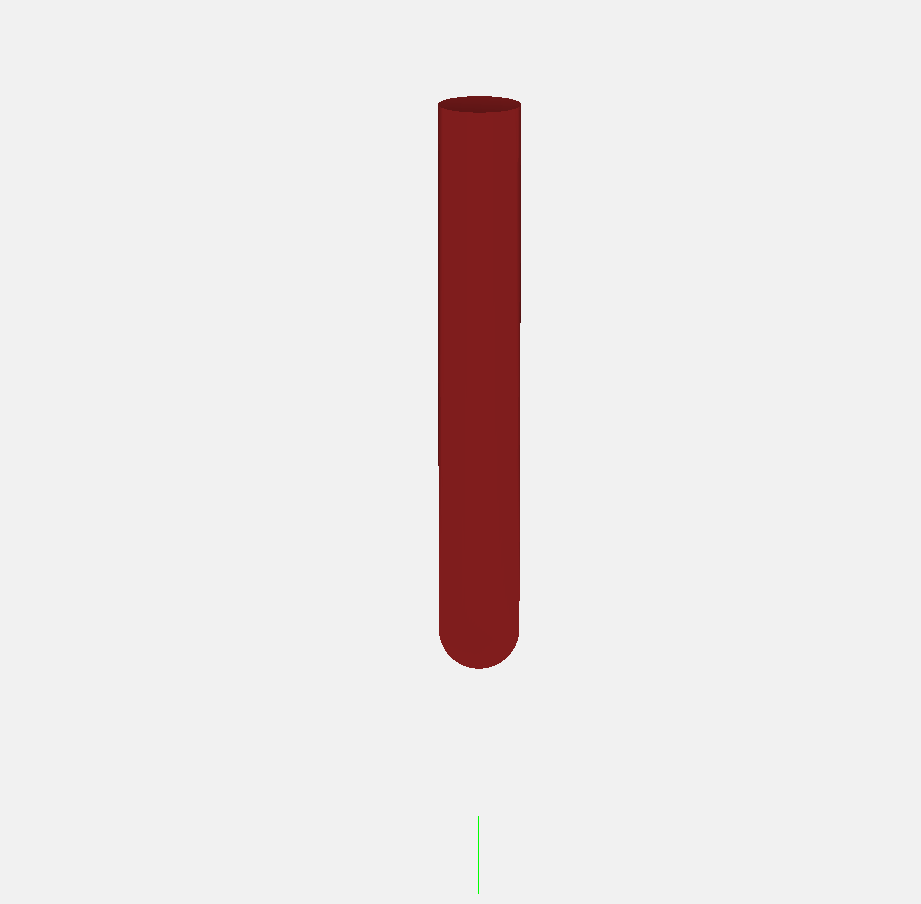
\includegraphics[width=\linewidth/3]{images/tool_ball_202.png}%
           
\includegraphics[width=\linewidth/3]{images/tool_V_301.png}%

\begin{itemize}
\item Square (\#201 and 102) --- able to cut a flat bottom, perpendicular side and
                                 right angle, their simple and easily understood 
                                 geometry makes them a standard choice 
\item Ballnose (\#202 and 101) --- rounded, they are the standard choice for concave
                                   and organic shapes
\item V tooling (\#301, 302 and 390) --- pointed at the tip, they are available in a
                                         variety of angles and diameters and may be
                                         used for decorative V carving, or for
                                         chamfering or cutting specific angles
\end{itemize}
\end{samepage}

Most tools are easily implemented with concise \textsc{3d} descriptions which may be connected with a simple \texttt{hull} operation. Note that extending the normal case to a pair of such operations, one for the shaft, the other for the cutting shape will markedly simplify the code, and will make it possible to colour-code the shaft which may afford indication of instances of it rubbing against the stock.

The \DescribeRoutine{endmill square} is a simple cylinder:

\lstset{firstnumber=\thegcpy}
\begin{writecode}{a}{gcodepreview.py}{python}
    def endmill_square(self, es_diameter, es_flute_length):
        return cylinder(r1=(es_diameter / 2), r2=(es_diameter / 2), h=es_flute_length, center = False)

\end{writecode}
\addtocounter{gcpy}{3}

The \DescribeRoutine{ballnose} is modeled as a hemisphere joined with a cylinder:

\lstset{firstnumber=\thegcpy}
\begin{writecode}{a}{gcodepreview.py}{python}
    def ballnose(self, es_diameter, es_flute_length):
        b = sphere(r=(es_diameter / 2))
        s = cylinder(r1=(es_diameter / 2), r2=(es_diameter / 2), h=es_flute_length, center=False)
        p = union(b, s)
        return p.translate([0, 0, (es_diameter / 2)])

\end{writecode}
\addtocounter{gcpy}{6}

The \DescribeRoutine{endmill v} is modeled as a cylinder with a zero width base and a second cylinder for the shaft (note that Python's \verb|math| defaults to radians, hence the need to convert from degrees):

\lstset{firstnumber=\thegcpy}
\begin{writecode}{a}{gcodepreview.py}{python}
    def endmill_v(self, es_v_angle, es_diameter):
        es_v_angle = math.radians(es_v_angle)
        v = cylinder(r1=0, r2=(es_diameter / 2), h=((es_diameter / 2) / math.tan((es_v_angle / 2))), center=False)
        s = cylinder(r1=(es_diameter / 2), r2=(es_diameter / 2), h=((es_diameter * 8) ), center=False)
        sh = s.translate([0, 0, ((es_diameter / 2) / math.tan((es_v_angle / 2)))])
        return union(v, sh)

\end{writecode}
\addtocounter{gcpy}{7}

The \DescribeRoutine{bowl tool} is modeled as a series of cylinders stacked on top of each other and \verb|hull()|ed together:

\lstset{firstnumber=\thegcpy}
\begin{writecode}{a}{gcodepreview.py}{python}
    def bowl_tool(self, radius, diameter, height):
        bts = cylinder(height - radius, diameter / 2, diameter / 2, center=False)
        bts = bts.translate([0, 0, radius])
        bts = bts.union(cylinder(height, diameter / 2 - radius, diameter / 2 - radius, center=False))
        for i in range(90):
#            print(math.sin(math.radians(i)))
            slice = cylinder((radius / 90), ((diameter / 2 - radius) + radius * math.sin(math.radians(i))), ((diameter / 2 - radius) + radius * math.sin(math.radians(i + 1))), center=False)
            bts = hull(bts, slice.translate([0, 0, (radius - radius * math.cos(math.radians(i)))]))
        return bts

\end{writecode}
\addtocounter{gcpy}{10}

The \DescribeRoutine{tapered ball} nose tool is modeled as a sphere at the tip and a pair of cylinders, where one (a cone) describes the taper, while the other represents the shaft.

One vendor which provides such tooling is Precise Bits: \url{https://www.precisebits.com/products/carbidebits/taperedcarve250b2f.asp&filter=7}, but unfortunately, their tool numbering is ambiguous, the version of each major number (204 and 304) for their $1/4^{\prime\prime}$ shank tooling which is sufficiently popular to also be offered in a ZRN coating will be used. Similarly, the \#501 and \#502 PCB engravers from Carbide \textsc{3d} will also be supported.

\lstset{firstnumber=\thegcpy}
\begin{writecode}{a}{gcodepreview.py}{python}
    def tapered_ball(self, es_tip, es_diameter, es_flute_length, es_angle):
        b = sphere(r=(es_tip / 2))
        s = cylinder(r1=(es_tip / 2), r2=(es_diameter / 2), h=es_flute_length, center=False)
        p = union(b, s)
        return p.translate([0, 0, (es_tip / 2)])

\end{writecode}
\addtocounter{gcpy}{6}

The \DescribeRoutine{flat V} tool is modeled as a cylinder with two different diameters, forming a truncated cone.

\lstset{firstnumber=\thegcpy}
\begin{writecode}{a}{gcodepreview.py}{python}
    def flat_V(self, es_tip, es_diameter, es_flute_length, es_angle):
        c = cylinder(r1=(es_tip / 2), r2=(es_diameter / 2), h=es_flute_length, center=False)
        return c

\end{writecode}
\addtocounter{gcpy}{4}

%\begin{verbatim}
%//!OpenSCAD
%
%module bowl_tool(radius, diameter, height) {
%  union(){
%    // chain hull
%    for (i = [1 : abs(1) : 90 - 1]) {
%      hull() {
%      translate([0, 0, (radius - radius * cos(i))]){
%        cylinder(r1=((diameter / 2 - radius) + radius * sin(i)), r2=((diameter / 2 - radius) + radius * sin((i + 1))), h=(radius / 90), center=false);
%      }
%      translate([0, 0, (radius - radius * cos((i + 1)))]){
%        cylinder(r1=((diameter / 2 - radius) + radius * sin((i + 1))), r2=((diameter / 2 - radius) + radius * sin(((i + 1) + 1))), h=(radius / 90), center=false);
%      }
%      }  // end hull (in loop)
%     } // end loop
%
%    translate([0, 0, radius]){
%      cylinder(r1=(diameter / 2), r2=(diameter / 2), h=(height - radius), center=false);
%    }
%    cylinder(r1=(diameter / 2 - radius), r2=(diameter / 2 - radius), h=height, center=false);
%  }
%}
%
%bowl_tool(6.35, 19.05, 15.875);
%\end{verbatim}

\paragraph{Tooling for Undercutting Toolpaths}

There are several notable candidates for under\-cutting tooling. \label{para:undercuttooling} 

\begin{itemize}
\item Keyhole tools --- intended to cut slots for retaining hardware used for picture
                        hanging, they may be used to create slots for other purposes
                        Note that it will be necessary to model these thrice, once for
                        the actual keyhole cutting, second for the fluted portion of
                        the shaft, and then the shaft should be modeled for collision
                        \url{https://assetssc.leevalley.com/en-gb/shop/tools/power-tool-accessories/router-bits/30113-keyhole-router-bits} 
\item Dovetail cutters --- used for the joinery of the same name, they cut a large
                           area at the bottom which slants up to a narrower region
                           at a defined angle
\item Lollipop cutters --- normally used for \textsc{3d} work, as their name suggests
                           they are essentially a (cutting) ball on a narrow stick
                           (the tool shaft), they are mentioned here only for
                           compleatness' sake and are not (at this time) implemented
\item Threadmill --- used for cutting threads, normally a single form geometry is
                     used on a CNC.
\end{itemize}

\subparagraph{Keyhole tools}

Keyhole toolpaths (see: subsection~\ref{subsec:keyholetoolpaths} are intended for use with tooling which projects beyond the the narrower shaft and so will cut usefully underneath the visible surface. Also described as ``undercut'' tooling, but see below.

\includeimage{keyhole_router_bits.pdf}%

The \DescribeRoutine{keyhole} is modeled in two parts, first the cutting base:

\lstset{firstnumber=\thegcpy}
\begin{writecode}{a}{gcodepreview.py}{python}
    def keyhole(self, es_diameter, es_flute_length):
        return cylinder(r1=(es_diameter / 2), r2=(es_diameter / 2), h=es_flute_length, center=False)

\end{writecode}
\addtocounter{gcpy}{3}

\noindent and a second call for an additional cylinder for the shaft will be necessary:

\lstset{firstnumber=\thegcpy}
\begin{writecode}{a}{gcodepreview.py}{python}
    def keyhole_shaft(self, es_diameter, es_flute_length):
        return cylinder(r1=(es_diameter / 2), r2=(es_diameter / 2), h=es_flute_length, center=False)

\end{writecode}
\addtocounter{gcpy}{3}

%TODO rework for shaft

\subparagraph{Thread mills}

\label{subpara:threadmills}The implementation of arcs cutting along the Z-axis raises the 
possibility of cutting threads using a \DescribeRoutine{threadmill}. 
See: \url{https://community.carbide3d.com/t/thread-milling-in-metal-on-the-shapeoko-3/5332}.

\lstset{firstnumber=\thegcpy}
\begin{writecode}{a}{gcodepreview.py}{python}
    def threadmill(self, minor_diameter, major_diameter, cut_height):
        btm = cylinder(r1=(minor_diameter / 2), r2=(major_diameter / 2), h=cut_height, center = False)
        top = cylinder(r1=(major_diameter / 2), r2=(minor_diameter / 2), h=cut_height, center = False)
        top = top.translate([0, 0, cut_height/2])
        tm = btm.union(top)
        return tm

    def threadmill_shaft(self, diameter, cut_height, height):
        shaft = cylinder(r1=(diameter / 2), r2=(diameter / 2), h=height, center = False)
        shaft = shaft.translate([0, 0, cut_height/2])
        return shaft

\end{writecode}
\addtocounter{gcpy}{12}

\subparagraph{Dovetails}

\label{subpara:dovetails}The \DescribeRoutine{dovetail} is modeled as a cylinder with the differing bottom and top diameters determining the angle (though \verb|dt_angle| is still required as a parameter)

\lstset{firstnumber=\thegcpy}
\begin{writecode}{a}{gcodepreview.py}{python}
    def dovetail(self, dt_bottomdiameter, dt_topdiameter, dt_height, dt_angle):
        return cylinder(r1=(dt_bottomdiameter / 2), r2=(dt_topdiameter / 2), h= dt_height, center=False)

\end{writecode}
\addtocounter{gcpy}{3}

\paragraph{Concave toolshapes}
\label{para:concavetoolshapes} 
While normal tooling may be represented with a one (or more) \texttt{hull} operation(s) betwixt two \textsc{3d} toolshapes (or six in the instance of keyhole tools), concave tooling such as roundover/radius tooling require multiple sections or even slices of the tool shape to be modeled separately which are then \texttt{hull}ed together. Something of this can be seen in the manual work-around for previewing them: \url{https://community.carbide3d.com/t/using-unsupported-tooling-in-carbide-create-roundover-cove-radius-bits/43723}.

Because it is necessary to divide the tooling into vertical slices and call the hull operation for each slice the tool definitions have to be called separately in the \verb|cut...| modules, or integrated at the lowest level.

%TODO move Roundover cuts into cutshape

\paragraph{Roundover tooling}

\label{para:roundover} It is not possible to represent all tools using tool changes as coded above which require using a \texttt{hull} operation between \textsc{3d} representations of the tools at the beginning and end points. Tooling which cannot be so represented will be implemented separately below, see paragraph~\ref{para:concavetoolshapes}.

\lstset{firstnumber=\thegcpscad}
\begin{writecode}{a}{gcodepreview.scad}{scad}
module cutroundover(bx, by, bz, ex, ey, ez, radiustn) {
    if (radiustn == 56125) {
        cutroundovertool(bx, by, bz, ex, ey, ez, 0.508/2, 1.531);
    } else if (radiustn == 56142) {
        cutroundovertool(bx, by, bz, ex, ey, ez, 0.508/2, 2.921);
//    } else if (radiustn == 312) {
//        cutroundovertool(bx, by, bz, ex, ey, ez, 1.524/2, 3.175);
    } else if (radiustn == 1570) {
        cutroundovertool(bx, by, bz, ex, ey, ez, 0.507/2, 4.509);
    }
}

\end{writecode}
\addtocounter{gcpscad}{12}

\noindent which then calls the actual \texttt{cutroundovertool} module passing in the tip radius and the radius of the rounding. Note that this module sets its quality relative to the value of \verb|$fn|.

\subsubsection{toolchange}

Then apply the appropriate commands for a \label{subsubsec:toolchange} \DescribeRoutine{toolchange}. Note that it is expected that this code will be updated as needed when new tooling is introduced as additional modules which require specific tooling are added. 

Note that the comments written out in G-code correspond to those used by the G-code previewing tool CutViewer (which is unfortunately, no longer readily available). Similarly, the G-code previewing functionality in this library expects that such comments will be in place so as to model the stock.

A further concern is that early versions often passed the tool into a module using a parameter. That ceased to be necessary in the 2024.09.03 version of PythonSCAD, and all modules should read the tool \# from \verb|currenttoolnumber()|. %Note that this variable has changed names from the original \verb|currenttool| which is now used to store the current tool \emph{shape} (or \textsc{3d} model).

%It is possible that rather than hard-coding the tool definitions, a future update will instead read them in from an external file --- the \texttt{.csv} format used for tool libraries in Carbide Create seems a likely candidate and worth exploring.

Note that there are many varieties of tooling and not all will be directly supported, and that at need, additional tool shape support may be added under \verb|misc|.
 
\paragraph{Selecting Tools}
 
The original implementation created the model for the tool at the current position, and a duplicate at the end position, wrapping the twain for each end of a given movement in a \verb|hull()| command. This approach will not work within Python, so it will be necessary to instead assign and select the tool as part of the cutting command indirectly by first storing it in the variable \DescribeVariable{currenttoolshape} (if the toolshape will work with the \verb|hull| command) which may be done in this module, or it will be necessary to check for the specific toolnumber in the \verb|cutline| module and handle the tooling in a separate module as is currently done for roundover tooling.

\lstset{firstnumber=\thegcpy}
\begin{writecode}{a}{gcodepreview.py}{python}
    def currenttool(self):
#        global currenttoolshape
        return self.currenttoolshape

\end{writecode}
\addtocounter{gcpy}{4}

Note that it will also be necessary to write out a tool description compatible with the program CutViewer as a G-code comment so that it may be used as a \textsc{3d} previewer for the G-code for tool changes in G-code. Several forms are available:

\paragraph{Square and ball nose (including tapered ball nose)}

\begin{verbatim}
TOOL/MILL, Diameter, Corner radius, Height, Taper Angle
\end{verbatim}

\paragraph{Roundover (corner rounding)}

\begin{verbatim}
TOOL/CRMILL, Diameter1, Diameter2, Radius, Height, Length
\end{verbatim}

\paragraph{Dovetails}

Unfortunately, tools which support undercuts such as dovetails are not supported by CutViewer (CAMotics will work for such tooling, at least dovetails which may be defined as "stub" endmills with a bottom diameter greater than upper diameter).

\paragraph{toolchange routine}

The Python definition for toolchange requires the tool number (used to write out the G-code comment description for CutViewer and also expects the speed for the current tool since this is passed into the G-code tool change command as part of the spindle on command.

\lstset{firstnumber=\thegcpy}
\begin{writecode}{a}{gcodepreview.py}{python}
    def toolchange(self, tool_number, speed = 10000):
#        global currenttoolshape
        self.currenttoolshape = self.endmill_square(0.001, 0.001)    
            
        self.settool(tool_number)
        if (self.generategcode == True):
            self.writegc("(Toolpath)")
            self.writegc("M05")
        if (tool_number == 201):
            self.writegc("(TOOL/MILL, 6.35, 0.00, 0.00, 0.00)")
            self.currenttoolshape = self.endmill_square(6.35, 19.05)
        elif (tool_number == 102):
            self.writegc("(TOOL/MILL, 3.175, 0.00, 0.00, 0.00)")
            self.currenttoolshape = self.endmill_square(3.175, 12.7)
        elif (tool_number == 112):
            self.writegc("(TOOL/MILL, 1.5875, 0.00, 0.00, 0.00)")
            self.currenttoolshape = self.endmill_square(1.5875, 6.35)
        elif (tool_number == 122):
            self.writegc("(TOOL/MILL, 0.79375, 0.00, 0.00, 0.00)")
            self.currenttoolshape = self.endmill_square(0.79375, 1.5875)
        elif (tool_number == 202):
            self.writegc("(TOOL/MILL, 6.35, 3.175, 0.00, 0.00)")
            self.currenttoolshape = self.ballnose(6.35, 19.05)
        elif (tool_number == 101):
            self.writegc("(TOOL/MILL, 3.175, 1.5875, 0.00, 0.00)")
            self.currenttoolshape = self.ballnose(3.175, 12.7)
        elif (tool_number == 111):
            self.writegc("(TOOL/MILL, 1.5875, 0.79375, 0.00, 0.00)")
            self.currenttoolshape = self.ballnose(1.5875, 6.35)
        elif (tool_number == 121):
            self.writegc("(TOOL/MILL, 3.175, 0.79375, 0.00, 0.00)")
            self.currenttoolshape = self.ballnose(0.79375, 1.5875)
        elif (tool_number == 327):
            self.writegc("(TOOL/MILL, 0.03, 0.00, 13.4874, 30.00)")
            self.currenttoolshape = self.endmill_v(60, 26.9748)
        elif (tool_number == 301):
            self.writegc("(TOOL/MILL, 0.03, 0.00, 6.35, 45.00)")
            self.currenttoolshape = self.endmill_v(90, 12.7)
        elif (tool_number == 302):
            self.writegc("(TOOL/MILL, 0.03, 0.00, 10.998, 30.00)")
            self.currenttoolshape = self.endmill_v(60, 12.7)
        elif (tool_number == 390):
            self.writegc("(TOOL/MILL, 0.03, 0.00, 1.5875, 45.00)")
            self.currenttoolshape = self.endmill_v(90, 3.175)
        elif (tool_number == 374):
            self.writegc("(TOOL/MILL, 9.53, 0.00, 3.17, 0.00)")
        elif (tool_number == 375):
            self.writegc("(TOOL/MILL, 9.53, 0.00, 3.17, 0.00)")
        elif (tool_number == 376):
            self.writegc("(TOOL/MILL, 12.7, 0.00, 4.77, 0.00)")
        elif (tool_number == 378):
            self.writegc("(TOOL/MILL, 12.7, 0.00, 4.77, 0.00)")
        elif (tool_number == 814):
            self.writegc("(TOOL/MILL, 12.7, 6.367, 12.7, 0.00)")
        #    dt_bottomdiameter, dt_topdiameter, dt_height, dt_angle)
        #    https://www.leevalley.com/en-us/shop/tools/power-tool-accessories/router-bits/30172-dovetail-bits?item=18J1607
            self.currenttoolshape = self.dovetail(12.7, 6.367, 12.7, 14)
    #    45828
        elif (tool_number == 808079):
            self.writegc("(TOOL/MILL, 12.7, 6.816, 20.95, 0.00)")
        #    http://www.amanatool.com/45828-carbide-tipped-dovetail-8-deg-x-1-2-dia-x-825-x-1-4-inch-shank.html
            self.currenttoolshape = self.dovetail(12.7, 6.816, 20.95, 8)
        elif (tool_number == 56125):#0.508/2, 1.531
            self.writegc("(TOOL/CRMILL, 0.508, 6.35, 3.175, 7.9375, 3.175)")
        elif (tool_number == 56142):#0.508/2, 2.921
            self.writegc("(TOOL/CRMILL, 0.508, 3.571875, 1.5875, 5.55625, 1.5875)")
#        elif (tool_number == 312):#1.524/2, 3.175
#            self.writegc("(TOOL/CRMILL, Diameter1, Diameter2, Radius, Height, Length)")
        elif (tool_number == 1570):#0.507/2, 4.509
            self.writegc("(TOOL/CRMILL, 0.17018, 9.525, 4.7625, 12.7, 4.7625)")
#https://www.amanatool.com/45982-carbide-tipped-bowl-tray-1-4-radius-x-3-4-dia-x-5-8-x-1-4-inch-shank.html 
        elif (tool_number == 45982):#0.507/2, 4.509
            self.writegc("(TOOL/MILL, 15.875, 6.35, 19.05, 0.00)")
            self.currenttoolshape = self.bowl_tool(6.35, 19.05, 15.875)
        elif (tool_number == 204):#
            self.writegc("()")
            self.currenttoolshape = self.tapered_ball(1.5875, 6.35, 38.1, 3.6)
        elif (tool_number == 304):#
            self.writegc("()")
            self.currenttoolshape = self.tapered_ball(3.175, 6.35, 38.1, 2.4)
        elif (tool_number == 501):#
            self.writegc("()")
            self.currenttoolshape = self.tapered_ball(0.127, 3.175, 2.688, 60)
        elif (tool_number == 502):#
            self.writegc("()")
            self.currenttoolshape = self.tapered_ball(0.127, 3.175, 4.25, 40)
        elif (tool_number == 13921):#
            self.writegc("()")
            self.currenttoolshape = self.flat_V(6.35, 31.75, 12.7, 45)
\end{writecode}
\addtocounter{gcpy}{89}

\noindent With the tools delineated, the module is closed out and the toolchange information written into the G-code as well as the command to start the spindle at the specified speed.
 
\lstset{firstnumber=\thegcpy}
\begin{writecode}{a}{gcodepreview.py}{python}
        self.writegc("M6T", str(tool_number))
        self.writegc("M03S", str(speed))

\end{writecode}
\addtocounter{gcpy}{3}

%Note that the \verb|if...else| constructs will need to be extended into the command \verb|cutline| for those toolshapes (keyhole, roundover, \&c.) which will not work with a straight-forward \verb|hull...| implementation.

As per usual, the OpenSCAD command is simply a dispatcher:

\lstset{firstnumber=\thegcpscad}
\begin{writecode}{a}{gcodepreview.scad}{scad}
module toolchange(tool_number, speed){
    gcp.toolchange(tool_number, speed);
}

\end{writecode}
\addtocounter{gcpscad}{4}

\noindent For example:

\begin{verbatim}
toolchange(small_square_tool_num, speed);
\end{verbatim}

\noindent (the assumption is that all speed rates in a file will be the same, so as to account for the most frequent use case of a trim router with speed controlled by a dial setting and feed rates/ratios being calculated to provide the correct chipload at that setting.)

\subsubsection{tooldiameter}

It will also be necessary to be able to provide the diameter of the current tool. Arguably, this would be much easier using an object-oriented programming style/dot notation.

One aspect of tool parameters which will need to be supported is shapes which create different profiles based on how deeply the tool is cutting into the surface of the material at a given point. To accommodate this, it will be necessary to either track the thickness of uncut material at any given point, or, to specify the depth of cut as a parameter.

% which is what the initial version will implement.

The public-facing OpenSCAD code, \DescribeRoutine{tool diameter} simply calls the matching OpenSCAD module which wraps the Python code:
 
\lstset{firstnumber=\thegcpscad}
\begin{writecode}{a}{gcodepreview.scad}{scad}
function tool_diameter(td_tool, td_depth) = otool_diameter(td_tool, td_depth);

\end{writecode}
\addtocounter{gcpscad}{2}

\noindent the Python code, \DescribeRoutine{tool diameter} returns 
appropriate values based on the specified tool number and depth:
 
\lstset{firstnumber=\thegcpy}
\begin{writecode}{a}{gcodepreview.py}{python}
    def tool_diameter(self, ptd_tool, ptd_depth):
# Square 122, 112, 102, 201
        if ptd_tool == 122:
            return 0.79375
        if ptd_tool == 112:
            return 1.5875
        if ptd_tool == 102:
            return 3.175
        if ptd_tool == 201:
            return 6.35
# Ball 121, 111, 101, 202
        if ptd_tool == 122:
            if ptd_depth > 0.396875:
                return 0.79375
            else:
                return ptd_tool
        if ptd_tool == 112:
            if ptd_depth > 0.79375:
                return 1.5875
            else:
                return ptd_tool
        if ptd_tool == 101:
            if ptd_depth > 1.5875:
                return 3.175
            else:
                return ptd_tool
        if ptd_tool == 202:
            if ptd_depth > 3.175:
                return 6.35
            else:
                return ptd_tool
# V 301, 302, 390
        if ptd_tool == 301:
            return ptd_tool
        if ptd_tool == 302:
            return ptd_tool
        if ptd_tool == 390:
            return ptd_tool
# Keyhole
        if ptd_tool == 374:
            if ptd_depth < 3.175:
                return 9.525
            else:
                return 6.35
        if ptd_tool == 375:
            if ptd_depth < 3.175:
                return 9.525
            else:
                return 8
        if ptd_tool == 376:
            if ptd_depth < 4.7625:
                return 12.7
            else:
                return 6.35
        if ptd_tool == 378:
            if ptd_depth < 4.7625:
                return 12.7
            else:
                return 8
# Dovetail
        if ptd_tool == 814:
            if ptd_depth > 12.7:
                return 6.35
            else:
                return ptd_tool
        if ptd_tool == 808079:
            if ptd_depth > 20.95:
                return 6.816
            else:
                return ptd_tool
# Bowl Bit
#https://www.amanatool.com/45982-carbide-tipped-bowl-tray-1-4-radius-x-3-4-dia-x-5-8-x-1-4-inch-shank.html 
        if ptd_tool == 45982:
            if ptd_depth > 6.35:
                return 15.875
            else:
                return ptd_tool
# Tapered Ball Nose
        if ptd_tool == 204:
            if ptd_depth > 6.35:
                return ptd_tool
        if ptd_tool == 304:
            if ptd_depth > 6.35:
                return ptd_tool
            else:
                return ptd_tool

\end{writecode}
\addtocounter{gcpy}{87}

Since it is often necessary to utilise the radius of the tool, an additional command, \DescribeRoutine{tool radius} to return this value is worthwhile:
 
\lstset{firstnumber=\thegcpy}
\begin{writecode}{a}{gcodepreview.py}{python}
    def tool_radius(self, ptd_tool, ptd_depth):
        tr = self.tool_diameter(ptd_tool, ptd_depth)/2
        return tr

\end{writecode}
\addtocounter{gcpy}{4}
 
\noindent (Note that where values are not fully calculated values currently the passed in tool number (\verb|ptd tool|)is returned which will need to be replaced with code which calculates the appropriate values.)

\subsubsection{Feeds and Speeds}

There are several possibilities for handling feeds and speeds. Currently, base values for \DescribeVariable{feed}, \DescribeVariable{plunge}, and \DescribeVariable{speed} are used, which may then be adjusted using various \verb|<tooldescriptor>_ratio| values, as an acknowledgement of the likelihood of a trim router being used as a spindle, the assumption is that the \texttt{speed} will remain unchanged.

%One notable possibility for the future would be to load it from the .csv files used for User tool libraries in Carbide Create. Ideally, any use of such values in modules would be such that some other scheme could replace that usage with minimal editing and updating.

The tools which need to be calculated thus are those in addition to the \verb|large_square| tool:

\begin{itemize}
\item \verb|small_square_ratio|
\item \verb|small_ball_ratio|
\item \verb|large_ball_ratio|
\item \verb|small_V_ratio|
\item \verb|large_V_ratio|
\item \verb|KH_ratio|
\item \verb|DT_ratio|
\end{itemize}

\subsection{Movement and Cutting}

With all the scaffolding in place, it is possible to model the tool and \verb|hull()| between copies of the \textsc{3d} model of the tool, or a cross-section of it for both \DescribeRoutine{cut...} and \DescribeRoutine{rapid...} operations.

%\DescribeRoutine{otm}, (colors the tool model so as to differentiate cut areas) and cutting: \DescribeSubroutine{cut}{ocut}, as well as Rapid movements to position the tool to begin a cut: \DescribeSubroutine{rapid}{orapid}, \DescribeRoutine{rapid}, and \DescribeRoutine{rapidbx} which will also need to write out files which represent the desired machine motions.

Note that the variables \verb|self.rapids| and \verb|self.toolpaths| are used to hold the accumulated (\verb|unioned|) \textsc{3d} models of the rapid motions and cuts so that they may be \verb|difference|d from the stock when the value \verb|generatepaths| is set to \verb|True|.

In order to manage the various options when cutting it will be necessary to have a command where the actual cut is made, passing in the shape used for the cut as a parameter. Since the \textsc{3d} aspect of \verb|rapid| and \verb|cut| operations are fundamentally the same, the command \DescribeRoutine{rcs} which returns the \verb|hull| of the begin (the current machine position as accessed by the \verb|x/y/zpos()| commands and end positioning (provided as arguments \verb|ex|, \verb|ey|, and \verb|ez|) of the tool shape/cross-section will be defined for the common aspects:

\lstset{firstnumber=\thegcpy}
\begin{writecode}{a}{gcodepreview.py}{python}
    def rcs(self, ex, ey, ez, shape):
        start = shape
        end = shape
        toolpath = hull(start.translate([self.xpos(), self.ypos(), self.zpos()]), 
                        end.translate([ex, ey, ez]))
        return toolpath

\end{writecode}
\addtocounter{gcpy}{7}

Diagramming this is quite straight-forward --- there is simply a movement made from the current position to the end. If we start at the origin, \verb|X0|, \verb|Y0|, \verb|Z0|, then it is simply a straight-line movement (rapid)/cut (possibly a partial cut in the instance of a keyhole or roundover tool), and no variables change value.

The code for diagramming this is quite straight-forward. A BlockSCAD implementation is available at: \url{https://www.blockscad3d.com/community/projects/1894400}, and the OpenSCAD version is only a little more complex (adding code to ensure positioning):

\includeimage{gcp_statemachine_0_0_0_50_25_-10.png}%

%TODO ADD BELOW !!!!!!!!!!!!!!!!!!!!!!!!!!!!!!!!!!!!!!!!!!!!!!!!!!!!!!!!!!!!!!!!!!!!!!!!!!!!!!
%
%\begin{verbatim}
%
%\subsection{Shapes and tool movement}
% 
%The majority of commands will be more general, focusing on tooling which is generally supported by this library, moving in lines and arcs so as to describe shapes which lend themselves to representation with those tool and which match up with both toolpaths and supported geometry in Carbide Create, and the usage requirements of the typical user.
%
%\subsubsection{Generalized commands and cuts}
%
%The first consideration is a naming convention which will allow a generalized set of associated commands to be defined. The initial version will only create OpenSCAD commands for 3D modeling and write out matching DXF files. At a later time this will be extended with G-code support.
% 
%\paragraph{begincutdxf}
% 
%The first command, \DescribeRoutine{begincutdxf} will need to allow the machine to rapid to the beginning point of the cut and then rapid down to the surface of the stock, and then plunge down to the depth of the cut. The implementation will need to allow for a hook where the Depth per Pass is applied to the plunge operation so that multiple passes are made.
%
%The first module will ensure that the tool is safely up above the stock and will rapid to the position specified at the retract height (moving to that position as an initial step, then will \texttt{cutwithfeed} to the specified position at the specified feed rate. Despite \texttt{dxf} being included in the filename no change is made to the dxf file at this time, this simply indicates that this file is preparatory to the use of \DescribeRoutine{continuecutdxf}.
%
%\lstset{firstnumber=\thegcpscad}
%\begin{writecode}{a}{gcodepreview.scad}{scad}
%module begincutdxf(rh, ex, ey, ez, fr) {
%  rapid(getxpos(), getypos(), rh);
%  cutwithfeed(ex, ey, ez, fr);
%}
%
%\end{writecode}
%\addtocounter{gcpscad}{5}
% 
%\lstset{firstnumber=\thegcpscad}
%\begin{writecode}{a}{gcodepreview.scad}{scad}
%module continuecutdxf(ex, ey, ez, fr) {
%  cutwithfeed(ex, ey, ez, fr);
%}
%
%\end{writecode}
%\addtocounter{gcpscad}{4}
%\end{verbatim}

\noindent Note that this routine does \emph{not} alter the machine position variables since it may be called multiple times for a given toolpath. This command will then be called in the definitions for \verb|rapid| and \verb|cutshape| which only differ in which variable the \textsc{3d} model is \verb|union|ed with:

There are three different movements in G-code which will need to be handled. Rapid commands will be used for \textsc{g0} movements and will not appear in \textsc{dxf}s but will appear in G-code files, while straight line cut (\textsc{g1}) and arc (\textsc{g2/g3}) commands may appear in both G-code and \textsc{dxf} files, depending on the specific command invoked. 

\lstset{firstnumber=\thegcpy}
\begin{writecode}{a}{gcodepreview.py}{python}
    def rapid(self, ex, ey, ez):
        cts = self.currenttoolshape
        toolpath = self.rcs(ex, ey, ez, cts)
        self.setxpos(ex)
        self.setypos(ey)
        self.setzpos(ez)
        if self.generatepaths == True:
            self.rapids = self.rapids.union(toolpath)
#            return cylinder(0.01, 0, 0.01, center = False, fn = 3)
            return cube([0.001, 0.001, 0.001])
        else:
            return toolpath

    def cutshape(self, ex, ey, ez):
        cts = self.currenttoolshape
        toolpath = self.rcs(ex, ey, ez, cts)
        if self.generatepaths == True:
            self.toolpaths = self.toolpaths.union(toolpath)
            return cube([0.001, 0.001, 0.001])
        else:
            return toolpath

\end{writecode}
\addtocounter{gcpy}{22}

Note that it is necessary to return a shape so that modules which use a \verb|<variable>.union| command will function as expected even when the \textsc{3d} model created is stored in a variable.

It is then possible to add specific \verb|rapid...| commands to match typical usages of G-code. The first command needs to be a move to/from the safe Z height. In G-code this would be:

\begin{verbatim}
(Move to safe Z to avoid workholding)
G53G0Z-5.000
\end{verbatim}

\noindent but in the \textsc{3d} model, since we do not know how tall the Z-axis is, we simply move to safe height and use that as a starting point:

\lstset{firstnumber=\thegcpy}
\begin{writecode}{a}{gcodepreview.py}{python}
    def movetosafeZ(self):
        rapid = self.rapid(self.xpos(), self.ypos(), self.retractheight)
#        if self.generatepaths == True:
#            rapid = self.rapid(self.xpos(), self.ypos(), self.retractheight)
#            self.rapids = self.rapids.union(rapid)
#        else:
#  if (generategcode == true) {
#  //    writecomment("PREPOSITION FOR RAPID PLUNGE");Z25.650
#  //G1Z24.663F381.0, "F", str(plunge)
        if self.generatepaths == False:
            return rapid
        else:
            return cube([0.001, 0.001, 0.001])

    def rapidXYZ(self, ex, ey, ez):
        rapid = self.rapid(ex, ey, ez)
        if self.generatepaths == False:
            return rapid

    def rapidXY(self, ex, ey):
        rapid = self.rapid(ex, ey, self.zpos())
#        if self.generatepaths == True:
#            self.rapids = self.rapids.union(rapid)
#        else:
        if self.generatepaths == False:
            return rapid

    def rapidXZ(self, ex, ez):
        rapid = self.rapid(ex, self.ypos(), ez)
        if self.generatepaths == False:
            return rapid

    def rapidYZ(self, ey, ez):
        rapid = self.rapid(self.xpos(), ey, ez)
        if self.generatepaths == False:
            return rapid

    def rapidX(self, ex):
        rapid = self.rapid(ex, self.ypos(), self.zpos())
        if self.generatepaths == False:
            return rapid

    def rapidY(self, ey):
        rapid = self.rapid(self.xpos(), ey, self.zpos())
        if self.generatepaths == False:
            return rapid

    def rapidZ(self, ez):
        rapid = self.rapid(self.xpos(), self.ypos(), ez)
#        if self.generatepaths == True:
#            self.rapids = self.rapids.union(rapid)
#        else:
        if self.generatepaths == False:
            return rapid

\end{writecode}
\addtocounter{gcpy}{55}

%Note that a hard-coded cylinder is used since the command will be used prior to a toolchange. In the future there may be a command for initializing the \DescribeVariable{toolpaths} so that later cut commands may add to it.

Note that rather than re-create the matching OpenSCAD commands as descriptors, due to the issue of redirection and return values and the possibility for errors it is more expedient to simply re-create the matching command (at least for the rapids):

\lstset{firstnumber=\thegcpscad}
\begin{writecode}{a}{gcodepreview.scad}{scad}
module movetosafeZ(){
    gcp.rapid(gcp.xpos(), gcp.ypos(), retractheight);
}

module rapid(ex, ey, ez) {
    gcp.rapid(ex, ey, ez);
}

module rapidXY(ex, ey) {
    gcp.rapid(ex, ey, gcp.zpos());
}

module rapidXZ(ex, ez) {
    gcp.rapid(ex, gcp.zpos(), ez);
}

module rapidZ(ez) {
    gcp.rapid(gcp.xpos(), gcp.ypos(), ez);
}

\end{writecode}
\addtocounter{gcpscad}{20}

\subsubsection{Lines}

The Python commands \DescribeRoutine{cut...} add the \verb|currenttool| to the \verb|toolpath| \verb|hull|ed together at the current position and the end position of the move. For \DescribeRoutine{cutline}, this is a straight-forward connection of the current (beginning) and ending coordinates:

\lstset{firstnumber=\thegcpy}
\begin{writecode}{a}{gcodepreview.py}{python}
    def cutline(self, ex, ey, ez):\
#below will need to be integrated into if/then structure not yet copied
#        cts = self.currenttoolshape
        if (self.currenttoolnumber() == 374):
#            self.writegc("(TOOL/MILL, 9.53, 0.00, 3.17, 0.00)")
            self.currenttoolshape = self.keyhole(9.53/2, 3.175)
            toolpath = self.cutshape(ex, ey, ez)
            self.currenttoolshape = self.keyhole_shaft(6.35/2, 12.7)
            toolpath = toolpath.union(self.cutshape(ex, ey, ez))
#        elif (self.currenttoolnumber() == 375):
#            self.writegc("(TOOL/MILL, 9.53, 0.00, 3.17, 0.00)")
#        elif (self.currenttoolnumber() == 376):
#            self.writegc("(TOOL/MILL, 12.7, 0.00, 4.77, 0.00)")
#        elif (self.currenttoolnumber() == 378):
#            self.writegc("(TOOL/MILL, 12.7, 0.00, 4.77, 0.00)")
#        elif (self.currenttoolnumber() == 56125):#0.508/2, 1.531
#            self.writegc("(TOOL/CRMILL, 0.508, 6.35, 3.175, 7.9375, 3.175)")
        elif (self.currenttoolnumber() == 56142):#0.508/2, 2.921
#            self.writegc("(TOOL/CRMILL, 0.508, 3.571875, 1.5875, 5.55625, 1.5875)")
            toolpath = self.cutroundovertool(self.xpos(), self.ypos(), self.zpos(), ex, ey, ez, 0.508/2, 1.531)
#        elif (self.currenttoolnumber() == 1570):#0.507/2, 4.509
#            self.writegc("(TOOL/CRMILL, 0.17018, 9.525, 4.7625, 12.7, 4.7625)")
        else:
            toolpath = self.cutshape(ex, ey, ez)
        self.setxpos(ex)
        self.setypos(ey)
        self.setzpos(ez)
#        if self.generatepaths == True:
#            self.toolpaths = union([self.toolpaths, toolpath])
#        else:
        if self.generatepaths == False:
            return toolpath
        else:
            return cube([0.001, 0.001, 0.001])

    def cutlinedxfgc(self, ex, ey, ez):
        self.dxfline(self.currenttoolnumber(), self.xpos(), self.ypos(), ex, ey)
        self.writegc("G01 X", str(ex), " Y", str(ey), " Z", str(ez))
#        if self.generatepaths == False:
        return self.cutline(ex, ey, ez)

    def cutvertexdxf(self, ex, ey, ez):
        self.addvertex(self.currenttoolnumber(), ex, ey)
#        self.writegc("G01 X", str(ex), " Y", str(ey), " Z", str(ez))
#        if self.generatepaths == False:
        return self.cutline(ex, ey, ez)

    def cutroundovertool(self, bx, by, bz, ex, ey, ez, tool_radius_tip, tool_radius_width, stepsizeroundover = 1):
#        n = 90 + fn*3
#        print("Tool dimensions", tool_radius_tip, tool_radius_width, "begin ", bx, by, bz, "end ", ex, ey, ez)
        step = 4 #360/n
        shaft = cylinder(step, tool_radius_tip, tool_radius_tip)
        toolpath = hull(shaft.translate([bx, by, bz]), shaft.translate([ex, ey, ez]))
        shaft = cylinder(tool_radius_width*2, tool_radius_tip+tool_radius_width, tool_radius_tip+tool_radius_width)
        toolpath = toolpath.union(hull(shaft.translate([bx, by, bz+tool_radius_width]), shaft.translate([ex, ey, ez+tool_radius_width])))
        for i in range(1, 90, stepsizeroundover):
            angle = i
            dx = tool_radius_width*math.cos(math.radians(angle))
            dxx = tool_radius_width*math.cos(math.radians(angle+1))
            dzz = tool_radius_width*math.sin(math.radians(angle))
            dz = tool_radius_width*math.sin(math.radians(angle+1))
            dh = abs(dzz-dz)+0.0001
            slice = cylinder(dh, tool_radius_tip+tool_radius_width-dx, tool_radius_tip+tool_radius_width-dxx)
            toolpath = toolpath.union(hull(slice.translate([bx, by, bz+dz]), slice.translate([ex, ey, ez+dz])))
        if self.generatepaths == True:
            self.toolpaths = self.toolpaths.union(toolpath)
        else:
            return toolpath

    def cutlineXYZwithfeed(self, ex, ey, ez, feed):
        return self.cutline(ex, ey, ez)

    def cutlineXYZ(self, ex, ey, ez):
        return self.cutline(ex, ey, ez)

    def cutlineXYwithfeed(self, ex, ey, feed):
        return self.cutline(ex, ey, self.zpos())

    def cutlineXY(self, ex, ey):
        return self.cutline(ex, ey, self.zpos())

    def cutlineXZwithfeed(self, ex, ez, feed):
        return self.cutline(ex, self.ypos(), ez)

    def cutlineXZ(self, ex, ez):
        return self.cutline(ex, self.ypos(), ez)

    def cutlineXwithfeed(self, ex, feed):
        return self.cutline(ex, self.ypos(), self.zpos())

    def cutlineX(self, ex):
        return self.cutline(ex, self.ypos(), self.zpos())

    def cutlineYZ(self, ey, ez):
        return self.cutline(self.xpos(), ey, ez)

    def cutlineYwithfeed(self, ey, feed):
        return self.cutline(self.xpos(), ey, self.zpos())

    def cutlineY(self, ey):
        return self.cutline(self.xpos(), ey, self.zpos())

    def cutlineZgcfeed(self, ez, feed):
        self.writegc("G01 Z", str(ez), "F", str(feed))
#        if self.generatepaths == False:
        return self.cutline(self.xpos(), self.ypos(), ez)

    def cutlineZwithfeed(self, ez, feed):
        return self.cutline(self.xpos(), self.ypos(), ez)

    def cutlineZ(self, ez):
        return self.cutline(self.xpos(), self.ypos(), ez)

\end{writecode}
\addtocounter{gcpy}{107}

%CODE TO RESTORE
%
%\begin{verbatim}
%#        global toolpath
%#        global toolpaths
%#        print("cutline tool #", self.currenttoolnumber())
%        if (self.currenttoolnumber() == 56142):
%#                print("cutline tool internal #", self.currenttoolnumber())
%            toolpath = self.cutroundovertool(self.xpos(), self.ypos(), self.zpos(), ex, ey, ez, 0.508/2, 1.531)
%        elif (self.currenttoolnumber() == 56125):
%            toolpath = self.cutroundovertool(self.xpos(), self.ypos(), self.zpos(), ex, ey, ez, 0.508/2, 2.921)
%#        elif (self.currenttoolnumber() == 312):
%#            toolpath = self.cutroundovertool(self.xpos(), self.ypos(), self.zpos(), ex, ey, ez, 1.524/2, 3.175)
%        elif (self.currenttoolnumber() == 1570):
%            toolpath = self.cutroundovertool(self.xpos(), self.ypos(), self.zpos(), ex, ey, ez, 0.507/2, 4.509)
%        elif (self.currenttoolnumber() == 374):
%#            self.writegc("(TOOL/MILL, 9.53, 0.00, 3.17, 0.00)")
%            shaft = cylinder(9.525, 6.35/2, 6.35/2)
%            shaftend = shaft
%            shaftbegin = shaft.translate([self.xpos(), self.ypos(), self.zpos()])
%            shaftpath = hull(shaftbegin, shaftend.translate([ex, ey, ez]))
%            start = cylinder(3.175, 9.525/2, 9.525/2)
%            end = start
%            start = start.translate([self.xpos(), self.ypos(), self.zpos()])
%            cutpath = hull(start, end.translate([ex, ey, ez]))
%            toolpath = union(shaftpath, cutpath)
%        elif (self.currenttoolnumber() == 375):
%#            self.writegc("(TOOL/MILL, 9.53, 0.00, 3.17, 0.00)")
%            shaft = cylinder(9.525, 8/2, 8/2)
%            shaftend = shaft
%            shaftbegin = shaft.translate([self.xpos(), self.ypos(), self.zpos()])
%            shaftpath = hull(shaftbegin, shaftend.translate([ex, ey, ez]))
%            start = cylinder(3.175, 9.525/2, 9.525/2)
%            end = start
%            start = start.translate([self.xpos(), self.ypos(), self.zpos()])
%            cutpath = hull(start, end.translate([ex, ey, ez]))
%            toolpath = union(shaftpath, cutpath)
%        elif (self.currenttoolnumber() == 376):
%#            self.writegc("(TOOL/MILL, 12.7, 0.00, 4.77, 0.00)")
%            shaft = cylinder(9.525, 6.35/2, 6.35/2)
%            shaftend = shaft
%            shaftbegin = shaft.translate([self.xpos(), self.ypos(), self.zpos()])
%            shaftpath = hull(shaftbegin, shaftend.translate([ex, ey, ez]))
%            start = cylinder(3.175, 12.7/2, 12.7/2)
%            end = start
%            start = start.translate([self.xpos(), self.ypos(), self.zpos()])
%            cutpath = hull(start, end.translate([ex, ey, ez]))
%            toolpath = union(shaftpath, cutpath)
%        elif (self.currenttoolnumber() == 378):
%#            self.writegc("(TOOL/MILL, 12.7, 0.00, 4.77, 0.00)")
%            shaft = cylinder(9.525, 8/2, 8/2)
%            shaftend = shaft
%            shaftbegin = shaft.translate([self.xpos(), self.ypos(), self.zpos()])
%            shaftpath = hull(shaftbegin, shaftend.translate([ex, ey, ez]))
%            start = cylinder(3.175, 12.7/2, 12.7/2)
%            end = start
%            start = start.translate([self.xpos(), self.ypos(), self.zpos()])
%            cutpath = hull(start, end.translate([ex, ey, ez]))
%            toolpath = union(shaftpath, cutpath)
%        elif (self.currenttoolnumber() == 648):
%            shaft = self.threadmill_shaft(2.4, 0.75, 18)
%            shaftend = shaft
%            shaftbegin = shaft.translate([self.xpos(), self.ypos(), self.zpos()])
%            shaftpath = hull(shaftbegin, shaftend.translate([ex, ey, ez]))
%            start = self.threadmill(2.4, 4.8, 0.75)
%            end = start
%            start = start.translate([self.xpos(), self.ypos(), self.zpos()])
%            cutpath = union(start, end.translate([ex, ey, ez]))
%            toolpath = union(shaftpath, cutpath)
%        else:
%%            start = self.currenttool()
%%            start = start.translate([self.xpos(), self.ypos(), self.zpos()])
%%            end = self.currenttool()
%%            toolpath = hull(start, end.translate([ex, ey, ez]))
%%        self.setxpos(ex)
%%        self.setypos(ey)
%%        self.setzpos(ez)
%%        if self.generatepaths == True:
%%            self.toolpaths = union([self.toolpaths, toolpath])
%%        else:
%%            return toolpath
%   
%    def cutlinedxfgcfeed(self, ex, ey, ez, feed):
%        self.dxfline(self.currenttoolnumber(), self.xpos(), self.ypos(), ex, ey)
%        self.writegc("G01 X", str(ex), " Y", str(ey), " Z", str(ez), " F", str(feed))
%#        if self.generatepaths == False:
%        return self.cutline(ex, ey, ez)
%
%
%\end{verbatim}

The matching OpenSCAD command is a descriptor:

\lstset{firstnumber=\thegcpscad}
\begin{writecode}{a}{gcodepreview.scad}{scad}
module cutline(ex, ey, ez){
    gcp.cutline(ex, ey, ez);
}

module cutlinedxfgc(ex, ey, ez){
    gcp.cutlinedxfgc(ex, ey, ez);
}

module cutlineZgcfeed(ez, feed){
    gcp.cutlineZgcfeed(ez, feed);
}

\end{writecode}
\addtocounter{gcpscad}{12}      

\subsubsection{Arcs for toolpaths and DXFs}
 
A further consideration here is that G-code and \textsc{dxf} support arcs in addition to the lines already implemented. Implementing arcs wants at least the following options for quadrant and direction:
 
\begin{itemize}
\item cutarcCW --- cut a partial arc described in a clock-wise direction
\item cutarcCC --- counter-clock-wise
\item cutarcNWCW --- cut the upper-left quadrant of a circle moving clockwise
\item cutarcNWCC --- upper-left quadrant counter-clockwise
\item cutarcNECW
\item cutarcNECC
\item cutarcSECW
\item cutarcSECC
\item cutarcNECW
\item cutarcNECC
\item cutcircleCC --- while it won't matter for generating a \textsc{dxf}, when G-code is implemented
                      direction of cut will be a consideration for that
\item cutcircleCW
\item cutcircleCCdxf
\item cutcircleCWdxf
\end{itemize}
 
It will be necessary to have two separate representations of arcs --- the G-code and \textsc{dxf} may be easily and directly supported with a single command, but representing the matching tool movement in OpenSCAD will require a series of short line movements which approximate the arc cutting in each direction and at changing Z-heights so as to allow for threading and similar operations. 
Note that there are the following representations/interfaces for representing an arc:

%At this time, the current version of Carbide Create only imports circles in \textsc{dxf} as curves, any other example is converted into polylines --- unfortunately, the implementation of this is not such as would allow directly matching that representation. A work-around to import a \textsc{dxf} as curves is to convert the arc into a reasonable number of line segments so as to approximate the arc.
 
\begin{itemize}
\item G-code --- \textsc{g2} (clockwise) and \textsc{g3} (counter-clockwise) arcs may be specified, 
      and since the endpoint is the positional requirement, it is most likely best to use the offset 
      to the center (\textsc{i} and \textsc{j}), rather than the radius parameter (\textsc{k}) 
      \texttt{G2/3 ...} 
\item \textsc{dxf} --- \texttt{dxfarc(xcenter, ycenter, radius, anglebegin, endangle, tn)}
\item approximation of arc using lines (OpenSCAD) in both clock-wise and counter-clock-wise directions
% --- note that this may also be used 
%      in \textsc{dxf} so as to sidestep the question of how many line segments there would be
%      for a given arc representation 
\end{itemize}
 
Cutting the quadrant arcs greatly simplifies the calculation and interface for the modules. A full set of 8 will be necessary, then circles will have a pair of modules (one for each cut direction) made for them.
 
%At this time, despite what the module names imply (\texttt{cutarcNWCWdxf}, \&c.), only cutting and \textsc{dxf} generation is supported. Adding support for G-code will be done at a later time. Since these modules will ultimately support G-code, the interface will assume the stored \texttt{xpos} and \texttt{ypos} as the origin. 

Parameters which will need to be passed in are:
 
\begin{itemize}
% \item \texttt{tn}
 \item \texttt{ex} --- note that the matching origins (\verb|bx|, \verb|by|, \verb|bz|) as well as 
                       the (current) toolnumber are accessed using the appropriate commands for machine position
 \item \texttt{ey}
 \item \texttt{ez} --- allowing a different Z position will make possible threading and
                       similar helical toolpaths
\item \texttt{xcenter} --- the center position will be specified as an absolute
      position which will require calculating the offset when it is used for 
      G-code's \texttt{IJ}, for which \texttt{xctr/yctr} are suggested 
\item \texttt{ycenter}
\item \texttt{radius} --- while this could be calculated, passing it in as a parameter
      is both convenient and (potentially) could be used as a check on the other
      parameters
\item \texttt{tpzreldim} --- the relative depth (or increase in height) of the
      current cutting motion
\end{itemize}

Since OpenSCAD does not have an arc movement command it is necessary to iterate through a loop: \DescribeRoutine{cutarcCW} (clockwise) or \DescribeRoutine{cutarcCC} (counterclockwise) to handle the drawing and processing of the \texttt{cutline()} toolpaths as short line segments which additionally affords a single point of control for adding additional features such as allowing the depth to  vary as one cuts along an arc (the line version is used rather than shape so as to capture the changing machine positions with each step through the loop). Note that the definition matches the \verb|DXF| definition of defining the center position with a matching radius, but it will be necessary to move the tool to the actual origin, and to calculate the end position when writing out a \verb|G2/G3| arc.

This brings to the fore the fact that at its heart, this program is simply graphing math in \textsc{3d} using tools (as presaged by the book series \emph{Make:Geometry/Trigonometry/Calculus}). This is clear in a depiction of the algorithm for the \verb|cutarcCC|/\verb|CW| commands, where the \verb|x| value is the \textsf{cos} of the \verb|radius| and the \verb|y| value the \textsf{sin}:

\includeimage{gcp_statemachine_arc_50_0_0_0_0_0.png}

The code for which makes this obvious:

\begin{verbatim}
/* [Machine Position] */
mpx = 0;
/* [Machine Position] */
mpy = 0;
/* [Machine Position] */
mpz = 0;

/* [Command Arguments] */
ex = 50;
/* [Command Arguments] */
ey = 25;
/* [Command Arguments] */
ez = -10;

/* [Tooling] */
currenttoolnum = 102;

machine_extents();

radius = 50;
$fa = 2;
$fs = 0.125;

plot_arc(radius, 0, 0, 0, radius, 0, 0, 0, radius, 0, 90, 5);

module plot_arc(bx, by, bz, ex, ey, ez, acx, acy, radius, barc, earc, inc){
for (i = [barc : inc : earc-inc]) {
  union(){
    hull()
    {
      translate([acx + cos(i)*radius, 
                 acy + sin(i)*radius, 
                 0]){
        sphere(r=0.5);
      }
      translate([acx + cos(i+inc)*radius, 
                 acy + sin(i+inc)*radius, 
                 0]){
        sphere(r=0.5);
      }
    }
      translate([acx + cos(i)*radius, 
                 acy + sin(i)*radius, 
                 0]){
      sphere(r=2);
    }
      translate([acx + cos(i+inc)*radius, 
                 acy + sin(i+inc)*radius, 
                 0]){
      sphere(r=2);
    }
  }
}
}

module machine_extents(){
translate([-200, -200, 20]){
  cube([0.001, 0.001, 0.001], center=true);
}
translate([200, 200, 20]){
  cube([0.001, 0.001, 0.001], center=true);
}
}

\end{verbatim}

%module plot_cut(bx, by, bz, ex, ey, ez) {
%  union(){
%    translate([bx, by, bz]){
%      sphere(r=5);
%    }
%    translate([ex, ey, ez]){
%      sphere(r=5);
%    }
%    hull(){
%      translate([bx, by, bz]){
%        sphere(r=1);
%      }
%      translate([ex, ey, ez]){
%        sphere(r=1);
%      }
%    }
%  }
%}

Note that it is necessary to move to the beginning cutting position before calling, and that it is necessary to pass in the relative change in Z position/depth. (Previous iterations calculated the increment of change outside the loop, but it is more workable to do so inside.)

\lstset{firstnumber=\thegcpy}
\begin{writecode}{a}{gcodepreview.py}{python}
    def cutarcCC(self, barc, earc, xcenter, ycenter, radius, tpzreldim, stepsizearc=1):
#        tpzinc = ez - self.zpos() / (earc - barc)
        tpzinc = tpzreldim / (earc - barc)
        cts = self.currenttoolshape
        toolpath = cts
        toolpath = toolpath.translate([self.xpos(), self.ypos(), self.zpos()])
        i = barc
        while i < earc: 
            toolpath = toolpath.union(self.cutline(xcenter + radius * math.cos(math.radians(i)), ycenter + radius * math.sin(math.radians(i)), self.zpos()+tpzinc))
            i += stepsizearc
        self.setxpos(xcenter + radius * math.cos(math.radians(earc)))
        self.setypos(ycenter + radius * math.sin(math.radians(earc)))
        if self.generatepaths == False:
            return toolpath
        else:
            return cube([0.01, 0.01, 0.01])

    def cutarcCW(self, barc, earc, xcenter, ycenter, radius, tpzreldim, stepsizearc=1):
#        print(str(self.zpos()))
#        print(str(ez))
#        print(str(barc - earc))
#        tpzinc = ez - self.zpos() / (barc - earc)
#        print(str(tzinc))
#        global toolpath
#        print("Entering n toolpath")
        tpzinc = tpzreldim / (barc - earc)
        cts = self.currenttoolshape
        toolpath = cts
        toolpath = toolpath.translate([self.xpos(), self.ypos(), self.zpos()])
        i = barc
        while i > earc: 
            toolpath = toolpath.union(self.cutline(xcenter + radius * math.cos(math.radians(i)), ycenter + radius * math.sin(math.radians(i)), self.zpos()+tpzinc))
#            self.setxpos(xcenter + radius * math.cos(math.radians(i)))
#            self.setypos(ycenter + radius * math.sin(math.radians(i)))
#            print(str(self.xpos()), str(self.ypos(), str(self.zpos())))
#            self.setzpos(self.zpos()+tpzinc)
            i += abs(stepsizearc) * -1
#        self.dxfarc(self.currenttoolnumber(), xcenter, ycenter, radius, barc, earc)
#        if self.generatepaths == True:
#            print("Unioning n toolpath")
#            self.toolpaths = self.toolpaths.union(toolpath)
#        else:
        self.setxpos(xcenter + radius * math.cos(math.radians(earc)))
        self.setypos(ycenter + radius * math.sin(math.radians(earc)))
        if self.generatepaths == False:
            return toolpath
        else:
            return cube([0.01, 0.01, 0.01])

\end{writecode}
\addtocounter{gcpy}{49}

Note that it will be necessary to add versions which write out a matching DXF element:


\lstset{firstnumber=\thegcpy}
\begin{writecode}{a}{gcodepreview.py}{python}
    def cutarcCWdxf(self, barc, earc, xcenter, ycenter, radius, tpzreldim, stepsizearc=1):
        toolpath = self.cutarcCW(barc, earc, xcenter, ycenter, radius, tpzreldim, stepsizearc=1)
        self.dxfarc(self.currenttoolnumber(), xcenter, ycenter, radius, earc, barc)
        if self.generatepaths == False:
            return toolpath
        else:
            return cube([0.01, 0.01, 0.01])

\end{writecode}
\addtocounter{gcpy}{8}

Matching OpenSCAD modules are easily made:

\lstset{firstnumber=\thegcpscad}
\begin{writecode}{a}{gcodepreview.scad}{scad}
module cutarcCC(barc, earc, xcenter, ycenter, radius, tpzreldim){
    gcp.cutarcCC(barc, earc, xcenter, ycenter, radius, tpzreldim);
}

module cutarcCW(barc, earc, xcenter, ycenter, radius, tpzreldim){
    gcp.cutarcCW(barc, earc, xcenter, ycenter, radius, tpzreldim);
}

\end{writecode}
\addtocounter{gcpscad}{8}

\subsubsection{Cutting shapes and expansion}

Certain basic shapes (arcs, circles, rectangles), will be incorporated in the main code. Other shapes will be added as they are developed, and of course the user is free to develop their own systems.

%to the additional/optional file, \texttt{cut2Dshapes.scad} 
 
It is most expedient to test out new features in a new/separate file insofar as the file structures will allow (tool definitions for example will need to consolidated in \ref{subsubsec:toolchange}) which will need to be included in the projects which will make use of said features until such time as they are added into the main \texttt{gcodepreview.scad} file.

A basic requirement for two-dimensional regions will be to define them so as to cut them out. Two different geometric treatments will be necessary: modeling the geometry which defines the region to be cut out (output as a \textsc{dxf}); and modeling the movement of the tool, the toolpath which will be used in creating the \textsc{3d} model and outputting the G-code.

\paragraph{Building blocks}

The outlines of shapes will be defined using:

\begin{itemize}
\item lines --- \verb|dxfline|
\item arcs --- \verb|dxfarc|
\end{itemize}

It may be that splines or Bézier curves will be added as well.

\paragraph{List of shapes}

In the TUG presentation/paper: \url{http://tug.org/TUGboat/tb40-2/tb125adams-3d.pdf} a list of \textsc{2d} shapes was put forward --- which of these will need to be created, or if some more general solution will be put forward is uncertain. For the time being, shapes will be implemented on an as-needed basis, as modified by the interaction with the requirements of toolpaths. Shapes for which code exists (or is trivially coded) are indicated by \textcolor{ForestGreen}{Forest Green} --- for those which have sub-classes, if all are feasible only the higher level is so called out.

%\begin{figure}
\begin{outline}
\1 0
   \2 \textcolor{ForestGreen}{circle} --- \verb|dxfcircle|
   \2 ellipse (oval) (requires some sort of non-arc curve)
      \3 egg-shaped
   \2 \textcolor{ForestGreen}{annulus} (one circle within another, forming  a ring) --- handled by nested circles
   \2 superellipse (see astroid below)
\1 1
   \2 \textcolor{ForestGreen}{cone with rounded end (arc)}---see also ``sector'' under 3 below
\1 2
   \2 \textcolor{ForestGreen}{semicircle/circular/half-circle segment} (arc and a straight line); see also sector below
   \2 arch---curve possibly smoothly joining a  pair of straight lines with a flat bottom
   \2 lens/vesica piscis (two convex curves)
   \2 lune/crescent (one convex, one concave  curve)
   \2 heart (two curves)
   \2 tomoe (comma shape)---non-arc curves
\1 3
   \2 \textcolor{ForestGreen}{triangle}
      \3 equilateral
      \3 isosceles
      \3 right triangle
      \3 scalene
   \2 \textcolor{ForestGreen}{(circular) sector} (two straight edges, one convex arc)
      \3 quadrant (90\textdegree)
      \3 sextants (60\textdegree)
      \3 octants (45\textdegree)
   \2 deltoid curve (three concave arcs)
   \2  Reuleaux triangle (three convex arcs)
   \2 arbelos (one convex, two concave arcs)
   \2 two straight edges, one concave arc---an example is the hyperbolic sector\footnote{\url{en.wikipedia.org/wiki/Hyperbolic_sector} and
 \url{www.reddit.com/r/Geometry/comments/bkbzgh/is_there_a_name_for_a_3_pointed_figure_with_two}}
   \2 two convex, one concave arc
\1 4
   \2 \textcolor{ForestGreen}{rectangle (including square)} --- \verb|dxfrectangle|, \verb|dxfrectangleround|
                                       %\hyperref[routine:cutrectangledxf]{cutrectangledxf}, 
                                       %\hyperref[routine:cutoutrectangledxf]{cutoutrectangledxf}, 
                                       %\hyperref[routine:rectangleoutlinedxf]{rectangleoutlinedxf} 
   \2 \textcolor{ForestGreen}{parallelogram}
   \2 \textcolor{ForestGreen}{rhombus}
   \2 \textcolor{ForestGreen}{trapezoid/trapezium}
   \2 \textcolor{ForestGreen}{kite}
   \2 ring/annulus segment (straight line, concave arc, straight line, convex arc)
   \2 astroid (four concave arcs)
   \2 \textcolor{ForestGreen}{salinon} (four semicircles)
   \2 three straight lines and one concave arc
\end{outline}

Note that most shapes will also exist in a rounded form where sharp angles/points are replaced by arcs/portions of circles, with the most typical being \verb|dxfrectangleround|.

Is the list of shapes for which there are not widely known names interesting for its lack of notoriety?

\begin{itemize}
 \item two straight edges, one concave arc---oddly, an asymmetric form (hyperbolic sector) has a name, 
       but not the symmetrical---while the colloquial/prosaic ``arrowhead'' was considered, it was
       rejected as being better applied to the shape below. (It's also the shape used for the
       spaceship in the game Asteroids (or Hyperspace), but that  is potentially confusing with
       astroid.) At the  conference, Dr. Knuth suggested ``dart'' as a suitable term.
 \item two convex, one concave arc---with the above named, the term ``arrowhead'' is freed up to use
       as the name for this shape.
 \item three straight lines and one concave arc.
 \end{itemize}

 The first in particular is sorely needed for this project (it's the result of inscribing a circle in a square or other regular geometric shape). Do these shapes have names in any other languages which might be used instead?
%\end{figure}

These shapes will then be used in constructing toolpaths. The program Carbide Create has toolpath types and options which are as follows:

\begin{itemize}
 \item Contour --- No Offset --- the default, this is already supported in the existing code
 \item Contour --- Outside Offset
 \item Contour --- Inside Offset
 \item Pocket --- such toolpaths/geometry should include the rounding of the tool 
       at the corners, c.f., \verb|dxfrectangleround|
 \item Drill --- note that this is implemented as the plunging of a tool centered on a circle
                 and normally that circle is the same diameter as the tool which is used.
 \item Keyhole --- also beginning from a circle, the command for this also models the areas which
                   should be cleared for the sake of reducing wear
                   on the tool and ensuring chip clearance
\end{itemize}

 
Some further considerations:

\begin{itemize}
 \item relationship of geometry to toolpath --- arguably there should be an option for each
       toolpath (we will use Carbide Create as a reference implementation) which is to be 
       supported. Note that there are several possibilities: modeling the tool movement, 
       describing the outline which the tool will cut, modeling a reference shape for the toolpath
 \item tool geometry --- support is included for specialty tooling 
       such as dovetail cutters allowing one to to get an accurate \textsc{3d} model, including for tooling which
       undercuts since they cannot be modeled in Carbide Create.
% \item feeds and speeds --- if outputting G-code it would be nice to be able to import feeds 
%       and speeds from external files such as the .csv files used for user tool libraries in
%       Carbide Create
 \item Starting and Max Depth --- are there \textsc{cad} programs which will make use of Z-axis information 
       in a \textsc{dxf}? --- would it be possible/necessary to further differentiate the \textsc{dxf} geometry?
       (currently  written out separately for each toolpath in addition to one combined file) --- would supporting layers be an option?
\end{itemize}

\subparagraph{circles}

Circles are made up of a series of arcs:

\lstset{firstnumber=\thegcpy}
\begin{writecode}{a}{gcodepreview.py}{python}
    def dxfcircle(self, tool_num, xcenter, ycenter, radius):
        self.dxfarc(tool_num, xcenter, ycenter, radius,  0, 90)
        self.dxfarc(tool_num, xcenter, ycenter, radius, 90, 180)
        self.dxfarc(tool_num, xcenter, ycenter, radius, 180, 270)
        self.dxfarc(tool_num, xcenter, ycenter, radius, 270, 360)

\end{writecode}
\addtocounter{gcpy}{6}

A Drill toolpath is a simple plunge operation will will have a matching circle to define it.

\subparagraph{rectangles}

There are two obvious forms for rectangles, square cornered and rounded:

\lstset{firstnumber=\thegcpy}
\begin{writecode}{a}{gcodepreview.py}{python}
    def dxfrectangle(self, tool_num, xorigin, yorigin, xwidth, yheight, corners = "Square", radius = 6):
        if corners == "Square":
            self.dxfline(tool_num, xorigin, yorigin, xorigin + xwidth, yorigin)
            self.dxfline(tool_num, xorigin + xwidth, yorigin, xorigin + xwidth, yorigin + yheight)
            self.dxfline(tool_num, xorigin + xwidth, yorigin + yheight, xorigin, yorigin + yheight)
            self.dxfline(tool_num, xorigin, yorigin + yheight, xorigin, yorigin)
        elif corners == "Fillet":
            self.dxfrectangleround(tool_num, xorigin, yorigin, xwidth, yheight, radius)
        elif corners == "Chamfer":
            self.dxfrectanglechamfer(tool_num, xorigin, yorigin, xwidth, yheight, radius)
        elif corners == "Flipped Fillet":
            self.dxfrectangleflippedfillet(tool_num, xorigin, yorigin, xwidth, yheight, radius)

\end{writecode}
\addtocounter{gcpy}{13}

Note that the rounded shape below would be described as a rectangle with the ``Fillet'' corner treatment in Carbide Create.

\lstset{firstnumber=\thegcpy}
\begin{writecode}{a}{gcodepreview.py}{python}
    def dxfrectangleround(self, tool_num, xorigin, yorigin, xwidth, yheight, radius):
        self.dxfline(tool_num,  xorigin + xwidth, yorigin + radius, xorigin + xwidth, yorigin + yheight - radius)
        self.dxfarc(tool_num, xorigin + xwidth - radius, yorigin + yheight - radius, radius,  0, 90)
        self.dxfline(tool_num,  xorigin + xwidth - radius, yorigin + yheight, xorigin + radius, yorigin + yheight)
        self.dxfarc(tool_num, xorigin + radius, yorigin + yheight - radius, radius, 90, 180)
        self.dxfline(tool_num,  xorigin, yorigin + yheight - radius, xorigin, yorigin + radius)
        self.dxfarc(tool_num, xorigin + radius, yorigin + radius, radius, 180, 270)
        self.dxfline(tool_num,  xorigin + radius, yorigin, xorigin + xwidth - radius, yorigin)
        self.dxfarc(tool_num, xorigin + xwidth - radius, yorigin + radius, radius, 270, 360)

\end{writecode}
\addtocounter{gcpy}{11}

\noindent So we add the balance of the corner treatments which are decorative (and easily implemented). 

Chamfer:

\lstset{firstnumber=\thegcpy}
\begin{writecode}{a}{gcodepreview.py}{python}
    def dxfrectanglechamfer(self, tool_num, xorigin, yorigin, xwidth, yheight, radius):
        self.dxfline(tool_num, xorigin + radius, yorigin, xorigin, yorigin + radius)
        self.dxfline(tool_num, xorigin, yorigin + yheight - radius, xorigin + radius, yorigin + yheight)
        self.dxfline(tool_num, xorigin + xwidth - radius, yorigin + yheight, xorigin + xwidth, yorigin + yheight - radius)
        self.dxfline(tool_num, xorigin + xwidth - radius, yorigin, xorigin + xwidth, yorigin + radius)

        self.dxfline(tool_num, xorigin + radius, yorigin, xorigin + xwidth - radius, yorigin)
        self.dxfline(tool_num, xorigin + xwidth, yorigin + radius, xorigin + xwidth, yorigin + yheight - radius)
        self.dxfline(tool_num, xorigin + xwidth - radius, yorigin + yheight, xorigin + radius, yorigin + yheight)
        self.dxfline(tool_num, xorigin, yorigin + yheight - radius, xorigin, yorigin + radius)

\end{writecode}
\addtocounter{gcpy}{11}

Flipped Fillet:

\lstset{firstnumber=\thegcpy}
\begin{writecode}{a}{gcodepreview.py}{python}
    def dxfrectangleflippedfillet(self, tool_num, xorigin, yorigin, xwidth, yheight, radius):
        self.dxfarc(tool_num, xorigin, yorigin, radius,  0, 90)
        self.dxfarc(tool_num, xorigin + xwidth, yorigin, radius, 90, 180)
        self.dxfarc(tool_num, xorigin + xwidth, yorigin + yheight, radius, 180, 270)
        self.dxfarc(tool_num, xorigin, yorigin + yheight, radius, 270, 360)

        self.dxfline(tool_num, xorigin + radius, yorigin, xorigin + xwidth - radius, yorigin)
        self.dxfline(tool_num, xorigin + xwidth, yorigin + radius, xorigin + xwidth, yorigin + yheight - radius)
        self.dxfline(tool_num, xorigin + xwidth - radius, yorigin + yheight, xorigin + radius, yorigin + yheight)
        self.dxfline(tool_num, xorigin, yorigin + yheight - radius, xorigin, yorigin + radius)

\end{writecode}
\addtocounter{gcpy}{11}

Cutting rectangles while writing out their perimeter in the DXF files (so that they may be assigned a matching toolpath in a traditional CAM program upon import) will require the origin coordinates, height and width and depth of the pocket, and the tool \# so that the corners may have a radius equal to the tool which is used. Whether a given module is an interior pocket or an outline (interior or exterior) will be determined by the specifics of the module and its usage/positioning, with \texttt{outline} being added to those modules which cut perimeter.

A further consideration is that cut orientation as an option should be accounted for if writing out G-code, as well as stepover, and the nature of initial entry (whether ramping in would be implemented, and if so, at what angle). Advanced toolpath strategies such as trochoidal milling could also be implemented.

The routine \DescribeRoutine{cutrectangleround} cuts the outline of a rectangle creating rounded corners.

\lstset{firstnumber=\thegcpy}
\begin{writecode}{a}{gcodepreview.py}{python}
    def cutrectangleround(self, tool_num, bx, by, bz, xwidth, yheight, zdepth, radius):
        tool = self.currenttool()
        toolpath = hull(
            tool.translate([bx+radius,by+radius,bz-zdepth]),
            tool.translate([bx+xwidth-radius,by+radius,bz-zdepth]),
            tool.translate([bx+radius,by+yheight-radius,bz-zdepth]),
            tool.translate([bx+xwidth-radius,by+yheight-radius,bz-zdepth])
            )
        return toolpath

    def cutrectanglerounddxf(self, tool_num, bx, by, bz, xwidth, yheight, zdepth, radius):
        toolpath = self.cutrectangleround(tool_num, bx, by, bz, xwidth, yheight, zdepth, radius)
        self.dxfrectangleround(tool_num, bx, by, xwidth, yheight, radius)
        return toolpath

\end{writecode}
\addtocounter{gcpy}{15}

%TODO Create a structured folder collection of sample/template files

% 
%\lstset{firstnumber=\thegcpscad}
%\begin{writecode}{a}{gcodepreview.scad}{scad}
%module cutrectangledxf(bx, by, bz, rwidth, rheight, rdepth, rtn) {//passes
%  movetosafez();
%  hull(){
%    //  for (i = [0 : abs(1) : passes]) {
%    //      rapid(bx+tool_radius(rtn)+i*(rwidth-tool_diameter(current_tool()))/passes, bx+tool_radius(rtn), 1);
%    //      cutwithfeed(bx+tool_radius(rtn)+i*(rwidth-tool_diameter(current_tool()))/passes, by+tool_radius(rtn), bz-rdepth, feed);
%    //      cutwithfeed(bx+tool_radius(rtn)+i*(rwidth-tool_diameter(current_tool()))/passes, by+rheight-tool_radius(rtn), bz-rdepth, feed);
%  
%    cutwithfeed(bx+tool_radius(rtn), by+tool_radius(rtn), bz-rdepth, feed);
%    cutwithfeed(bx+rwidth-tool_radius(rtn), by+tool_radius(rtn), bz-rdepth, feed);
%    cutwithfeed(bx+rwidth-tool_radius(rtn), by+rheight-tool_radius(rtn), bz-rdepth, feed);
%    cutwithfeed(bx+tool_radius(rtn), by+rheight-tool_radius(rtn), bz-rdepth, feed);
%  }
%  //dxfarc(xcenter, ycenter, radius, anglebegin, endangle, tn)
%  dxfarc(bx+tool_radius(rtn), by+tool_radius(rtn), tool_radius(rtn), 180, 270, rtn);
%  //dxfline(xbegin, ybegin, xend, yend, tn)
%  dxfline(bx, by+tool_radius(rtn), bx, by+rheight-tool_radius(rtn), rtn);
%  dxfarc(bx+tool_radius(rtn), by+rheight-tool_radius(rtn), tool_radius(rtn), 90, 180, rtn);
%  dxfline(bx+tool_radius(rtn), by+rheight, bx+rwidth-tool_radius(rtn), by+rheight, rtn);
%  dxfarc(bx+rwidth-tool_radius(rtn), by+rheight-tool_radius(rtn), tool_radius(rtn), 0, 90, rtn);
%  dxfline(bx+rwidth, by+rheight-tool_radius(rtn), bx+rwidth, by+tool_radius(rtn), rtn);
%  dxfarc(bx+rwidth-tool_radius(rtn), by+tool_radius(rtn), tool_radius(rtn), 270, 360, rtn);
%  dxfline(bx+rwidth-tool_radius(rtn), by, bx+tool_radius(rtn), by, rtn);
%}
%
%\end{writecode}
%\addtocounter{gcpscad}{25}
%
%A matching command: \DescribeRoutine{cutrectangleoutlinedxf} cuts the outline of a rounded rectangle and is a simplification of the above:
%
%\lstset{firstnumber=\thegcpscad}
%\begin{writecode}{a}{gcodepreview.scad}{scad}
%module cutrectangleoutlinedxf(bx, by, bz, rwidth, rheight, rdepth, rtn) {//passes
%  movetosafez();
%  cutwithfeed(bx+tool_radius(rtn), by+tool_radius(rtn), bz-rdepth, feed);
%  cutwithfeed(bx+rwidth-tool_radius(rtn), by+tool_radius(rtn), bz-rdepth, feed);
%  cutwithfeed(bx+rwidth-tool_radius(rtn), by+rheight-tool_radius(rtn), bz-rdepth, feed);
%  cutwithfeed(bx+tool_radius(rtn), by+rheight-tool_radius(rtn), bz-rdepth, feed);
%  dxfarc(bx+tool_radius(rtn), by+tool_radius(rtn), tool_radius(rtn), 180, 270, rtn);
%  dxfline(bx, by+tool_radius(rtn), bx, by+rheight-tool_radius(rtn), rtn);
%  dxfarc(bx+tool_radius(rtn), by+rheight-tool_radius(rtn), tool_radius(rtn), 90, 180, rtn);
%  dxfline(bx+tool_radius(rtn), by+rheight, bx+rwidth-tool_radius(rtn), by+rheight, rtn);
%  dxfarc(bx+rwidth-tool_radius(rtn), by+rheight-tool_radius(rtn), tool_radius(rtn), 0, 90, rtn);
%  dxfline(bx+rwidth, by+rheight-tool_radius(rtn), bx+rwidth, by+tool_radius(rtn), rtn);
%  dxfarc(bx+rwidth-tool_radius(rtn), by+tool_radius(rtn), tool_radius(rtn), 270, 360, rtn);
%  dxfline(bx+rwidth-tool_radius(rtn), by, bx+tool_radius(rtn), by, rtn);
%}
%
%\end{writecode}
%\addtocounter{gcpscad}{16}
%
%Which suggests a further command, \DescribeRoutine{rectangleoutlinedxf} for simply adding a rectangle (a potential use of which would be in Job Setup to add the stock outline to \textsc{dxf}s to assist in registration of jobs with multiple tools):
%
%\lstset{firstnumber=\thegcpscad}
%\begin{writecode}{a}{gcodepreview.scad}{scad}
%module rectangleoutlinedxf(bx, by, bz, rwidth, rheight, rtn) {
%  dxfline(bx, by, bx, by+rheight, rtn);
%  dxfline(bx, by+rheight, bx+rwidth, by+rheight, rtn);
%  dxfline(bx+rwidth, by+rheight, bx+rwidth, by, rtn);
%  dxfline(bx+rwidth, by, bx, by, rtn);
%}
%
%\end{writecode}
%\addtocounter{gcpscad}{7}
%
%\noindent the initial section performs the cutting operation for the 3D preview while the latter section writes out the outline to the DXF files.
%
%A variant of the  cutting version of that file, \DescribeRoutine{cutoutrectangledxf} will cut to the outside:
%
%\lstset{firstnumber=\thegcpscad}
%\begin{writecode}{a}{gcodepreview.scad}{scad}
%module cutoutrectangledxf(bx, by, bz, rwidth, rheight, rdepth, rtn) {
%  movetosafez();
%  cutwithfeed(bx-tool_radius(rtn), by-tool_radius(rtn), bz-rdepth, feed);
%  cutwithfeed(bx+rwidth+tool_radius(rtn), by-tool_radius(rtn), bz-rdepth, feed);
%  cutwithfeed(bx+rwidth+tool_radius(rtn), by+rheight+tool_radius(rtn), bz-rdepth, feed);
%  cutwithfeed(bx-tool_radius(rtn), by+rheight+tool_radius(rtn), bz-rdepth, feed);
%  cutwithfeed(bx-tool_radius(rtn), by-tool_radius(rtn), bz-rdepth, feed);
%  dxfline(bx, by, bx, by+rheight, rtn);
%  dxfline(bx, by+rheight, bx+rwidth, by+rheight, rtn);
%  dxfline(bx+rwidth, by+rheight, bx+rwidth, by, rtn);
%  dxfline(bx+rwidth, by, bx, by, rtn);
%}
%
%\end{writecode}
%\addtocounter{gcpscad}{13}
%\end{verbatim}

\subparagraph{Keyhole toolpath and undercut tooling}
 
\label{subsec:keyholetoolpaths}
The first topologically unusual toolpath is \DescribeRoutine{cutkeyhole toolpath} --- where other toolpaths have a direct correspondence between the associated geometry and the area cut, that Keyhole toolpaths may be used with tooling which undercuts and which will result in the creation of two different physical physical regions: the visible surface matching the union of the tool perimeter at the entry point and the linear movement of the shaft and the larger region of the tool perimeter at the depth which the tool is plunged to and moved along.
 
Tooling for such toolpaths is defined at paragraph~\ref{para:undercuttooling}

The interface which is being modeled is that of Carbide Create:

\bigskip

\begin{centering}
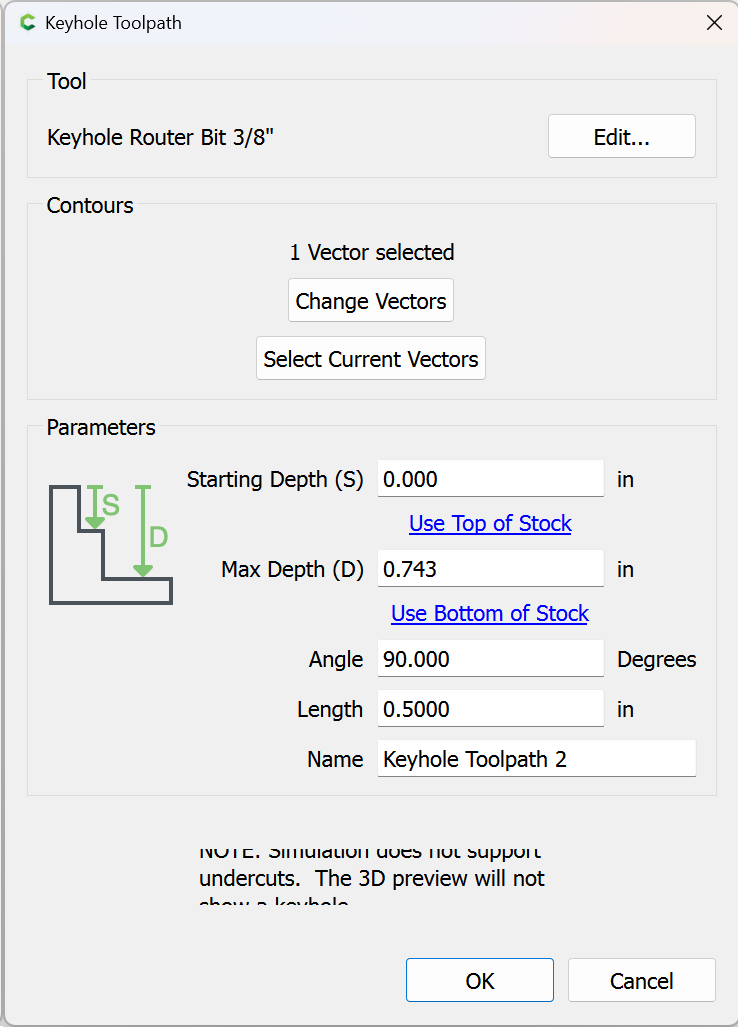
\includegraphics[width=\linewidth/2]{C:/Users/willa/OneDrive/Documents/GitHub/gcodepreview/images/cc8_dialog_toolpath_keyhole.png}\par
\end{centering}

\bigskip

\noindent Hence the parameters:

\begin{itemize}
\item Starting Depth == \verb|kh_start_depth|
\item Max Depth == \verb|kh_max_depth|
\item Angle == \verb|kht_direction|
\item Length == \verb|kh_distance|
\item Tool == \verb|kh_tool_num|
\end{itemize}

Due to the possibility of rotation, for the in-between positions there are more cases than one would think --- for each quadrant there are the following possibilities:

\begin{itemize}
 \item one node on the clockwise side is outside of the quadrant
 \item two nodes on the clockwise side are outside of the quadrant
 \item all nodes are w/in the quadrant
 \item one node on the counter-clockwise side is outside of the quadrant
 \item two nodes on the counter-clockwise side are outside of the quadrant
\end{itemize}
 
Supporting all of these would require trigonometric comparisons in the \verb|if...else| blocks, so only the 4 quadrants, N, S, E, and W will be supported in the initial version. This will be done by wrapping the command with a version which only accepts those options: 

\lstset{firstnumber=\thegcpy}
\begin{writecode}{a}{gcodepreview.py}{python}
    def cutkeyholegcdxf(self, kh_tool_num, kh_start_depth, kh_max_depth, kht_direction, kh_distance):   
        if (kht_direction == "N"): 
            toolpath = self.cutKHgcdxf(kh_tool_num, kh_start_depth, kh_max_depth, 90, kh_distance)
        elif (kht_direction == "S"):
            toolpath = self.cutKHgcdxf(kh_tool_num, kh_start_depth, kh_max_depth, 270, kh_distance)
        elif (kht_direction == "E"):
            toolpath = self.cutKHgcdxf(kh_tool_num, kh_start_depth, kh_max_depth, 0, kh_distance)
        elif (kht_direction == "W"):
            toolpath = self.cutKHgcdxf(kh_tool_num, kh_start_depth, kh_max_depth, 180, kh_distance)
        if self.generatepaths == True:
            self.toolpaths = union([self.toolpaths, toolpath])
            return toolpath
        else:
            return cube([0.01, 0.01, 0.01])

\end{writecode}
\addtocounter{gcpy}{15}

\lstset{firstnumber=\thegcpscad}
\begin{writecode}{a}{gcodepreview.scad}{scad}
module cutkeyholegcdxf(kh_tool_num, kh_start_depth, kh_max_depth, kht_direction, kh_distance){
    gcp.cutkeyholegcdxf(kh_tool_num, kh_start_depth, kh_max_depth, kht_direction, kh_distance);
}

\end{writecode}
\addtocounter{gcpscad}{4}

The original version of the command, \DescribeRoutine{cutKHgcdxf} retains an interface which allows calling it for arbitrary beginning and ending points of an arc. 

Note that code is still present for the partial calculation of one quadrant (for the case of all nodes within the quadrant). The first task is to place a circle at the origin which is invariant of angle:
 
\lstset{firstnumber=\thegcpy}
\begin{writecode}{a}{gcodepreview.py}{python}
    def cutKHgcdxf(self, kh_tool_num, kh_start_depth, kh_max_depth, kh_angle, kh_distance):
        oXpos = self.xpos()
        oYpos = self.ypos()
        self.dxfKH(kh_tool_num, self.xpos(), self.ypos(), kh_start_depth, kh_max_depth, kh_angle, kh_distance)
        toolpath = self.cutline(self.xpos(), self.ypos(), -kh_max_depth)
        self.setxpos(oXpos)
        self.setypos(oYpos)
        if self.generatepaths == False:
            return toolpath
        else: 
            return cube([0.001, 0.001, 0.001])

\end{writecode}
\addtocounter{gcpy}{12}

\lstset{firstnumber=\thegcpy}
\begin{writecode}{a}{gcodepreview.py}{python}
    def dxfKH(self, kh_tool_num, oXpos, oYpos, kh_start_depth, kh_max_depth, kh_angle, kh_distance):
#        oXpos = self.xpos()
#        oYpos = self.ypos()
#Circle at entry hole
        self.dxfarc(kh_tool_num, oXpos, oYpos, self.tool_radius(kh_tool_num, 7), 0, 90)
        self.dxfarc(kh_tool_num, oXpos, oYpos, self.tool_radius(kh_tool_num, 7), 90, 180)
        self.dxfarc(kh_tool_num, oXpos, oYpos, self.tool_radius(kh_tool_num, 7), 180, 270)
        self.dxfarc(kh_tool_num, oXpos, oYpos, self.tool_radius(kh_tool_num, 7), 270, 360)
\end{writecode}
\addtocounter{gcpy}{8}

Then it will be necessary to test for each possible case in a series of If Else blocks:
 
\lstset{firstnumber=\thegcpy}
\begin{writecode}{a}{gcodepreview.py}{python}
#pre-calculate needed values
        r = self.tool_radius(kh_tool_num, 7)
#        print(r)
        rt = self.tool_radius(kh_tool_num, 1)
#        print(rt)
        ro = math.sqrt((self.tool_radius(kh_tool_num, 1))**2-(self.tool_radius(kh_tool_num, 7))**2)
#        print(ro)
        angle = math.degrees(math.acos(ro/rt))
#Outlines of entry hole and slot
        if (kh_angle == 0):
#Lower left of entry hole
            self.dxfarc(kh_tool_num, self.xpos(), self.ypos(), self.tool_radius(kh_tool_num, 1), 180, 270)
#Upper left of entry hole
            self.dxfarc(kh_tool_num, self.xpos(), self.ypos(), self.tool_radius(kh_tool_num, 1), 90, 180)
#Upper right of entry hole
#            self.dxfarc(kh_tool_num, self.xpos(), self.ypos(), rt, 41.810, 90)
            self.dxfarc(kh_tool_num, self.xpos(), self.ypos(), rt, angle, 90)
#Lower right of entry hole
            self.dxfarc(kh_tool_num, self.xpos(), self.ypos(), rt, 270, 360-angle)
#            self.dxfarc(kh_tool_num, self.xpos(), self.ypos(), self.tool_radius(kh_tool_num, 1), 270, 270+math.acos(math.radians(self.tool_diameter(kh_tool_num, 5)/self.tool_diameter(kh_tool_num, 1))))
#Actual line of cut
#            self.dxfline(kh_tool_num, self.xpos(), self.ypos(), self.xpos()+kh_distance, self.ypos())
#upper right of end of slot (kh_max_depth+4.36))/2
            self.dxfarc(kh_tool_num, self.xpos()+kh_distance, self.ypos(), self.tool_diameter(kh_tool_num, (kh_max_depth+4.36))/2, 0, 90)
#lower right of end of slot
            self.dxfarc(kh_tool_num, self.xpos()+kh_distance, self.ypos(), self.tool_diameter(kh_tool_num, (kh_max_depth+4.36))/2, 270, 360)
#upper right slot
            self.dxfline(kh_tool_num, self.xpos()+ro, self.ypos()-(self.tool_diameter(kh_tool_num, 7)/2), self.xpos()+kh_distance, self.ypos()-(self.tool_diameter(kh_tool_num, 7)/2))
#            self.dxfline(kh_tool_num, self.xpos()+(sqrt((self.tool_diameter(kh_tool_num, 1)^2)-(self.tool_diameter(kh_tool_num, 5)^2))/2), self.ypos()+self.tool_diameter(kh_tool_num, (kh_max_depth))/2, ( (kh_max_depth-6.34))/2)^2-(self.tool_diameter(kh_tool_num, (kh_max_depth-6.34))/2)^2, self.xpos()+kh_distance, self.ypos()+self.tool_diameter(kh_tool_num, (kh_max_depth))/2, kh_tool_num)
#end position at top of slot
#lower right slot
            self.dxfline(kh_tool_num, self.xpos()+ro, self.ypos()+(self.tool_diameter(kh_tool_num, 7)/2), self.xpos()+kh_distance, self.ypos()+(self.tool_diameter(kh_tool_num, 7)/2))
#        dxfline(kh_tool_num, self.xpos()+(sqrt((self.tool_diameter(kh_tool_num, 1)^2)-(self.tool_diameter(kh_tool_num, 5)^2))/2), self.ypos()-self.tool_diameter(kh_tool_num, (kh_max_depth))/2, ( (kh_max_depth-6.34))/2)^2-(self.tool_diameter(kh_tool_num, (kh_max_depth-6.34))/2)^2, self.xpos()+kh_distance, self.ypos()-self.tool_diameter(kh_tool_num, (kh_max_depth))/2, KH_tool_num)
#end position at top of slot
#    hull(){
#      translate([xpos(), ypos(), zpos()]){
#        keyhole_shaft(6.35, 9.525);
#      }
#      translate([xpos(), ypos(), zpos()-kh_max_depth]){
#        keyhole_shaft(6.35, 9.525);
#      }
#    }
#    hull(){
#      translate([xpos(), ypos(), zpos()-kh_max_depth]){
#        keyhole_shaft(6.35, 9.525);
#      }
#      translate([xpos()+kh_distance, ypos(), zpos()-kh_max_depth]){
#        keyhole_shaft(6.35, 9.525);
#      }
#    }
#    cutwithfeed(getxpos(), getypos(), -kh_max_depth, feed);
#    cutwithfeed(getxpos()+kh_distance, getypos(), -kh_max_depth, feed);
#    setxpos(getxpos()-kh_distance);
#  } else if (kh_angle > 0 && kh_angle < 90) {
#//echo(kh_angle);
#  dxfarc(getxpos(), getypos(), tool_diameter(KH_tool_num, (kh_max_depth))/2, 90+kh_angle, 180+kh_angle, KH_tool_num);
#  dxfarc(getxpos(), getypos(), tool_diameter(KH_tool_num, (kh_max_depth))/2, 180+kh_angle, 270+kh_angle, KH_tool_num);
#dxfarc(getxpos(), getypos(), tool_diameter(KH_tool_num, (kh_max_depth))/2, kh_angle+asin((tool_diameter(KH_tool_num, (kh_max_depth+4.36))/2)/(tool_diameter(KH_tool_num, (kh_max_depth))/2)), 90+kh_angle, KH_tool_num);
#dxfarc(getxpos(), getypos(), tool_diameter(KH_tool_num, (kh_max_depth))/2, 270+kh_angle, 360+kh_angle-asin((tool_diameter(KH_tool_num, (kh_max_depth+4.36))/2)/(tool_diameter(KH_tool_num, (kh_max_depth))/2)), KH_tool_num);
#dxfarc(getxpos()+(kh_distance*cos(kh_angle)), 
#  getypos()+(kh_distance*sin(kh_angle)), tool_diameter(KH_tool_num, (kh_max_depth+4.36))/2, 0+kh_angle, 90+kh_angle, KH_tool_num);
#dxfarc(getxpos()+(kh_distance*cos(kh_angle)), getypos()+(kh_distance*sin(kh_angle)), tool_diameter(KH_tool_num, (kh_max_depth+4.36))/2, 270+kh_angle, 360+kh_angle, KH_tool_num);
#dxfline( getxpos()+tool_diameter(KH_tool_num, (kh_max_depth))/2*cos(kh_angle+asin((tool_diameter(KH_tool_num, (kh_max_depth+4.36))/2)/(tool_diameter(KH_tool_num, (kh_max_depth))/2))), 
# getypos()+tool_diameter(KH_tool_num, (kh_max_depth))/2*sin(kh_angle+asin((tool_diameter(KH_tool_num, (kh_max_depth+4.36))/2)/(tool_diameter(KH_tool_num, (kh_max_depth))/2))), 
# getxpos()+(kh_distance*cos(kh_angle))-((tool_diameter(KH_tool_num, (kh_max_depth+4.36))/2)*sin(kh_angle)), 
# getypos()+(kh_distance*sin(kh_angle))+((tool_diameter(KH_tool_num, (kh_max_depth+4.36))/2)*cos(kh_angle)), KH_tool_num);
#//echo("a", tool_diameter(KH_tool_num, (kh_max_depth+4.36))/2);
#//echo("c", tool_diameter(KH_tool_num, (kh_max_depth))/2);
#echo("Aangle", asin((tool_diameter(KH_tool_num, (kh_max_depth+4.36))/2)/(tool_diameter(KH_tool_num, (kh_max_depth))/2)));
#//echo(kh_angle);
# cutwithfeed(getxpos()+(kh_distance*cos(kh_angle)), getypos()+(kh_distance*sin(kh_angle)), -kh_max_depth, feed);
#            toolpath = toolpath.union(self.cutline(self.xpos()+kh_distance, self.ypos(), -kh_max_depth))
        elif (kh_angle == 90):
#Lower left of entry hole
            self.dxfarc(kh_tool_num, oXpos, oYpos, self.tool_radius(kh_tool_num, 1), 180, 270)
#Lower right of entry hole
            self.dxfarc(kh_tool_num, oXpos, oYpos, self.tool_radius(kh_tool_num, 1), 270, 360)
#left slot
            self.dxfline(kh_tool_num, oXpos-r, oYpos+ro, oXpos-r, oYpos+kh_distance)
#right slot
            self.dxfline(kh_tool_num, oXpos+r, oYpos+ro, oXpos+r, oYpos+kh_distance)
#upper left of end of slot
            self.dxfarc(kh_tool_num, oXpos, oYpos+kh_distance, r, 90, 180)
#upper right of end of slot
            self.dxfarc(kh_tool_num, oXpos, oYpos+kh_distance, r, 0, 90)
#Upper right of entry hole
            self.dxfarc(kh_tool_num, oXpos, oYpos, rt, 0, 90-angle)
#Upper left of entry hole
            self.dxfarc(kh_tool_num, oXpos, oYpos, rt, 90+angle, 180)
#            toolpath = toolpath.union(self.cutline(oXpos, oYpos+kh_distance, -kh_max_depth))
        elif (kh_angle == 180):
#Lower right of entry hole
            self.dxfarc(kh_tool_num, oXpos, oYpos, self.tool_radius(kh_tool_num, 1), 270, 360)
#Upper right of entry hole
            self.dxfarc(kh_tool_num, oXpos, oYpos, self.tool_radius(kh_tool_num, 1), 0, 90)
#Upper left of entry hole
            self.dxfarc(kh_tool_num, oXpos, oYpos, rt, 90, 180-angle)
#Lower left of entry hole
            self.dxfarc(kh_tool_num, oXpos, oYpos, rt, 180+angle, 270)
#upper slot
            self.dxfline(kh_tool_num, oXpos-ro, oYpos-r, oXpos-kh_distance, oYpos-r)
#lower slot
            self.dxfline(kh_tool_num, oXpos-ro, oYpos+r, oXpos-kh_distance, oYpos+r)
#upper left of end of slot
            self.dxfarc(kh_tool_num, oXpos-kh_distance, oYpos, r, 90, 180)
#lower left of end of slot
            self.dxfarc(kh_tool_num, oXpos-kh_distance, oYpos, r, 180, 270)
#            toolpath = toolpath.union(self.cutline(oXpos-kh_distance, oYpos, -kh_max_depth))
        elif (kh_angle == 270):
#Upper left of entry hole
            self.dxfarc(kh_tool_num, oXpos, oYpos, self.tool_radius(kh_tool_num, 1), 90, 180)
#Upper right of entry hole
            self.dxfarc(kh_tool_num, oXpos, oYpos, self.tool_radius(kh_tool_num, 1), 0, 90)
#left slot
            self.dxfline(kh_tool_num, oXpos-r, oYpos-ro, oXpos-r, oYpos-kh_distance)
#right slot
            self.dxfline(kh_tool_num, oXpos+r, oYpos-ro, oXpos+r, oYpos-kh_distance)
#lower left of end of slot
            self.dxfarc(kh_tool_num, oXpos, oYpos-kh_distance, r, 180, 270)
#lower right of end of slot
            self.dxfarc(kh_tool_num, oXpos, oYpos-kh_distance, r, 270, 360)
#lower right of entry hole
            self.dxfarc(kh_tool_num, oXpos, oYpos, rt, 180, 270-angle)
#lower left of entry hole
            self.dxfarc(kh_tool_num, oXpos, oYpos, rt, 270+angle, 360)
#            toolpath = toolpath.union(self.cutline(oXpos, oYpos-kh_distance, -kh_max_depth))
#        print(self.zpos())
#        self.setxpos(oXpos)
#        self.setypos(oYpos)
#        if self.generatepaths == False:
#            return toolpath
            
#  } else if (kh_angle == 90) {
#    //Lower left of entry hole
#    dxfarc(getxpos(), getypos(), 9.525/2, 180, 270, KH_tool_num);
#    //Lower right of entry hole
#    dxfarc(getxpos(), getypos(), 9.525/2, 270, 360, KH_tool_num);
#    //Upper right of entry hole
#    dxfarc(getxpos(), getypos(), 9.525/2, 0, acos(tool_diameter(KH_tool_num, 5)/tool_diameter(KH_tool_num, 1)), KH_tool_num);
#    //Upper left of entry hole
#    dxfarc(getxpos(), getypos(), 9.525/2, 180-acos(tool_diameter(KH_tool_num, 5)/tool_diameter(KH_tool_num, 1)), 180, KH_tool_num);
#    //Actual line of cut
#    dxfline(getxpos(), getypos(), getxpos(), getypos()+kh_distance);
#    //upper right of slot
#    dxfarc(getxpos(), getypos()+kh_distance, tool_diameter(KH_tool_num, (kh_max_depth+4.36))/2, 0, 90, KH_tool_num);
#    //upper left of slot
#    dxfarc(getxpos(), getypos()+kh_distance, tool_diameter(KH_tool_num, (kh_max_depth+6.35))/2, 90, 180, KH_tool_num);
#    //right of slot
#    dxfline(
#        getxpos()+tool_diameter(KH_tool_num, (kh_max_depth))/2, 
#        getypos()+(sqrt((tool_diameter(KH_tool_num, 1)^2)-(tool_diameter(KH_tool_num, 5)^2))/2), //( (kh_max_depth-6.34))/2)^2-(tool_diameter(KH_tool_num, (kh_max_depth-6.34))/2)^2, 
#        getxpos()+tool_diameter(KH_tool_num, (kh_max_depth))/2, 
#    //end position at top of slot
#        getypos()+kh_distance, 
#        KH_tool_num);
#    dxfline(getxpos()-tool_diameter(KH_tool_num, (kh_max_depth))/2, getypos()+(sqrt((tool_diameter(KH_tool_num, 1)^2)-(tool_diameter(KH_tool_num, 5)^2))/2), getxpos()-tool_diameter(KH_tool_num, (kh_max_depth+6.35))/2, getypos()+kh_distance, KH_tool_num);
#    hull(){
#      translate([xpos(), ypos(), zpos()]){
#        keyhole_shaft(6.35, 9.525);
#      }
#      translate([xpos(), ypos(), zpos()-kh_max_depth]){
#        keyhole_shaft(6.35, 9.525);
#      }
#    }
#    hull(){
#      translate([xpos(), ypos(), zpos()-kh_max_depth]){
#        keyhole_shaft(6.35, 9.525);
#      }
#      translate([xpos(), ypos()+kh_distance, zpos()-kh_max_depth]){
#        keyhole_shaft(6.35, 9.525);
#      }
#    }
#    cutwithfeed(getxpos(), getypos(), -kh_max_depth, feed);
#    cutwithfeed(getxpos(), getypos()+kh_distance, -kh_max_depth, feed);
#    setypos(getypos()-kh_distance);
#  } else if (kh_angle == 180) {
#    //Lower right of entry hole
#    dxfarc(getxpos(), getypos(), 9.525/2, 270, 360, KH_tool_num);
#    //Upper right of entry hole
#    dxfarc(getxpos(), getypos(), 9.525/2, 0, 90, KH_tool_num);
#    //Upper left of entry hole
#    dxfarc(getxpos(), getypos(), 9.525/2, 90, 90+acos(tool_diameter(KH_tool_num, 5)/tool_diameter(KH_tool_num, 1)), KH_tool_num);
#    //Lower left of entry hole
#    dxfarc(getxpos(), getypos(), 9.525/2, 270-acos(tool_diameter(KH_tool_num, 5)/tool_diameter(KH_tool_num, 1)), 270, KH_tool_num);
#    //upper left of slot
#    dxfarc(getxpos()-kh_distance, getypos(), tool_diameter(KH_tool_num, (kh_max_depth+6.35))/2, 90, 180, KH_tool_num);
#    //lower left of slot
#    dxfarc(getxpos()-kh_distance, getypos(), tool_diameter(KH_tool_num, (kh_max_depth+6.35))/2, 180, 270, KH_tool_num);
#    //Actual line of cut
#    dxfline(getxpos(), getypos(), getxpos()-kh_distance, getypos());
#    //upper left slot
#    dxfline(
#        getxpos()-(sqrt((tool_diameter(KH_tool_num, 1)^2)-(tool_diameter(KH_tool_num, 5)^2))/2), 
#        getypos()+tool_diameter(KH_tool_num, (kh_max_depth))/2, //( (kh_max_depth-6.34))/2)^2-(tool_diameter(KH_tool_num, (kh_max_depth-6.34))/2)^2, 
#        getxpos()-kh_distance, 
#    //end position at top of slot
#        getypos()+tool_diameter(KH_tool_num, (kh_max_depth))/2, 
#        KH_tool_num);
#    //lower right slot
#    dxfline(
#        getxpos()-(sqrt((tool_diameter(KH_tool_num, 1)^2)-(tool_diameter(KH_tool_num, 5)^2))/2), 
#        getypos()-tool_diameter(KH_tool_num, (kh_max_depth))/2, //( (kh_max_depth-6.34))/2)^2-(tool_diameter(KH_tool_num, (kh_max_depth-6.34))/2)^2, 
#        getxpos()-kh_distance, 
#    //end position at top of slot
#        getypos()-tool_diameter(KH_tool_num, (kh_max_depth))/2, 
#        KH_tool_num);
#    hull(){
#      translate([xpos(), ypos(), zpos()]){
#        keyhole_shaft(6.35, 9.525);
#      }
#      translate([xpos(), ypos(), zpos()-kh_max_depth]){
#        keyhole_shaft(6.35, 9.525);
#      }
#    }
#    hull(){
#      translate([xpos(), ypos(), zpos()-kh_max_depth]){
#        keyhole_shaft(6.35, 9.525);
#      }
#      translate([xpos()-kh_distance, ypos(), zpos()-kh_max_depth]){
#        keyhole_shaft(6.35, 9.525);
#      }
#    }
#    cutwithfeed(getxpos(), getypos(), -kh_max_depth, feed);
#    cutwithfeed(getxpos()-kh_distance, getypos(), -kh_max_depth, feed);
#    setxpos(getxpos()+kh_distance);
#  } else if (kh_angle == 270) {
#    //Upper right of entry hole
#    dxfarc(getxpos(), getypos(), 9.525/2, 0, 90, KH_tool_num);
#    //Upper left of entry hole
#    dxfarc(getxpos(), getypos(), 9.525/2, 90, 180, KH_tool_num);
#    //lower right of slot
#    dxfarc(getxpos(), getypos()-kh_distance, tool_diameter(KH_tool_num, (kh_max_depth+4.36))/2, 270, 360, KH_tool_num);
#    //lower left of slot
#    dxfarc(getxpos(), getypos()-kh_distance, tool_diameter(KH_tool_num, (kh_max_depth+4.36))/2, 180, 270, KH_tool_num);
#    //Actual line of cut
#    dxfline(getxpos(), getypos(), getxpos(), getypos()-kh_distance);
#    //right of slot
#    dxfline(
#        getxpos()+tool_diameter(KH_tool_num, (kh_max_depth))/2, 
#        getypos()-(sqrt((tool_diameter(KH_tool_num, 1)^2)-(tool_diameter(KH_tool_num, 5)^2))/2), //( (kh_max_depth-6.34))/2)^2-(tool_diameter(KH_tool_num, (kh_max_depth-6.34))/2)^2, 
#        getxpos()+tool_diameter(KH_tool_num, (kh_max_depth))/2, 
#    //end position at top of slot
#        getypos()-kh_distance, 
#        KH_tool_num);
#    //left of slot
#    dxfline(
#        getxpos()-tool_diameter(KH_tool_num, (kh_max_depth))/2, 
#        getypos()-(sqrt((tool_diameter(KH_tool_num, 1)^2)-(tool_diameter(KH_tool_num, 5)^2))/2), //( (kh_max_depth-6.34))/2)^2-(tool_diameter(KH_tool_num, (kh_max_depth-6.34))/2)^2, 
#        getxpos()-tool_diameter(KH_tool_num, (kh_max_depth))/2, 
#    //end position at top of slot
#        getypos()-kh_distance, 
#        KH_tool_num);
#    //Lower right of entry hole
#    dxfarc(getxpos(), getypos(), 9.525/2, 360-acos(tool_diameter(KH_tool_num, 5)/tool_diameter(KH_tool_num, 1)), 360, KH_tool_num);
#    //Lower left of entry hole
#    dxfarc(getxpos(), getypos(), 9.525/2, 180, 180+acos(tool_diameter(KH_tool_num, 5)/tool_diameter(KH_tool_num, 1)), KH_tool_num);
#    hull(){
#      translate([xpos(), ypos(), zpos()]){
#        keyhole_shaft(6.35, 9.525);
#      }
#      translate([xpos(), ypos(), zpos()-kh_max_depth]){
#        keyhole_shaft(6.35, 9.525);
#      }
#    }
#    hull(){
#      translate([xpos(), ypos(), zpos()-kh_max_depth]){
#        keyhole_shaft(6.35, 9.525);
#      }
#      translate([xpos(), ypos()-kh_distance, zpos()-kh_max_depth]){
#        keyhole_shaft(6.35, 9.525);
#      }
#    }
#    cutwithfeed(getxpos(), getypos(), -kh_max_depth, feed);
#    cutwithfeed(getxpos(), getypos()-kh_distance, -kh_max_depth, feed);
#    setypos(getypos()+kh_distance);
#  }
#}

\end{writecode}
\addtocounter{gcpy}{278}

\subparagraph*{Dovetail joinery and tooling}
 
\label{subsec:dovetails}

One focus of this project from the beginning has been cutting joinery. The first such toolpath to be developed is half-blind dovetails, since they are intrinsically simple to calculate since their geometry is dictated by the geometry of the tool.

BlocksCAD project page at: \url{https://www.blockscad3d.com/community/projects/1941456} and discussion at: \url{https://community.carbide3d.com/t/tool-paths-for-different-sized-dovetail-bits/89098}

Making such cuts will require dovetail tooling such as:

\begin{itemize}
\item 808079  \url{https://www.amanatool.com/45828-carbide-tipped-dovetail-8-deg-x-1-2-dia-x-825-x-1-4-inch-shank.html}
\item 814  \url{https://www.leevalley.com/en-us/shop/tools/power-tool-accessories/router-bits/30172-dovetail-bits?item=18J1607}
\end{itemize}

Two commands are required:

\lstset{firstnumber=\thegcpy}
\begin{writecode}{a}{gcodepreview.py}{python}
    def cut_pins(self, Joint_Width, stockZthickness, Number_of_Dovetails, Spacing, Proportion, DTT_diameter, DTT_angle):
        DTO = math.tan(math.radians(DTT_angle)) * (stockZthickness * Proportion)
        DTR = DTT_diameter/2 - DTO
        cpr = self.rapidXY(0, stockZthickness + Spacing/2)
        ctp = self.cutlinedxfgc(self.xpos(), self.ypos(), -stockZthickness * Proportion)
#        ctp = ctp.union(self.cutlinedxfgc(Joint_Width / (Number_of_Dovetails * 2), self.ypos(), -stockZthickness * Proportion))
        i = 1
        while i < Number_of_Dovetails * 2:
#            print(i)
            ctp = ctp.union(self.cutlinedxfgc(i * (Joint_Width / (Number_of_Dovetails * 2)), self.ypos(), -stockZthickness * Proportion))
            ctp = ctp.union(self.cutlinedxfgc(i * (Joint_Width / (Number_of_Dovetails * 2)), (stockZthickness + Spacing) + (stockZthickness * Proportion) - (DTT_diameter/2), -(stockZthickness * Proportion)))
            ctp = ctp.union(self.cutlinedxfgc(i * (Joint_Width / (Number_of_Dovetails * 2)), stockZthickness + Spacing/2, -(stockZthickness * Proportion)))
            ctp = ctp.union(self.cutlinedxfgc((i + 1) * (Joint_Width / (Number_of_Dovetails * 2)), stockZthickness + Spacing/2,-(stockZthickness * Proportion)))
            self.dxfrectangleround(self.currenttoolnumber(), 
                i * (Joint_Width / (Number_of_Dovetails * 2))-DTR, 
                stockZthickness + (Spacing/2) - DTR, 
                DTR * 2,
                (stockZthickness * Proportion) + Spacing/2 + DTR * 2 - (DTT_diameter/2), 
                DTR)
            i += 2
        self.rapidZ(0)
        return ctp
    
\end{writecode}
\addtocounter{gcpy}{23}

\noindent and

\lstset{firstnumber=\thegcpy}
\begin{writecode}{a}{gcodepreview.py}{python}
    def cut_tails(self, Joint_Width, stockZthickness, Number_of_Dovetails, Spacing, Proportion, DTT_diameter, DTT_angle):
        DTO = math.tan(math.radians(DTT_angle)) * (stockZthickness * Proportion)
        DTR = DTT_diameter/2 - DTO
        cpr = self.rapidXY(0, 0)
        ctp = self.cutlinedxfgc(self.xpos(), self.ypos(), -stockZthickness * Proportion)
        ctp = ctp.union(self.cutlinedxfgc(
            Joint_Width / (Number_of_Dovetails * 2) - (DTT_diameter - DTO), 
            self.ypos(), 
            -stockZthickness * Proportion))
        i = 1
        while i < Number_of_Dovetails * 2:
            ctp = ctp.union(self.cutlinedxfgc(
                i * (Joint_Width / (Number_of_Dovetails * 2)) - (DTT_diameter - DTO), 
                stockZthickness * Proportion - DTT_diameter / 2,
                -(stockZthickness * Proportion)))
            ctp = ctp.union(self.cutarcCWdxf(180, 90, 
                i * (Joint_Width / (Number_of_Dovetails * 2)), 
                stockZthickness * Proportion - DTT_diameter / 2,
#                self.ypos(), 
                DTT_diameter - DTO,  0, 1))
            ctp = ctp.union(self.cutarcCWdxf(90, 0, 
                i * (Joint_Width / (Number_of_Dovetails * 2)), 
                stockZthickness * Proportion - DTT_diameter / 2, 
                DTT_diameter - DTO,  0, 1))
            ctp = ctp.union(self.cutlinedxfgc(
                i * (Joint_Width / (Number_of_Dovetails * 2)) + (DTT_diameter - DTO), 
                0, 
                -(stockZthickness * Proportion)))
            ctp = ctp.union(self.cutlinedxfgc(
                (i + 2) * (Joint_Width / (Number_of_Dovetails * 2)) - (DTT_diameter - DTO), 
                0, 
                -(stockZthickness * Proportion)))
            i += 2
        self.rapidZ(0)
        self.rapidXY(0, 0)
        ctp = ctp.union(self.cutlinedxfgc(self.xpos(), self.ypos(), -stockZthickness * Proportion))
        self.dxfarc(self.currenttoolnumber(), 0, 0, DTR, 180, 270)
        self.dxfline(self.currenttoolnumber(), -DTR, 0, -DTR, stockZthickness + DTR)
        self.dxfarc(self.currenttoolnumber(), 0, stockZthickness + DTR, DTR, 90, 180)
        self.dxfline(self.currenttoolnumber(), 0, stockZthickness + DTR * 2, Joint_Width, stockZthickness + DTR * 2)
        i = 0
        while i < Number_of_Dovetails * 2:
            ctp = ctp.union(self.cutline(i * (Joint_Width / (Number_of_Dovetails * 2)), stockZthickness + DTO, -(stockZthickness * Proportion)))
            ctp = ctp.union(self.cutline((i+2) * (Joint_Width / (Number_of_Dovetails * 2)), stockZthickness + DTO, -(stockZthickness * Proportion)))
            ctp = ctp.union(self.cutline((i+2) * (Joint_Width / (Number_of_Dovetails * 2)), 0, -(stockZthickness * Proportion)))
            self.dxfarc(self.currenttoolnumber(), i * (Joint_Width / (Number_of_Dovetails * 2)), 0, DTR, 270, 360)
            self.dxfline(self.currenttoolnumber(), 
                i * (Joint_Width / (Number_of_Dovetails * 2)) + DTR, 
                0, 
                i * (Joint_Width / (Number_of_Dovetails * 2)) + DTR, stockZthickness * Proportion - DTT_diameter / 2)
            self.dxfarc(self.currenttoolnumber(), (i + 1) * (Joint_Width / (Number_of_Dovetails * 2)), stockZthickness * Proportion - DTT_diameter / 2, (Joint_Width / (Number_of_Dovetails * 2)) - DTR, 90, 180)
            self.dxfarc(self.currenttoolnumber(), (i + 1) * (Joint_Width / (Number_of_Dovetails * 2)), stockZthickness * Proportion - DTT_diameter / 2, (Joint_Width / (Number_of_Dovetails * 2)) - DTR, 0, 90)
            self.dxfline(self.currenttoolnumber(), 
                (i + 2) * (Joint_Width / (Number_of_Dovetails * 2)) - DTR, 
                0, 
                (i + 2) * (Joint_Width / (Number_of_Dovetails * 2)) - DTR, stockZthickness * Proportion - DTT_diameter / 2)
            self.dxfarc(self.currenttoolnumber(), (i + 2) * (Joint_Width / (Number_of_Dovetails * 2)), 0, DTR, 180, 270)
            i += 2
        self.dxfarc(self.currenttoolnumber(), Joint_Width, stockZthickness + DTR, DTR, 0, 90)
        self.dxfline(self.currenttoolnumber(), Joint_Width + DTR, stockZthickness + DTR, Joint_Width + DTR, 0)
        self.dxfarc(self.currenttoolnumber(), Joint_Width, 0, DTR, 270, 360)
        return ctp

\end{writecode}
\addtocounter{gcpy}{63}

\noindent which are used as:

\begin{verbatim}
toolpaths = gcp.cut_pins(stockXwidth, stockZthickness, Number_of_Dovetails, Spacing, Proportion, DTT_diameter, DTT_angle)

toolpaths = toolpaths.union(gcp.cut_tails(stockXwidth, stockZthickness, Number_of_Dovetails, Spacing, Proportion, DTT_diameter, DTT_angle))
\end{verbatim}

Future versions may adjust the parameters passed in, having them calculate from the specifications for the currently active dovetail tool.

\subparagraph*{Full-blind box joints}
 
\label{subsec:fullblindboxjoints}

BlocksCAD project page at: \url{https://www.blockscad3d.com/community/projects/1943966} and discussion at: \url{https://community.carbide3d.com/t/full-blind-box-joints-in-carbide-create/53329}

Full-blind box joints will require 3 separate tools:

\begin{itemize}
\item small V tool --- this will be needed to make a cut along the edge of the joint
\item small square tool --- this should be the same diameter as the small V tool
\item large V tool --- this will facilitate the stock being of a greater thickness and avoid the need to make multiple cuts to cut the blind miters at the ends of the joint
\end{itemize}

Two different versions of the commands will be necessary, one for each orientation:

\begin{itemize}
\item horizontal
\item vertical
\end{itemize}

\noindent and then the internal commands for each side will in turn need separate versions:

\lstset{firstnumber=\thegcpy}
\begin{writecode}{a}{gcodepreview.py}{python}
    def Full_Blind_Finger_Joint(self, bx, by, orientation, side, width, thickness, largeVdiameter, smallDiameter, normalormirror = "Default", squaretool = 102, smallV = 390, largeV = 301):
        Number_of_Pins = int(((width - thickness * 2) / (smallDiameter * 2.2) / 2) + 0.0) * 2 + 1
#        print("Number of Pins: ",Number_of_Pins)
        self.movetosafeZ()
        self.toolchange(squaretool, 17000)
        toolpath = self.Full_Blind_Finger_Joint_square(bx, by, orientation, side, width, thickness, Number_of_Pins, largeVdiameter, smallDiameter)
        self.movetosafeZ()
        self.toolchange(smallV, 17000)
        toolpath = toolpath.union(self.Full_Blind_Finger_Joint_smallV(bx, by, orientation, side, width, thickness, Number_of_Pins, largeVdiameter, smallDiameter))
        self.toolchange(largeV, 17000)
        toolpath = toolpath.union(self.Full_Blind_Finger_Joint_largeV(bx, by, orientation, side, width, thickness, Number_of_Pins, largeVdiameter, smallDiameter))
        return toolpath

    def Full_Blind_Finger_Joint_square(self, bx, by, orientation, side, width, thickness, Number_of_Pins, largeVdiameter, smallDiameter, normalormirror = "Default"):
#     Joint_Orientation = "Horizontal" "Even" == "Lower", "Odd" == "Upper"
#     Joint_Orientation = "Vertical" "Even" == "Left", "Odd" == "Right"
        if (orientation == "Vertical"):
            if (normalormirror == "Default" and side != "Both"):
                if (side == "Left"):
                    normalormirror = "Even"
                if (side == "Right"):
                    normalormirror = "Odd"
        if (orientation == "Horizontal"):
            if (normalormirror == "Default" and side != "Both"):
                if (side == "Lower"):
                    normalormirror = "Even"
                if (side == "Upper"):
                    normalormirror = "Odd"
        Finger_Width = ((Number_of_Pins * 2) - 1) * smallDiameter * 1.1
        Finger_Origin = width/2 - Finger_Width/2
        rapid = self.rapidZ(0)
        self.setdxfcolor("Cyan")
        rapid = rapid.union(self.rapidXY(bx, by))
        toolpath = (self.Finger_Joint_square(bx, by, orientation, side, width, thickness, Number_of_Pins, Finger_Origin, smallDiameter))
        if (orientation == "Vertical"):
            if (side == "Both"):
                toolpath = self.cutrectanglerounddxf(self.currenttoolnum, bx - (thickness - smallDiameter/2), by-smallDiameter/2, 0, (thickness * 2) - smallDiameter, width+smallDiameter, (smallDiameter / 2) / math.tan(math.radians(45)), smallDiameter/2)
            if (side == "Left"):
                toolpath = self.cutrectanglerounddxf(self.currenttoolnum, bx - (smallDiameter/2), by-smallDiameter/2, 0, thickness, width+smallDiameter, ((smallDiameter / 2) / math.tan(math.radians(45))), smallDiameter/2)
            if (side == "Right"):
                toolpath = self.cutrectanglerounddxf(self.currenttoolnum, bx - (thickness - smallDiameter/2), by-smallDiameter/2, 0, thickness, width+smallDiameter, ((smallDiameter / 2) / math.tan(math.radians(45))), smallDiameter/2)
        toolpath = toolpath.union(self.Finger_Joint_square(bx, by, orientation, side, width, thickness, Number_of_Pins, Finger_Origin, smallDiameter))
        if (orientation == "Horizontal"):
            if (side == "Both"):
                toolpath = self.cutrectanglerounddxf(
                    self.currenttoolnum, 
                    bx-smallDiameter/2, 
                    by - (thickness - smallDiameter/2), 
                    0, 
                    width+smallDiameter, 
                    (thickness * 2) - smallDiameter, 
                    (smallDiameter / 2) / math.tan(math.radians(45)), 
                    smallDiameter/2)
            if (side == "Lower"):
                toolpath = self.cutrectanglerounddxf(
                    self.currenttoolnum, 
                    bx - (smallDiameter/2), 
                    by - smallDiameter/2, 
                    0, 
                    width+smallDiameter, 
                    thickness, 
                    ((smallDiameter / 2) / math.tan(math.radians(45))), 
                    smallDiameter/2)
            if (side == "Upper"):
                toolpath = self.cutrectanglerounddxf(
                    self.currenttoolnum, 
                    bx - smallDiameter/2, 
                    by - (thickness - smallDiameter/2), 
                    0, 
                    width+smallDiameter, 
                    thickness, 
                    ((smallDiameter / 2) / math.tan(math.radians(45))), 
                    smallDiameter/2)
        toolpath = toolpath.union(self.Finger_Joint_square(bx, by, orientation, side, width, thickness, Number_of_Pins, Finger_Origin, smallDiameter))
        return toolpath

    def Finger_Joint_square(self, bx, by, orientation, side, width, thickness, Number_of_Pins, Finger_Origin, smallDiameter, normalormirror = "Default"):
        jointdepth = -(thickness - (smallDiameter / 2) / math.tan(math.radians(45)))
    # Joint_Orientation = "Horizontal" "Even" == "Lower", "Odd" == "Upper"
    # Joint_Orientation = "Vertical" "Even" == "Left", "Odd" == "Right"
        if (orientation == "Vertical"):
            if (normalormirror == "Default" and side != "Both"):
                if (side == "Left"):
                     normalormirror = "Even"
                if (side == "Right"):
                     normalormirror = "Odd"
        if (orientation == "Horizontal"):
            if (normalormirror == "Default" and side != "Both"):
                if (side == "Lower"):
                     normalormirror = "Even"
                if (side == "Upper"):
                     normalormirror = "Odd"
        radius = smallDiameter/2
        jointwidth = thickness - smallDiameter
        toolpath = self.currenttool()
        rapid = self.rapidZ(0)
        self.setdxfcolor("Blue")
        toolpath = toolpath.union(self.cutlineZgcfeed(jointdepth,1000))
        self.beginpolyline(self.currenttool())
        if (orientation == "Vertical"):
            rapid = rapid.union(self.rapidXY(bx, by + Finger_Origin))
            self.addvertex(self.currenttoolnumber(), self.xpos(), self.ypos())
            toolpath = toolpath.union(self.cutlineZgcfeed(jointdepth,1000))
            i = 0
            while i <= Number_of_Pins - 1:
                if (side == "Right"):
                    toolpath = toolpath.union(self.cutvertexdxf(self.xpos(), self.ypos() + smallDiameter + radius/5, jointdepth))
                if (side == "Left" or side == "Both"):
                    toolpath = toolpath.union(self.cutvertexdxf(self.xpos(), self.ypos() + radius, jointdepth))
                    toolpath = toolpath.union(self.cutvertexdxf(self.xpos() + jointwidth, self.ypos(), jointdepth))
                    toolpath = toolpath.union(self.cutvertexdxf(self.xpos(), self.ypos() + radius/5, jointdepth))
                    toolpath = toolpath.union(self.cutvertexdxf(self.xpos() - jointwidth, self.ypos(), jointdepth))
                    toolpath = toolpath.union(self.cutvertexdxf(self.xpos(), self.ypos() + radius, jointdepth))
                if (side == "Left"):
                    toolpath = toolpath.union(self.cutvertexdxf(self.xpos(), self.ypos() + smallDiameter + radius/5, jointdepth))
                if (side == "Right" or side == "Both"):
                    if (i < (Number_of_Pins - 1)):
    #                    print(i)
                        toolpath = toolpath.union(self.cutvertexdxf(self.xpos(), self.ypos() + radius, jointdepth))
                        toolpath = toolpath.union(self.cutvertexdxf(self.xpos() - jointwidth, self.ypos(), jointdepth))
                        toolpath = toolpath.union(self.cutvertexdxf(self.xpos(), self.ypos() + radius/5, jointdepth))
                        toolpath = toolpath.union(self.cutvertexdxf(self.xpos() + jointwidth, self.ypos(), jointdepth))
                        toolpath = toolpath.union(self.cutvertexdxf(self.xpos(), self.ypos() + radius, jointdepth))
                i += 1
    # Joint_Orientation = "Horizontal" "Even" == "Lower", "Odd" == "Upper"
        if (orientation == "Horizontal"):
            rapid = rapid.union(self.rapidXY(bx + Finger_Origin, by))
            self.addvertex(self.currenttoolnumber(), self.xpos(), self.ypos())
            toolpath = toolpath.union(self.cutlineZgcfeed(jointdepth,1000))
            i = 0
            while i <= Number_of_Pins - 1:
                if (side == "Upper"):
                    toolpath = toolpath.union(self.cutvertexdxf(self.xpos() + smallDiameter + radius/5, self.ypos(), jointdepth))
                if (side == "Lower" or side == "Both"):
                    toolpath = toolpath.union(self.cutvertexdxf(self.xpos() + radius, self.ypos(), jointdepth))
                    toolpath = toolpath.union(self.cutvertexdxf(self.xpos(), self.ypos() + jointwidth, jointdepth))
                    toolpath = toolpath.union(self.cutvertexdxf(self.xpos() + radius/5, self.ypos(), jointdepth))
                    toolpath = toolpath.union(self.cutvertexdxf(self.xpos(), self.ypos() - jointwidth, jointdepth))
                    toolpath = toolpath.union(self.cutvertexdxf(self.xpos() + radius, self.ypos(), jointdepth))
                if (side == "Lower"):
                    toolpath = toolpath.union(self.cutvertexdxf(self.xpos() + smallDiameter + radius/5, self.ypos(), jointdepth))
                if (side == "Upper" or side == "Both"):
                    if (i < (Number_of_Pins - 1)):
    #                    print(i)
                        toolpath = toolpath.union(self.cutvertexdxf(self.xpos() + radius, self.ypos(), jointdepth))
                        toolpath = toolpath.union(self.cutvertexdxf(self.xpos(), self.ypos() - jointwidth, jointdepth))
                        toolpath = toolpath.union(self.cutvertexdxf(self.xpos() + radius/5, self.ypos(), jointdepth))
                        toolpath = toolpath.union(self.cutvertexdxf(self.xpos(), self.ypos() + jointwidth, jointdepth))
                        toolpath = toolpath.union(self.cutvertexdxf(self.xpos() + radius, self.ypos(), jointdepth))
                i += 1
        self.closepolyline(self.currenttoolnumber())
        return toolpath

    def Full_Blind_Finger_Joint_smallV(self, bx, by, orientation, side, width, thickness, Number_of_Pins, largeVdiameter, smallDiameter):
        rapid = self.rapidZ(0)
#        rapid = rapid.union(self.rapidXY(bx, by))
        self.setdxfcolor("Red")
        if (orientation == "Vertical"):
            rapid = rapid.union(self.rapidXY(bx, by - smallDiameter/6))
            toolpath = self.cutlineZgcfeed(-thickness,1000)
            toolpath = self.cutlinedxfgc(bx, by + width + smallDiameter/6, - thickness)
        if (orientation == "Horizontal"):
            rapid = rapid.union(self.rapidXY(bx - smallDiameter/6, by))
            toolpath = self.cutlineZgcfeed(-thickness,1000)
            toolpath = self.cutlinedxfgc(bx + width - smallDiameter/6, by, -thickness)
#            rapid = self.rapidZ(0)  
        return toolpath

    def Full_Blind_Finger_Joint_largeV(self, bx, by, orientation, side, width, thickness, Number_of_Pins, largeVdiameter, smallDiameter):
        radius = smallDiameter/2
        rapid = self.rapidZ(0)
#        rapid = rapid.union(self.rapidXY(bx, by))
#     Joint_Orientation = "Horizontal" "Even" == "Lower", "Odd" == "Upper"
#     Joint_Orientation = "Vertical" "Even" == "Left", "Odd" == "Right"
        if (orientation == "Vertical"):
            rapid = rapid.union(self.rapidXY(bx, by))
            toolpath = self.cutlineZgcfeed(-thickness,1000)
            toolpath = toolpath.union(self.cutlinedxfgc(bx, by + thickness, -thickness))
            rapid = self.rapidZ(0)
            rapid = rapid.union(self.rapidXY(bx, by + width - thickness))
            self.setdxfcolor("Blue")
            toolpath = toolpath.union(self.cutlineZgcfeed(-thickness,1000))
            toolpath = toolpath.union(self.cutlinedxfgc(bx, by + width, -thickness))
            if (side == "Left" or side == "Both"):
                rapid = self.rapidZ(0)
                self.setdxfcolor("Dark Gray")
                rapid = rapid.union(self.rapidXY(bx+thickness-(smallDiameter / 2) / math.tan(math.radians(45)), by - radius/2))
                toolpath = toolpath.union(self.cutlineZgcfeed(-(smallDiameter / 2) / math.tan(math.radians(45)),10000))
                toolpath = toolpath.union(self.cutlinedxfgc(bx+thickness-(smallDiameter / 2) / math.tan(math.radians(45)), by + width + radius/2, -(smallDiameter / 2) / math.tan(math.radians(45))))
                rapid = self.rapidZ(0)
                self.setdxfcolor("Green")
                rapid = rapid.union(self.rapidXY(bx+thickness/2, by+width))
                toolpath = toolpath.union(self.cutlineZgcfeed(-thickness/2,1000))
                toolpath = toolpath.union(self.cutlinedxfgc(bx+thickness/2, by + width -thickness, -thickness/2))
                rapid = self.rapidZ(0)
                rapid = rapid.union(self.rapidXY(bx+thickness/2, by))
                toolpath = toolpath.union(self.cutlineZgcfeed(-thickness/2,1000))
                toolpath = toolpath.union(self.cutlinedxfgc(bx+thickness/2, by +thickness, -thickness/2))
            if (side == "Right" or side == "Both"):
                rapid = self.rapidZ(0)
                self.setdxfcolor("Dark Gray")
                rapid = rapid.union(self.rapidXY(bx-(thickness-(smallDiameter / 2) / math.tan(math.radians(45))), by - radius/2))
                toolpath = toolpath.union(self.cutlineZgcfeed(-(smallDiameter / 2) / math.tan(math.radians(45)),10000))
                toolpath = toolpath.union(self.cutlinedxfgc(bx-(thickness-(smallDiameter / 2) / math.tan(math.radians(45))), by + width + radius/2, -(smallDiameter / 2) / math.tan(math.radians(45))))
                rapid = self.rapidZ(0)
                self.setdxfcolor("Green")
                rapid = rapid.union(self.rapidXY(bx-thickness/2, by+width))
                toolpath = toolpath.union(self.cutlineZgcfeed(-thickness/2,1000))
                toolpath = toolpath.union(self.cutlinedxfgc(bx-thickness/2, by + width -thickness, -thickness/2))
                rapid = self.rapidZ(0)
                rapid = rapid.union(self.rapidXY(bx-thickness/2, by))
                toolpath = toolpath.union(self.cutlineZgcfeed(-thickness/2,1000))
                toolpath = toolpath.union(self.cutlinedxfgc(bx-thickness/2, by +thickness, -thickness/2))
#     Joint_Orientation = "Horizontal" "Even" == "Lower", "Odd" == "Upper"
        if (orientation == "Horizontal"):
            rapid = rapid.union(self.rapidXY(bx, by))
            self.setdxfcolor("Blue")
            toolpath = self.cutlineZgcfeed(-thickness,1000)
            toolpath = toolpath.union(self.cutlinedxfgc(bx + thickness, by, -thickness))
            rapid = rapid.union(self.rapidZ(0))
            rapid = rapid.union(self.rapidXY(bx + width - thickness, by))
            toolpath = toolpath.union(self.cutlineZgcfeed(-thickness,1000))
            toolpath = toolpath.union(self.cutlinedxfgc(bx + width, by, -thickness))
            if (side == "Lower" or side == "Both"):
                rapid = self.rapidZ(0)
                self.setdxfcolor("Dark Gray")
                rapid = rapid.union(self.rapidXY(bx - radius, by+thickness-(smallDiameter / 2) / math.tan(math.radians(45))))
                toolpath = toolpath.union(self.cutlineZgcfeed(-(smallDiameter / 2) / math.tan(math.radians(45)),10000))
                toolpath = toolpath.union(self.cutlinedxfgc(bx + width + radius, by+thickness-(smallDiameter / 2) / math.tan(math.radians(45)), -(smallDiameter / 2) / math.tan(math.radians(45))))
                rapid = self.rapidZ(0)
                self.setdxfcolor("Green")
                rapid = rapid.union(self.rapidXY(bx+width, by+thickness/2))
                toolpath = toolpath.union(self.cutlineZgcfeed(-thickness/2,1000))
                toolpath = toolpath.union(self.cutlinedxfgc(bx + width -thickness, by+thickness/2, -thickness/2))
                rapid = self.rapidZ(0)
                rapid = rapid.union(self.rapidXY(bx, by+thickness/2))
                toolpath = toolpath.union(self.cutlineZgcfeed(-thickness/2,1000))
                toolpath = toolpath.union(self.cutlinedxfgc(bx +thickness, by+thickness/2, -thickness/2))
            if (side == "Upper" or side == "Both"):
                rapid = self.rapidZ(0)
                self.setdxfcolor("Dark Gray")
                rapid = rapid.union(self.rapidXY(bx - radius, by-(thickness-(smallDiameter / 2) / math.tan(math.radians(45)))))
                toolpath = toolpath.union(self.cutlineZgcfeed(-(smallDiameter / 2) / math.tan(math.radians(45)),10000))
                toolpath = toolpath.union(self.cutlinedxfgc(bx + width + radius, by-(thickness-(smallDiameter / 2) / math.tan(math.radians(45))), -(smallDiameter / 2) / math.tan(math.radians(45))))
                rapid = self.rapidZ(0)
                self.setdxfcolor("Green")
                rapid = rapid.union(self.rapidXY(bx+width, by-thickness/2))
                toolpath = toolpath.union(self.cutlineZgcfeed(-thickness/2,1000))
                toolpath = toolpath.union(self.cutlinedxfgc(bx + width -thickness, by-thickness/2, -thickness/2))
                rapid = self.rapidZ(0)
                rapid = rapid.union(self.rapidXY(bx, by-thickness/2))
                toolpath = toolpath.union(self.cutlineZgcfeed(-thickness/2,1000))
                toolpath = toolpath.union(self.cutlinedxfgc(bx +thickness, by-thickness/2, -thickness/2))
        rapid = self.rapidZ(0)
        return toolpath
    
\end{writecode}
\addtocounter{gcpy}{179}

\subsubsection{Difference of Stock, Rapids, and Toolpaths}

At the end of cutting it will be necessary to subtract the accumulated toolpaths and rapids from the stock. If in OpenSCAD, the \textsc{3d} model is returned by each operation, causing it to be instantiated on the \textsc{3d} stage unless the Boolean \verb|generatepaths| is True.

\lstset{firstnumber=\thegcpy}
\begin{writecode}{a}{gcodepreview.py}{python}
    def stockandtoolpaths(self, option = "stockandtoolpaths"):
        if option == "stock":
            if self.generatepaths == False:
                show(self.stock)
#                print("Outputting stock")
            else:
                return self.stock
        elif option == "toolpaths":
            if self.generatepaths == False:
                show(self.toolpaths)
            else:
                return self.toolpaths
        elif option == "rapids":
            if self.generatepaths == False:
                show(self.rapids)
            else:
                return self.rapids
        else:
            part = self.stock.difference(self.toolpaths)
            if self.generatepaths == False:
                show(part)
            else:
                return part
                    
\end{writecode}
\addtocounter{gcpy}{24}

It is convenient to have specific commands reflecting the possible options:

\lstset{firstnumber=\thegcpscad}
\begin{writecode}{a}{gcodepreview.scad}{scad}
module stockandtoolpaths(){
    gcp.stockandtoolpaths();
}

module stockwotoolpaths(){
    gcp.stockandtoolpaths("stock");
}

module outputtoolpaths(){
    gcp.stockandtoolpaths("toolpaths");
}

module outputrapids(){
    gcp.stockandtoolpaths("rapids");
}

\end{writecode}
\addtocounter{gcpscad}{16}

\subsection{Output files}

The \verb|gcodepreview| class will write out \textsc{dxf} and/or G-code files.

\subsubsection{G-code Overview}
 
The G-code commands and their matching modules may include (but are not limited to):

\bigskip

\noindent \begin{tabular}{@{}ll@{}} \toprule
 Command/Module                    & G-code                                        \\ \midrule
 \texttt{opengcodefile(s)(...);}
 \texttt{setupstock(...)}          & \texttt{(export.nc)}                          \\
                                   & \texttt{(stockMin: -109.5, -75mm, -8.35mm)}\\
                                   & \texttt{(stockMax:109.5mm, 75mm, 0.00mm)}\\
                                   & \texttt{(STOCK/BLOCK, 219, 150, 8.35, 109.5, 75, 8.35)}\\
                                   & \texttt{G90}\\
                                   & \texttt{G21} \\ \midrule
 \texttt{movetosafez()}            & \texttt{(Move to safe Z to avoid workholding)}\\
                                   & \texttt{G53G0Z-5.000}\\ \midrule
 \texttt{toolchange(...);}         & \texttt{(TOOL/MILL, 3.17, 0.00, 0.00, 0.00)} \\
                                   & \texttt{M6T102} \\
                                   & \texttt{M03S16000} \\ \midrule
 \verb|cutoneaxis_setfeed(...);|   & \texttt{(PREPOSITION FOR RAPID PLUNGE)}\\
  & \texttt{G0X0Y0} \\
  & \texttt{Z0.25} \\
  & \texttt{G1Z0F100} \\
  & \texttt{G1 X109.5 Y75 Z-8.35F400} \\
  & \texttt{Z9}\\
 \texttt{cutwithfeed(...);}\\ \midrule

 \texttt{closegcodefile();}        & \texttt{M05}\\
                                   & \texttt{M02}\\ 
\bottomrule
\end{tabular}
\bigskip

\noindent Conversely, the G-code commands which are supported are generated by the following modules:

\bigskip

\noindent \begin{tabular}{@{}ll@{}} \toprule
 G-code                                                           & Command/Module \\ \midrule
 \verb|(Design File: )| &  \texttt{opengcodefile(s)(...);}
                           \texttt{setupstock(...)}\\
 \verb|(stockMin:0.00mm, -152.40mm, -34.92mm)| \\
 \verb|(stockMax:109.50mm, -77.40mm, 0.00mm)| \\
 \verb|(STOCK/BLOCK, 109.50, 75.00, 34.92, 0.00, 152.40, 34.92)| \\
 \verb|G90| \\
 \verb|G21| \\ \midrule
 \verb|(Move to safe Z to avoid workholding)| &  \texttt{movetosafez()} \\
 \verb|G53G0Z-5.000| \\ \midrule
 \verb|(Toolpath: Contour Toolpath 1)| &  \texttt{toolchange(...);}\\
 \verb|M05| \\
 \verb|(TOOL/MILL, 3.17, 0.00, 0.00, 0.00)| \\
 \verb|M6T102| \\
 \verb|M03S10000|  \\ \midrule
 \verb|(PREPOSITION FOR RAPID PLUNGE)| & \texttt{writecomment(...)}\\ \midrule
 \verb|G0X0.000Y-152.400| & \texttt{rapid(...)}\\
 \verb|Z0.250| & \texttt{rapid(...)}\\ \midrule
 \verb|G1Z-1.000F203.2| & \texttt{cutwithfeed(...);}\\  
 \verb|X109.500Y-77.400F508.0| & \texttt{cutwithfeed(...);} \\ 
 \verb|X57.918Y16.302Z-0.726|\\ 
 \verb|Y22.023Z-1.023|\\ 
 \verb|X61.190Z-0.681|\\ 
 \verb|Y21.643|\\ 
 \verb|X57.681|\\
 \verb|Z12.700|\\ \midrule
 \verb|M05| &  \texttt{closegcodefile();}\\
 \verb|M02|\\
 \bottomrule
 \end{tabular}
\bigskip

The implication here is that it should be possible to read in a G-code file, and for each line/\allowbreak command instantiate a matching command so as to create a \textsc{3d} model/preview  of the file. This is addressed by making specialized commands for movement which correspond to the various axis combinations (\textsc{xyz}, \textsc{xy}, \textsc{xz}, \textsc{yz}, \textsc{x}, \textsc{y}, \textsc{z}).

A further consideration is that rather than hard-coding all possibilities or any changes, having an option for a "post-processor" will be far more flexible.

Described at: \url{https://carbide3d.com/hub/faq/create-pro-custom-post-processor/} the necessary hooks would be:

\begin{itemize}
\item onOpen
\item onClose
\item onSection (which is where tool changes are defined, since "section" in this case is segmented per tool)
\end{itemize}

\subsubsection{DXF Overview}

Elements in \textsc{dxf}s are represented as lines or arcs. A minimal file showing both:

\begin{verbatim}
0
SECTION
2
ENTITIES
0
LWPOLYLINE
90
2
70
0
43
0
10
-31.375
20
-34.9152
10
-31.375
20
-18.75
0
ARC
10
-54.75
20
-37.5
40
4
50
0
51
90
0
ENDSEC
0
EOF
\end{verbatim}

\subsubsection{Python and OpenSCAD File Handling}

The class \verb|gcodepreview| will need additional commands for opening files. The original implementation in {RapSCAD} used a command \DescribeSubroutine{gcodepreview}{writeln} --- fortunately, this command is easily re-created in Python, though it is made as a separate file for each sort of file which may be opened. Note that the \verb|dxf| commands will be wrapped up with \verb|if/elif| blocks which will write to additional file(s) based on tool number as set up above.

\lstset{firstnumber=\thegcpy}
\begin{writecode}{a}{gcodepreview.py}{python}
    def writegc(self, *arguments):
        if self.generategcode == True:
            line_to_write = ""
            for element in arguments:
                line_to_write += element
            self.gc.write(line_to_write)
            self.gc.write("\n")

    def writedxf(self, toolnumber, *arguments):
#        global dxfclosed
        line_to_write = ""
        for element in arguments:
            line_to_write += element
        if self.generatedxf == True:
            if self.dxfclosed == False:
                self.dxf.write(line_to_write)
                self.dxf.write("\n")
        if self.generatedxfs == True:
            self.writedxfs(toolnumber, line_to_write)

    def writedxfs(self, toolnumber, line_to_write):
#        print("Processing writing toolnumber", toolnumber)
#        line_to_write = ""
#        for element in arguments:
#            line_to_write += element
        if (toolnumber == 0):
            return
        elif self.generatedxfs == True:
            if (self.large_square_tool_num == toolnumber):
                self.dxflgsq.write(line_to_write)
                self.dxflgsq.write("\n")
            if (self.small_square_tool_num == toolnumber):
                self.dxfsmsq.write(line_to_write)
                self.dxfsmsq.write("\n")
            if (self.large_ball_tool_num == toolnumber):
                self.dxflgbl.write(line_to_write)
                self.dxflgbl.write("\n")
            if (self.small_ball_tool_num == toolnumber):
                self.dxfsmbl.write(line_to_write)
                self.dxfsmbl.write("\n")
            if (self.large_V_tool_num == toolnumber):
                self.dxflgV.write(line_to_write)
                self.dxflgV.write("\n")
            if (self.small_V_tool_num == toolnumber):
                self.dxfsmV.write(line_to_write)
                self.dxfsmV.write("\n")
            if (self.DT_tool_num == toolnumber):
                self.dxfDT.write(line_to_write)
                self.dxfDT.write("\n")
            if (self.KH_tool_num == toolnumber):
                self.dxfKH.write(line_to_write)
                self.dxfKH.write("\n")
            if (self.Roundover_tool_num == toolnumber):
                self.dxfRt.write(line_to_write)
                self.dxfRt.write("\n")
            if (self.MISC_tool_num == toolnumber):
                self.dxfMt.write(line_to_write)
                self.dxfMt.write("\n")

\end{writecode}
\addtocounter{gcpy}{59}

\noindent which commands will accept a series of arguments and then write them out to a file object for the appropriate file. Note that the \textsc{dxf} files for specific tools will expect that the tool numbers be set in the matching variables from the template. Further note that while it is possible to use tools which are not so defined, the toolpaths will not be written into \textsc{dxf} files for any tool numbers which do not match the variables from the template (but will appear in the main \verb|.dxf|).
 
For writing to files it will be necessary to have commands for opening the files: \DescribeRoutine{opengcodefile} and \DescribeRoutine{opendxffile} which will set the associated defaults. There is a separate function for each type of file, and for \textsc{dxf}s, there are multiple file instances, one for each combination of different type and size of tool which it is expected a project will work with. Each such file will be suffixed with the tool number.

%\begin{itemize}
%\item \verb|opendxflgsqfile|
%\item \verb|opendxfsmsqfile|
%\item \verb|opendxflgblfile|
%\item \verb|opendxfsmblfile|
%\item \verb|opendxflgVfile|
%\item \verb|opendxfsmVfile|
%\end{itemize}
%
There will need to be matching OpenSCAD modules for the Python functions:

\lstset{firstnumber=\thegcpscad}
\begin{writecode}{a}{gcodepreview.scad}{scad}
module opendxffile(basefilename){
    gcp.opendxffile(basefilename);
}

module opendxffiles(Base_filename, large_square_tool_num, small_square_tool_num, large_ball_tool_num, small_ball_tool_num, large_V_tool_num, small_V_tool_num, DT_tool_num, KH_tool_num, Roundover_tool_num, MISC_tool_num) {
    gcp.opendxffiles(Base_filename, large_square_tool_num, small_square_tool_num, large_ball_tool_num, small_ball_tool_num, large_V_tool_num, small_V_tool_num, DT_tool_num, KH_tool_num, Roundover_tool_num, MISC_tool_num);
}

\end{writecode}
\addtocounter{gcpscad}{8}

With matching OpenSCAD commands: \DescribeRoutine{opengcodefile} for OpenSCAD:

%\DescribeRoutine{opensvgfile}
 
\lstset{firstnumber=\thegcpscad}
\begin{writecode}{a}{gcodepreview.scad}{scad}
module opengcodefile(basefilename, currenttoolnum, toolradius, plunge, feed, speed) {
    gcp.opengcodefile(basefilename, currenttoolnum, toolradius, plunge, feed, speed);
}

\end{writecode}
\addtocounter{gcpscad}{4}

\noindent and Python:

\lstset{firstnumber=\thegcpy}
\begin{writecode}{a}{gcodepreview.py}{python}
    def opengcodefile(self, basefilename = "export", 
                      currenttoolnum = 102, 
                      toolradius = 3.175, 
                      plunge = 400, 
                      feed = 1600, 
                      speed = 10000
                      ):
        self.basefilename = basefilename
        self.currenttoolnum = currenttoolnum
        self.toolradius = toolradius
        self.plunge = plunge
        self.feed = feed
        self.speed = speed
        if self.generategcode == True:
            self.gcodefilename = basefilename + ".nc"
            self.gc = open(self.gcodefilename, "w")

    def opendxffile(self, basefilename = "export"): 
        self.basefilename = basefilename
#        global generatedxfs
#        global dxfclosed
        self.dxfclosed = False
        self.dxfcolor = "Black"
        if self.generatedxf == True:
            self.generatedxfs = False
            self.dxffilename = basefilename + ".dxf"
            self.dxf = open(self.dxffilename, "w")
            self.dxfpreamble(-1)

    def opendxffiles(self, basefilename = "export", 
                     large_square_tool_num = 0, 
                     small_square_tool_num = 0, 
                     large_ball_tool_num = 0, 
                     small_ball_tool_num = 0, 
                     large_V_tool_num = 0, 
                     small_V_tool_num = 0, 
                     DT_tool_num = 0, 
                     KH_tool_num = 0, 
                     Roundover_tool_num = 0, 
                     MISC_tool_num = 0):
#        global generatedxfs
        self.basefilename = basefilename
        self.generatedxfs = True
        self.large_square_tool_num = large_square_tool_num 
        self.small_square_tool_num = small_square_tool_num
        self.large_ball_tool_num = large_ball_tool_num
        self.small_ball_tool_num = small_ball_tool_num
        self.large_V_tool_num = large_V_tool_num
        self.small_V_tool_num = small_V_tool_num
        self.DT_tool_num = DT_tool_num
        self.KH_tool_num = KH_tool_num
        self.Roundover_tool_num = Roundover_tool_num
        self.MISC_tool_num = MISC_tool_num
        if self.generatedxf == True:
            if (large_square_tool_num > 0):
                self.dxflgsqfilename = basefilename + str(large_square_tool_num) + ".dxf"
#                print("Opening ", str(self.dxflgsqfilename))
                self.dxflgsq = open(self.dxflgsqfilename, "w")
            if (small_square_tool_num > 0):
#                print("Opening small square")
                self.dxfsmsqfilename = basefilename + str(small_square_tool_num) + ".dxf"
                self.dxfsmsq = open(self.dxfsmsqfilename, "w")
            if (large_ball_tool_num > 0):
#                print("Opening large ball")
                self.dxflgblfilename = basefilename + str(large_ball_tool_num) + ".dxf"
                self.dxflgbl = open(self.dxflgblfilename, "w")
            if (small_ball_tool_num > 0):
#                print("Opening small ball")
                self.dxfsmblfilename = basefilename + str(small_ball_tool_num) + ".dxf"
                self.dxfsmbl = open(self.dxfsmblfilename, "w")
            if (large_V_tool_num > 0):
#                print("Opening large V")
                self.dxflgVfilename = basefilename + str(large_V_tool_num) + ".dxf"
                self.dxflgV = open(self.dxflgVfilename, "w")
            if (small_V_tool_num > 0):
#                print("Opening small V")
                self.dxfsmVfilename = basefilename + str(small_V_tool_num) + ".dxf"
                self.dxfsmV = open(self.dxfsmVfilename, "w")
            if (DT_tool_num > 0):
#                print("Opening DT")
                self.dxfDTfilename = basefilename + str(DT_tool_num) + ".dxf"
                self.dxfDT = open(self.dxfDTfilename, "w")
            if (KH_tool_num > 0):
#                print("Opening KH")
                self.dxfKHfilename = basefilename + str(KH_tool_num) + ".dxf"
                self.dxfKH = open(self.dxfKHfilename, "w")
            if (Roundover_tool_num > 0):
#                print("Opening Rt")
                self.dxfRtfilename = basefilename + str(Roundover_tool_num) + ".dxf"
                self.dxfRt = open(self.dxfRtfilename, "w")
            if (MISC_tool_num > 0):
#                print("Opening Mt")
                self.dxfMtfilename = basefilename + str(MISC_tool_num) + ".dxf"
                self.dxfMt = open(self.dxfMtfilename, "w")
\end{writecode}
\addtocounter{gcpy}{94}

For each \textsc{dxf} file, there will need to be a Preamble in addition to opening the file in the file system:

\lstset{firstnumber=\thegcpy}
\begin{writecode}{a}{gcodepreview.py}{python}
            if (large_square_tool_num > 0):
                self.dxfpreamble(large_square_tool_num)
            if (small_square_tool_num > 0):
                self.dxfpreamble(small_square_tool_num)
            if (large_ball_tool_num > 0):
                self.dxfpreamble(large_ball_tool_num)
            if (small_ball_tool_num > 0):
                self.dxfpreamble(small_ball_tool_num)
            if (large_V_tool_num > 0):
                self.dxfpreamble(large_V_tool_num)
            if (small_V_tool_num > 0):
                self.dxfpreamble(small_V_tool_num)
            if (DT_tool_num > 0):
                self.dxfpreamble(DT_tool_num)
            if (KH_tool_num > 0):
                self.dxfpreamble(KH_tool_num)
            if (Roundover_tool_num > 0):
                self.dxfpreamble(Roundover_tool_num)
            if (MISC_tool_num > 0):
                self.dxfpreamble(MISC_tool_num)

\end{writecode}
\addtocounter{gcpy}{21}

Note that the commands which interact with files include checks to see if said files are being generated.

\paragraph{Writing to DXF files}
 
When the command to open \verb|.dxf| files is called it is passed all of the variables for the various tool types/sizes, and based on a value being greater than zero, the matching file is opened, and in addition, the main \textsc{dxf} which is always written to is opened as well. On the gripping hand, each element which may be written to a \textsc{dxf} file will have a user module as well as an internal module which will be called by it so as to write to the file for the current tool. It will be necessary for the \DescribeRoutine{dxfwrite} command to evaluate the tool number which is passed in, and to use an appropriate command or set of commands to then write out to the appropriate file for a given tool (if positive) or not do anything (if zero), and to write to the master file if a negative value is passed in (this allows the various \textsc{dxf} template commands to be written only once and then called at need).

Each tool has a matching command for each tool/size combination:

\begin{itemize}
\item Ball nose, large (lgbl) \DescribeRoutine{writedxflgbl}
\item Ball nose, small (smbl) \DescribeRoutine{writedxfsmbl}
\item Square, large (lgsq) \DescribeRoutine{writedxflgsq}
\item Square, small (smsq) \DescribeRoutine{writedxfsmsq}
\item V, large (lgV) \DescribeRoutine{writedxflgV}
\item V, small (smV) \DescribeRoutine{writedxfsmV}
\item Keyhole (KH) \DescribeRoutine{writedxfKH}
\item Dovetail (DT) \DescribeRoutine{writedxfDT}
\end{itemize}
 
%\paragraph{Writing to DXFs}%\DescribeRoutine{writesvgline}

This module requires that the tool number be passed in, and after writing out \DescribeRoutine{dxfpreamble}, that value will be used to write out to the appropriate file with a series of \texttt{if} statements.
 
\lstset{firstnumber=\thegcpy}
\begin{writecode}{a}{gcodepreview.py}{python}
    def dxfpreamble(self, tn):
#        self.writedxf(tn, str(tn))
        self.writedxf(tn, "0")
        self.writedxf(tn, "SECTION")
        self.writedxf(tn, "2")
        self.writedxf(tn, "ENTITIES")

\end{writecode}
\addtocounter{gcpy}{7}

%0
%SECTION
%2
%HEADER
%0
%ENDSEC
%0
%SECTION
%2
%TABLES
%0
%ENDSEC
%0
%SECTION
%2
%BLOCKS
%0
%ENDSEC
%0
%SECTION
%2
%ENTITIES

\subparagraph*{DXF Lines and Arcs}%
 
There are several elements which may be written to a \textsc{dxf}:

\begin{itemize}
 \item a line \DescribeRoutine{dxfline}%: LWPOLYLINE is one possible implementation: \DescribeRoutine{dxfbpl} 
 \item connected lines \DescribeRoutine{beginpolyline}/\DescribeRoutine{addvertex}/\DescribeRoutine{closepolyline}
 \item arc \DescribeRoutine{dxfarc}
 \item circle --- a notable option would be for the arc to close on itself, creating a circle \DescribeRoutine{dxfcircle}
\end{itemize}
 
\textsc{dxf} orders arcs counter-clockwise:

\includeimage{arcs_circle_degrees.pdf}%

Note that arcs of greater than 90 degrees are not rendered accurately (in certain applications at least), so, for the sake of precision, they should be limited to a swing of 90 degrees or less. Further note that 4 arcs may be stitched together to make a circle:
 
\begin{verbatim}
           dxfarc(10, 10, 5,   0,  90, small_square_tool_num);
           dxfarc(10, 10, 5,  90, 180, small_square_tool_num);
           dxfarc(10, 10, 5, 180, 270, small_square_tool_num);
           dxfarc(10, 10, 5, 270, 360, small_square_tool_num);
\end{verbatim}
 
%Note that a circle may be defined in a DXF as:
%
%0
%CIRCLE
%8
%Layer1
%62
%1
%10
%50.0
%20
%50.0
%40
%25.0
%
%which will create a red circle centered on 50,50 with a radius of 25

The \textsc{dxf} file format supports colors defined by AutoCAD's indexed color system:

\begin{center}
\noindent\begin{tabular}{cl}
Color Code & Color Name \\
\toprule
     0 & Black (or Foreground)  \\
     1 & Red \\
     2 & Yellow \\
     3 & Green  \\
     4 & Cyan  \\
     5 & Blue \\
     6 & Magenta \\ 
     7 & White (or Background)\\
     8 & Dark Gray \\ 
     9 & Light Gray \\\bottomrule
\end{tabular}
\end{center}

Color codes 10--255 represent additional colors, with hues varying based on RGB values.

Obviously, a command to manage adding the colour commands would be:

\lstset{firstnumber=\thegcpy}
\begin{writecode}{a}{gcodepreview.py}{python}
    def setdxfcolor(self, color):
        self.dxfcolor = color

    def writedxfcolor(self, tn):
            self.writedxf(tn, "8")
            if (self.dxfcolor == "Black"):
                self.writedxf(tn, "Layer_Black")
            if (self.dxfcolor == "Red"):
                self.writedxf(tn, "Layer_Red")
            if (self.dxfcolor == "Yellow"):
                self.writedxf(tn, "Layer_Yellow")
            if (self.dxfcolor == "Green"):
                self.writedxf(tn, "Layer_Green")
            if (self.dxfcolor == "Cyan"):
                self.writedxf(tn, "Layer_Cyan")
            if (self.dxfcolor == "Blue"):
                self.writedxf(tn, "Layer_Blue")
            if (self.dxfcolor == "Magenta"):
                self.writedxf(tn, "Layer_Magenta")
            if (self.dxfcolor == "White"):
                self.writedxf(tn, "Layer_White")
            if (self.dxfcolor == "Dark Gray"):
                self.writedxf(tn, "Layer_Dark_Gray")
            if (self.dxfcolor == "Light Gray"):
                self.writedxf(tn, "Layer_Light_Gray")

            self.writedxf(tn, "62")
            if (self.dxfcolor == "Black"):
                self.writedxf(tn, "0")
            if (self.dxfcolor == "Red"):
                self.writedxf(tn, "1")
            if (self.dxfcolor == "Yellow"):
                self.writedxf(tn, "2")
            if (self.dxfcolor == "Green"):
                self.writedxf(tn, "3")
            if (self.dxfcolor == "Cyan"):
                self.writedxf(tn, "4")
            if (self.dxfcolor == "Blue"):
                self.writedxf(tn, "5")
            if (self.dxfcolor == "Magenta"):
                self.writedxf(tn, "6")
            if (self.dxfcolor == "White"):
                self.writedxf(tn, "7")
            if (self.dxfcolor == "Dark Gray"):
                self.writedxf(tn, "8")
            if (self.dxfcolor == "Light Gray"):
                self.writedxf(tn, "9")

\end{writecode}
\addtocounter{gcpy}{48}

\lstset{firstnumber=\thegcpscad}
\begin{writecode}{a}{gcodepreview.scad}{scad}
module setdxfcolor(color){
    gcp.setdxfcolor(color);
}

\end{writecode}
\addtocounter{gcpscad}{4}

A further refinement would be to connect multiple line segments/arcs into a larger polyline, but since most \textsc{cam} tools implicitly join elements on import, that is not necessary.
 
There are three possible interactions for \textsc{dxf} elements and toolpaths:

\begin{itemize}
 \item describe the motion of the tool
 \item define a perimeter of an area which will be cut by a tool
 \item define a centerpoint for a specialty toolpath such as Drill or Keyhole
\end{itemize}
 
\noindent and it is possible that multiple such elements could be instantiated for a given toolpath.
 
When writing out to a \textsc{dxf} file there is a pair of commands, a public facing command which takes in a tool number in addition to the coordinates which then writes out to the main \textsc{dxf} file and then calls an internal command to which repeats the call with the tool number so as to write it out to the matching file.

%The original \verb|dxfline| definition has been changed to \verb|dxfpolyline| so as to match the term used in it:
%
%\lstset{firstnumber=\thegcpy}
%\begin{writecode}{a}{gcodepreview.py}{python}
%    def dxfpolyline(self, tn, xbegin, ybegin, xend, yend):
%        self.writedxf(tn, "0")
%        self.writedxf(tn, "LWPOLYLINE")
%        self.writedxf(tn, "90")
%        self.writedxf(tn, "2")
%        self.writedxf(tn, "70")
%        self.writedxf(tn, "0")
%        self.writedxf(tn, "43")
%        self.writedxf(tn, "0")
%        self.writedxf(tn, "10")
%        self.writedxf(tn, str(xbegin))
%        self.writedxf(tn, "20")
%        self.writedxf(tn, str(ybegin))
%        self.writedxf(tn, "10")
%        self.writedxf(tn, str(xend))
%        self.writedxf(tn, "20")
%        self.writedxf(tn, str(yend))
%
%\end{writecode}
%\addtocounter{gcpy}{18}
%
%\noindent while a new definition, with an optional color argument (defaulting to black) replaces it.

%Beginning with black, grey, blue, and red:
%
%\begin{center}
%\noindent\begin{tabular}{lllll}
%           & black & grey & blue & red \\
%\toprule
%           & 0            & 0           & \\
%           & LINE         & LINE        & \\
%           & 8            & 8           & \\
%           & Layer\_Black & Layer\_Grey & \\
%           & 62           & 62          & \\
%color code & 0            & 8           & \\
%           & 10           & 10          & \\
%xbegin     & 10.0         & 10.0        & \\
%           & 20           & 20          & \\
%ybegin     & 40.0         & 30.0        & \\
%           & 30           & 30          & \\
%           & 0.0          & 0.0         & \\
%           & 11           & 11          & \\
%xend       & 50.0         & 50.0        & \\
%           & 21           & 21          & \\
%yend       & 40.0         & 30.0        & \\
%           & 31           & 31          & \\
%           & 0.0          & 0.0         & \\\bottomrule
%\end{tabular}
%\end{center}

\lstset{firstnumber=\thegcpy}
\begin{writecode}{a}{gcodepreview.py}{python}
    def dxfline(self, tn, xbegin, ybegin, xend, yend):
        self.writedxf(tn, "0")
        self.writedxf(tn, "LINE")
#
        self.writedxfcolor(tn)
#
        self.writedxf(tn, "10")
        self.writedxf(tn, str(xbegin))
        self.writedxf(tn, "20")
        self.writedxf(tn, str(ybegin))
        self.writedxf(tn, "30")
        self.writedxf(tn, "0.0")
        self.writedxf(tn, "11")
        self.writedxf(tn, str(xend))
        self.writedxf(tn, "21")
        self.writedxf(tn, str(yend))
        self.writedxf(tn, "31")
        self.writedxf(tn, "0.0")

\end{writecode}
\addtocounter{gcpy}{19}

In addition to \verb|dxfline| which allows creating a line without consideration of context, there is also a \verb|dxfpolyline| which will create a continuous/joined sequence of line segments which requires beginning it, adding vertexes, and then when done, ending the sequence.

First, begin the polyline:

\lstset{firstnumber=\thegcpy}
\begin{writecode}{a}{gcodepreview.py}{python}
    def beginpolyline(self, tn):#, xbegin, ybegin
        self.writedxf(tn, "0")
        self.writedxf(tn, "POLYLINE")
        self.writedxf(tn, "8")
        self.writedxf(tn, "default")
        self.writedxf(tn, "66")
        self.writedxf(tn, "1")
#
        self.writedxfcolor(tn)
#
#        self.writedxf(tn, "10")
#        self.writedxf(tn, str(xbegin))
#        self.writedxf(tn, "20")
#        self.writedxf(tn, str(ybegin))
#        self.writedxf(tn, "30")
#        self.writedxf(tn, "0.0")
        self.writedxf(tn, "70")
        self.writedxf(tn, "0")

\end{writecode}
\addtocounter{gcpy}{18}

\noindent then add as many vertexes as are wanted:

\begin{writecode}{a}{gcodepreview.py}{python}
    def addvertex(self, tn, xend, yend):
        self.writedxf(tn, "0")
        self.writedxf(tn, "VERTEX")
        self.writedxf(tn, "8")
        self.writedxf(tn, "default")
        self.writedxf(tn, "70")
        self.writedxf(tn, "32")
        self.writedxf(tn, "10")
        self.writedxf(tn, str(xend))
        self.writedxf(tn, "20")
        self.writedxf(tn, str(yend))
        self.writedxf(tn, "30")
        self.writedxf(tn, "0.0")

\end{writecode}
\addtocounter{gcpy}{14}

\noindent then end the sequence:

\begin{writecode}{a}{gcodepreview.py}{python}
    def closepolyline(self, tn):
        self.writedxf(tn, "0")
        self.writedxf(tn, "SEQEND")

\end{writecode}
\addtocounter{gcpy}{4}

For arcs, there are specific commands for writing out the \textsc{dxf} and G-code files. Note that for the G-code version it will be necessary to calculate the end-position, and to determine if the arc is clockwise or no (G2 vs. G3).

%\begin{center}
%\noindent\begin{tabular}{lllll}
%           & black & grey & blue & red \\
%\toprule
%& 0            & 0 \\
%& ARC          & ARC \\ 
%& 8            & 8 \\
%& Layer\_Black & Layer\_Grey\\
%& 62           & 62 \\
%color code & 0            & 8 \\
%& 10           & 10 \\
%& 50.0         & 50.0 \\
%& 20           & 20 \\
%& 50.0         & 50.0 \\
%& 30           & 30 \\
%& 0.0          & 0.0 \\
%& 40           & 40 \\
%& 270.0        & 180.0 \\
%& 50           & 50 \\
%& 360.0        & 270.0\\\bottomrule
%\end{tabular}
%\end{center}

\lstset{firstnumber=\thegcpy}
\begin{writecode}{a}{gcodepreview.py}{python}
    def dxfarc(self, tn, xcenter, ycenter, radius, anglebegin, endangle):
        if (self.generatedxf == True):
            self.writedxf(tn, "0")
            self.writedxf(tn, "ARC")
#
            self.writedxfcolor(tn)
#
            self.writedxf(tn, "10")
            self.writedxf(tn, str(xcenter))
            self.writedxf(tn, "20")
            self.writedxf(tn, str(ycenter))
            self.writedxf(tn, "40")
            self.writedxf(tn, str(radius))
            self.writedxf(tn, "50")
            self.writedxf(tn, str(anglebegin))
            self.writedxf(tn, "51")
            self.writedxf(tn, str(endangle))

    def gcodearc(self, tn, xcenter, ycenter, radius, anglebegin, endangle):
        if (self.generategcode == True):
            self.writegc(tn, "(0)")

\end{writecode}
\addtocounter{gcpy}{22}

The various textual versions are quite obvious, and due to the requirements of G-code, it is straight-forward to include the G-code in them if it is wanted.


\lstset{firstnumber=\thegcpy}
\begin{writecode}{a}{gcodepreview.py}{python}
    def cutarcNECCdxf(self, ex, ey, ez, xcenter, ycenter, radius):
#        global toolpath
#        toolpath = self.currenttool()
#        toolpath = toolpath.translate([self.xpos(), self.ypos(), self.zpos()])
        self.dxfarc(self.currenttoolnumber(), xcenter, ycenter, radius, 0, 90)
        if (self.zpos == ez):
            self.settzpos(0)
        else:         
            self.settzpos((self.zpos()-ez)/90)
#        self.setxpos(ex)
#        self.setypos(ey)
#        self.setzpos(ez)
        if self.generatepaths == True:
            print("Unioning cutarcNECCdxf toolpath")
            self.arcloop(1, 90, xcenter, ycenter, radius)
#            self.toolpaths = self.toolpaths.union(toolpath)
        else:
            toolpath = self.arcloop(1, 90, xcenter, ycenter, radius)
#            print("Returning cutarcNECCdxf toolpath")
            return toolpath

    def cutarcNWCCdxf(self, ex, ey, ez, xcenter, ycenter, radius):
#        global toolpath
#        toolpath = self.currenttool()
#        toolpath = toolpath.translate([self.xpos(), self.ypos(), self.zpos()])
        self.dxfarc(self.currenttoolnumber(), xcenter, ycenter, radius, 90, 180)
        if (self.zpos == ez):
            self.settzpos(0)
        else:         
            self.settzpos((self.zpos()-ez)/90)
#        self.setxpos(ex)
#        self.setypos(ey)
#        self.setzpos(ez)
        if self.generatepaths == True:
            self.arcloop(91, 180, xcenter, ycenter, radius)
#            self.toolpaths = self.toolpaths.union(toolpath)
        else:
            toolpath = self.arcloop(91, 180, xcenter, ycenter, radius)
            return toolpath

    def cutarcSWCCdxf(self, ex, ey, ez, xcenter, ycenter, radius):
#        global toolpath
#        toolpath = self.currenttool()
#        toolpath = toolpath.translate([self.xpos(), self.ypos(), self.zpos()])
        self.dxfarc(self.currenttoolnumber(), xcenter, ycenter, radius, 180, 270)
        if (self.zpos == ez):
            self.settzpos(0)
        else:         
            self.settzpos((self.zpos()-ez)/90)
#        self.setxpos(ex)
#        self.setypos(ey)
#        self.setzpos(ez)
        if self.generatepaths == True:
            self.arcloop(181, 270, xcenter, ycenter, radius)
#            self.toolpaths = self.toolpaths.union(toolpath)
        else:
            toolpath = self.arcloop(181, 270, xcenter, ycenter, radius)
            return toolpath

    def cutarcSECCdxf(self, ex, ey, ez, xcenter, ycenter, radius):
#        global toolpath
#        toolpath = self.currenttool()
#        toolpath = toolpath.translate([self.xpos(), self.ypos(), self.zpos()])
        self.dxfarc(self.currenttoolnumber(), xcenter, ycenter, radius, 270, 360)
        if (self.zpos == ez):
            self.settzpos(0)
        else:         
            self.settzpos((self.zpos()-ez)/90)
#        self.setxpos(ex)
#        self.setypos(ey)
#        self.setzpos(ez)
        if self.generatepaths == True:
            self.arcloop(271, 360, xcenter, ycenter, radius)
#            self.toolpaths = self.toolpaths.union(toolpath)
        else:
            toolpath = self.arcloop(271, 360, xcenter, ycenter, radius)
            return toolpath

    def cutarcNECWdxf(self, ex, ey, ez, xcenter, ycenter, radius):
#        global toolpath
#        toolpath = self.currenttool()
#        toolpath = toolpath.translate([self.xpos(), self.ypos(), self.zpos()])
        self.dxfarc(self.currenttoolnumber(), xcenter, ycenter, radius, 0, 90)
        if (self.zpos == ez):
            self.settzpos(0)
        else:         
            self.settzpos((self.zpos()-ez)/90)
#        self.setxpos(ex)
#        self.setypos(ey)
#        self.setzpos(ez)
        if self.generatepaths == True:
            self.narcloop(89, 0, xcenter, ycenter, radius)
#            self.toolpaths = self.toolpaths.union(toolpath)
        else:
            toolpath = self.narcloop(89, 0, xcenter, ycenter, radius)
            return toolpath

    def cutarcSECWdxf(self, ex, ey, ez, xcenter, ycenter, radius):
#        global toolpath
#        toolpath = self.currenttool()
#        toolpath = toolpath.translate([self.xpos(), self.ypos(), self.zpos()])
        self.dxfarc(self.currenttoolnumber(), xcenter, ycenter, radius, 270, 360)
        if (self.zpos == ez):
            self.settzpos(0)
        else:         
            self.settzpos((self.zpos()-ez)/90)
#        self.setxpos(ex)
#        self.setypos(ey)
#        self.setzpos(ez)
        if self.generatepaths == True:
            self.narcloop(359, 270, xcenter, ycenter, radius)
#            self.toolpaths = self.toolpaths.union(toolpath)
        else:
            toolpath = self.narcloop(359, 270, xcenter, ycenter, radius)
            return toolpath

    def cutarcSWCWdxf(self, ex, ey, ez, xcenter, ycenter, radius):
#        global toolpath
#        toolpath = self.currenttool()
#        toolpath = toolpath.translate([self.xpos(), self.ypos(), self.zpos()])
        self.dxfarc(self.currenttoolnumber(), xcenter, ycenter, radius, 180, 270)
        if (self.zpos == ez):
            self.settzpos(0)
        else:         
            self.settzpos((self.zpos()-ez)/90)
#        self.setxpos(ex)
#        self.setypos(ey)
#        self.setzpos(ez)
        if self.generatepaths == True:
            self.narcloop(269, 180, xcenter, ycenter, radius)
#            self.toolpaths = self.toolpaths.union(toolpath)
        else:
            toolpath = self.narcloop(269, 180, xcenter, ycenter, radius)
            return toolpath

    def cutarcNWCWdxf(self, ex, ey, ez, xcenter, ycenter, radius):
#        global toolpath
#        toolpath = self.currenttool()
#        toolpath = toolpath.translate([self.xpos(), self.ypos(), self.zpos()])
        self.dxfarc(self.currenttoolnumber(), xcenter, ycenter, radius, 90, 180)
        if (self.zpos == ez):
            self.settzpos(0)
        else:         
            self.settzpos((self.zpos()-ez)/90)
#        self.setxpos(ex)
#        self.setypos(ey)
#        self.setzpos(ez)
        if self.generatepaths == True:
            self.narcloop(179, 90, xcenter, ycenter, radius)
#            self.toolpaths = self.toolpaths.union(toolpath)
        else:
            toolpath = self.narcloop(179, 90, xcenter, ycenter, radius)
            return toolpath

\end{writecode}
\addtocounter{gcpy}{154}

Using such commands to create a circle is quite straight-forward:

\begin{verbatim}
cutarcNECCdxf(-stockXwidth/4, stockYheight/4+stockYheight/16, -stockZthickness, -stockXwidth/4, stockYheight/4, stockYheight/16)
cutarcNWCCdxf(-(stockXwidth/4+stockYheight/16), stockYheight/4, -stockZthickness, -stockXwidth/4, stockYheight/4, stockYheight/16)
cutarcSWCCdxf(-stockXwidth/4, stockYheight/4-stockYheight/16, -stockZthickness, -stockXwidth/4, stockYheight/4, stockYheight/16)
cutarcSECCdxf(-(stockXwidth/4-stockYheight/16), stockYheight/4, -stockZthickness, -stockXwidth/4, stockYheight/4, stockYheight/16)
\end{verbatim}

\lstset{firstnumber=\thegcpy}
\begin{writecode}{a}{gcodepreview.py}{python}
    def arcCCgc(self, ex, ey, ez, xcenter, ycenter, radius):
        self.writegc("G03 X", str(ex), " Y", str(ey), " Z", str(ez), " R", str(radius))
           
    def arcCWgc(self, ex, ey, ez, xcenter, ycenter, radius):
        self.writegc("G02 X", str(ex), " Y", str(ey), " Z", str(ez), " R", str(radius))
           
\end{writecode}
\addtocounter{gcpy}{6}

The above commands may be called if G-code is also wanted with writing out G-code added:

\lstset{firstnumber=\thegcpy}
\begin{writecode}{a}{gcodepreview.py}{python}
    def cutarcNECCdxfgc(self, ex, ey, ez, xcenter, ycenter, radius):
        self.arcCCgc(ex, ey, ez, xcenter, ycenter, radius)
        if self.generatepaths == True:
            self.cutarcNECCdxf(ex, ey, ez, xcenter, ycenter, radius)
        else:
            return self.cutarcNECCdxf(ex, ey, ez, xcenter, ycenter, radius)

    def cutarcNWCCdxfgc(self, ex, ey, ez, xcenter, ycenter, radius):
        self.arcCCgc(ex, ey, ez, xcenter, ycenter, radius)
        if self.generatepaths == False:
            return self.cutarcNWCCdxf(ex, ey, ez, xcenter, ycenter, radius)

    def cutarcSWCCdxfgc(self, ex, ey, ez, xcenter, ycenter, radius):
        self.arcCCgc(ex, ey, ez, xcenter, ycenter, radius)
        if self.generatepaths == False:
            return self.cutarcSWCCdxf(ex, ey, ez, xcenter, ycenter, radius)

    def cutarcSECCdxfgc(self, ex, ey, ez, xcenter, ycenter, radius):
        self.arcCCgc(ex, ey, ez, xcenter, ycenter, radius)
        if self.generatepaths == False:
            return self.cutarcSECCdxf(ex, ey, ez, xcenter, ycenter, radius)

    def cutarcNECWdxfgc(self, ex, ey, ez, xcenter, ycenter, radius):
        self.arcCWgc(ex, ey, ez, xcenter, ycenter, radius)
        if self.generatepaths == False:
            return self.cutarcNECWdxf(ex, ey, ez, xcenter, ycenter, radius)

    def cutarcSECWdxfgc(self, ex, ey, ez, xcenter, ycenter, radius):
        self.arcCWgc(ex, ey, ez, xcenter, ycenter, radius)
        if self.generatepaths == False:
            return self.cutarcSECWdxf(ex, ey, ez, xcenter, ycenter, radius)

    def cutarcSWCWdxfgc(self, ex, ey, ez, xcenter, ycenter, radius):
        self.arcCWgc(ex, ey, ez, xcenter, ycenter, radius)
        if self.generatepaths == False:
            return self.cutarcSWCWdxf(ex, ey, ez, xcenter, ycenter, radius)

    def cutarcNWCWdxfgc(self, ex, ey, ez, xcenter, ycenter, radius):
        self.arcCWgc(ex, ey, ez, xcenter, ycenter, radius)
        if self.generatepaths == False:
            return self.cutarcNWCWdxf(ex, ey, ez, xcenter, ycenter, radius)

\end{writecode}
\addtocounter{gcpy}{42}

\lstset{firstnumber=\thegcpscad}
\begin{writecode}{a}{gcodepreview.scad}{scad}
module cutarcNECCdxfgc(ex, ey, ez, xcenter, ycenter, radius){
    gcp.cutarcNECCdxfgc(ex, ey, ez, xcenter, ycenter, radius);
}

module cutarcNWCCdxfgc(ex, ey, ez, xcenter, ycenter, radius){
    gcp.cutarcNWCCdxfgc(ex, ey, ez, xcenter, ycenter, radius);
}

module cutarcSWCCdxfgc(ex, ey, ez, xcenter, ycenter, radius){
    gcp.cutarcSWCCdxfgc(ex, ey, ez, xcenter, ycenter, radius);
}

module cutarcSECCdxfgc(ex, ey, ez, xcenter, ycenter, radius){
    gcp.cutarcSECCdxfgc(ex, ey, ez, xcenter, ycenter, radius);
}
\end{writecode}
\addtocounter{gcpscad}{16}

%Integrating G-code and \textsc{dxf} generation with everything else would be ideal, but will require ensuring that each command which moves the tool creates a matching command for both files.
%
%\lstset{firstnumber=\thegcpy}
%\begin{writecode}{a}{gcodepreview.py}{python}
%#def popengcodefile(fn):
%#    global f
%#    f = open(fn, "w")
%#
%#def popendxffile(fn):
%#    global dxf
%#    dxf = open(fn, "w")
%#
%#def popendxflgblfile(fn):
%#    global dxflgbl
%#    dxflgbl = open(fn, "w")
%#
%#def popendxflgsqfile(fn):
%#    global dxflgsq
%#    dxflgsq = open(fn, "w")
%#
%#def popendxflgVfile(fn):
%#    global dxflgV
%#    dxflgV = open(fn, "w")
%#
%#def popendxfsmblfile(fn):
%#    global dxfsmbl
%#    dxfsmbl = open(fn, "w")
%#
%#def popendxfsmsqfile(fn):
%#    global dxfsmsq
%#    dxfsmsq = open(fn, "w")
%#
%#def popendxfsmVfile(fn):
%#    global dxfsmV
%#    dxfsmV = open(fn, "w")
%#
%#def popendxfKHfile(fn):
%#    global dxfKH
%#    dxfKH = open(fn, "w")
%#
%#def popendxfDTfile(fn):
%#    global dxfDT
%#    dxfDT = open(fn, "w")
%#
%\end{writecode}
%\addtocounter{gcpy}{40}
%Separate OpenSCAD modules, 
%\DescribeRoutine{owritecomment}, 
%\DescribeRoutine{dxfwriteone}, 
%\DescribeRoutine{dxfwritelgbl}, 
%\DescribeRoutine{dxfwritelgsq}, 
%\DescribeRoutine{dxfwritelgV}, 
%\DescribeRoutine{dxfwritesmbl}, 
%\DescribeRoutine{dxfwritesmsq}, and
%\DescribeRoutine{dxfwritesmV} 
%will be used for either writing out comments in G-code (.nc) files or adding to a DXF file --- for each different tool in a file there will be a matching module to write to it.


\paragraph{Closings}

At the end of the program it will be necessary to close each file using the commands: 
\DescribeRoutine{closegcodefile}, and
\DescribeRoutine{closedxffile}. %\DescribeRoutine{pclosesvgfile}
In some instances it may be necessary to write additional information, depending on the file format. Note that these commands will need to be within the \verb|gcodepreview class|.
 
\lstset{firstnumber=\thegcpy}
\begin{writecode}{a}{gcodepreview.py}{python}
    def dxfpostamble(self, tn):
#        self.writedxf(tn, str(tn))
        self.writedxf(tn, "0")
        self.writedxf(tn, "ENDSEC")
        self.writedxf(tn, "0")
        self.writedxf(tn, "EOF")
        
\end{writecode}
\addtocounter{gcpy}{7}

\lstset{firstnumber=\thegcpy}
\begin{writecode}{a}{gcodepreview.py}{python}
    def gcodepostamble(self):
        self.writegc("Z12.700")
        self.writegc("M05")
        self.writegc("M02")
        
\end{writecode}
\addtocounter{gcpy}{5}

It will be necessary to call the \DescribeRoutine{dxfpostamble} (with appropriate checks and trappings so as to ensure that each \verb|dxf| file is ended and closed so as to be valid.
 
\lstset{firstnumber=\thegcpy}
\begin{writecode}{a}{gcodepreview.py}{python}
    def closegcodefile(self):
        if self.generategcode == True:
            self.gcodepostamble()
            self.gc.close()

    def closedxffile(self):
        if self.generatedxf == True:
#            global dxfclosed
            self.dxfpostamble(-1)
#            self.dxfclosed = True
            self.dxf.close()
    
    def closedxffiles(self):
        if self.generatedxfs == True:
            if (self.large_square_tool_num > 0):
                self.dxfpostamble(self.large_square_tool_num)
            if (self.small_square_tool_num > 0):
                self.dxfpostamble(self.small_square_tool_num)
            if (self.large_ball_tool_num > 0):
                self.dxfpostamble(self.large_ball_tool_num)
            if (self.small_ball_tool_num > 0):
                self.dxfpostamble(self.small_ball_tool_num)
            if (self.large_V_tool_num > 0):
                self.dxfpostamble(self.large_V_tool_num)
            if (self.small_V_tool_num > 0):
                self.dxfpostamble(self.small_V_tool_num)
            if (self.DT_tool_num > 0):
                self.dxfpostamble(self.DT_tool_num)
            if (self.KH_tool_num > 0):
                self.dxfpostamble(self.KH_tool_num)
            if (self.Roundover_tool_num > 0):
                self.dxfpostamble(self.Roundover_tool_num)
            if (self.MISC_tool_num > 0):
                self.dxfpostamble(self.MISC_tool_num)
                
            if (self.large_square_tool_num > 0):
                self.dxflgsq.close()
            if (self.small_square_tool_num > 0):
                self.dxfsmsq.close()
            if (self.large_ball_tool_num > 0):
                self.dxflgbl.close()
            if (self.small_ball_tool_num > 0):
                self.dxfsmbl.close()
            if (self.large_V_tool_num > 0):
                self.dxflgV.close()
            if (self.small_V_tool_num > 0):
                self.dxfsmV.close()
            if (self.DT_tool_num > 0):
                self.dxfDT.close()
            if (self.KH_tool_num > 0):
                self.dxfKH.close()
            if (self.Roundover_tool_num > 0):
                self.dxfRt.close()
            if (self.MISC_tool_num > 0):
                self.dxfMt.close()

\end{writecode}
\addtocounter{gcpy}{56}
%def pclosesvgfile():
%    svg.close()
%

The commands: \DescribeRoutine{closegcodefile}, and \DescribeRoutine{closedxffile} are used to close the files at the end of a program. For efficiency, each references the command: \DescribeRoutine{dxfpostamble} which when called provides the boilerplate needed at the end of their respective files.

\lstset{firstnumber=\thegcpscad}
\begin{writecode}{a}{gcodepreview.scad}{scad}
module closegcodefile(){
    gcp.closegcodefile();
}

module closedxffiles(){
    gcp.closedxffiles();
}

module closedxffile(){
    gcp.closedxffile();
}

\end{writecode}
\addtocounter{gcpscad}{12}

\section*{Input Files}

With all other features in place, it becomes possible to read in a G-code file and then create a \textsc{3d}~preview of how it will cut. 

First, a template file will be necessary:

\lstset{firstnumber=1}%\thegcpgc}
\begin{writecode}{w}{gcpgc.py}{python}
from openscad import *
#nimport("https://raw.githubusercontent.com/WillAdams/gcodepreview/refs/heads/main/gcodepreview.py")

from gcodepreview import *

gc_file = "filename_of_G-code_file_to_process.nc"

gcp = gcodepreview(True, False, False)

gcp.previewgcodefile(gc_file)

\end{writecode}
%\addtocounter{gcpgc}{11}

\noindent Which simply needs to call the \DescribeRoutine{previewgcodefile} command:

\lstset{firstnumber=\thegcpy}
\begin{writecode}{a}{gcodepreview.py}{python}
    def previewgcodefile(self, gc_file):
        gc_file = open(gc_file, 'r')
        gcfilecontents = []
        with gc_file as file:
            for line in file:
                command = line
                gcfilecontents.append(line)

        numlinesfound = 0
        for line in gcfilecontents:
#            print(line)
            if line[:10] == "(stockMin:":
                subdivisions = line.split()
                extentleft = float(subdivisions[0][10:-3])
                extentfb = float(subdivisions[1][:-3])
                extentd = float(subdivisions[2][:-3])
                numlinesfound = numlinesfound + 1
            if line[:13] == "(STOCK/BLOCK,":
                subdivisions = line.split()
                sizeX = float(subdivisions[0][13:-1])
                sizeY = float(subdivisions[1][:-1])
                sizeZ = float(subdivisions[4][:-1])
                numlinesfound = numlinesfound + 1
            if line[:3] == "G21":
                units = "mm"
                numlinesfound = numlinesfound + 1
            if numlinesfound >=3:
                break
#            print(numlinesfound)

        self.setupcuttingarea(sizeX, sizeY, sizeZ, extentleft, extentfb, extentd)

        commands = []        
        for line in gcfilecontents:
            Xc = 0
            Yc = 0
            Zc = 0
            Fc = 0
            Xp = 0.0
            Yp = 0.0
            Zp = 0.0
            if line == "G53G0Z-5.000\n":
                 self.movetosafeZ()
            if line[:3] == "M6T":
                tool = int(line[3:])
                self.toolchange(tool)
            if line[:2] == "G0":
                machinestate = "rapid"
            if line[:2] == "G1":
                machinestate = "cutline"
            if line[:2] == "G0" or line[:2] == "G1" or line[:1] == "X" or line[:1] == "Y" or line[:1] == "Z":
                if "F" in line:
                    Fplus = line.split("F")
                    Fc = 1
                    fr = float(Fplus[1])
                    line = Fplus[0]
                if "Z" in line:
                    Zplus = line.split("Z")
                    Zc = 1
                    Zp = float(Zplus[1])
                    line = Zplus[0]
                if "Y" in line:
                    Yplus = line.split("Y")
                    Yc = 1
                    Yp = float(Yplus[1])
                    line = Yplus[0]
                if "X" in line:
                    Xplus = line.split("X")
                    Xc = 1
                    Xp = float(Xplus[1])
                if Zc == 1:
                    if Yc == 1:
                        if Xc == 1:
                            if machinestate == "rapid":
                                command = "rapidXYZ(" + str(Xp) + ", " + str(Yp) + ", " + str(Zp) + ")"
                                self.rapidXYZ(Xp, Yp, Zp)
                            else: 
                                command = "cutlineXYZ(" + str(Xp) + ", " + str(Yp) + ", " + str(Zp) + ")"
                                self.cutlineXYZ(Xp, Yp, Zp)
                        else:
                            if machinestate == "rapid":
                                command = "rapidYZ(" + str(Yp) + ", " + str(Zp) + ")"
                                self.rapidYZ(Yp, Zp)
                            else: 
                                command = "cutlineYZ(" + str(Yp) + ", " + str(Zp) + ")"
                                self.cutlineYZ(Yp, Zp)
                    else:
                        if Xc == 1:
                            if machinestate == "rapid":
                                command = "rapidXZ(" + str(Xp) + ", " + str(Zp) + ")"
                                self.rapidXZ(Xp, Zp)
                            else: 
                                command = "cutlineXZ(" + str(Xp) + ", " + str(Zp) + ")"
                                self.cutlineXZ(Xp, Zp)
                        else:
                            if machinestate == "rapid":
                                command = "rapidZ(" + str(Zp) + ")"
                                self.rapidZ(Zp)
                            else: 
                                command = "cutlineZ(" + str(Zp) + ")"
                                self.cutlineZ(Zp)
                else:
                    if Yc == 1:
                        if Xc == 1:
                            if machinestate == "rapid":
                                command = "rapidXY(" + str(Xp) + ", " + str(Yp) + ")"
                                self.rapidXY(Xp, Yp)
                            else: 
                                command = "cutlineXY(" + str(Xp) + ", " + str(Yp) + ")"
                                self.cutlineXY(Xp, Yp)
                        else:
                            if machinestate == "rapid":
                                command = "rapidY(" + str(Yp) + ")"
                                self.rapidY(Yp)
                            else: 
                                command = "cutlineY(" + str(Yp) + ")"
                                self.cutlineY(Yp)
                    else:
                        if Xc == 1:
                            if machinestate == "rapid":
                                command = "rapidX(" + str(Xp) + ")"
                                self.rapidX(Xp)
                            else: 
                                command = "cutlineX(" + str(Xp) + ")"
                                self.cutlineX(Xp)
                commands.append(command)
#                print(line)
#                print(command)
#                print(machinestate, Xc, Yc, Zc)
#                print(Xp, Yp, Zp)
#                print("/n")

#        for command in commands:
#            print(command)

        show(self.stockandtoolpaths())

\end{writecode}
\addtocounter{gcpy}{137}

Future considerations:

\begin{itemize}
\item Multiple Preview Modes:
\item Fast Preview: Write all movements with both begin and end positions into a list for a specific tool --- as this is done, check for a previous movement between those positions and compare depths and tool number --- keep only the deepest movement for a given tool.
\item Motion Preview: Work up a \textsc{3d} model of the machine and actually show the stock in relation to it, 
\end{itemize}

%#        show(self.stockandtoolpaths("stock"))
%    def previewgcodefileWITHDIVOT(self, gc_filecontents):
%        commands = []        
%        for line in gcfilecontents:
%            fr = 0.0
%            if line == "G53G0Z-5.000\n":
%#                print("found safe height")
%#                commands.append("movetosafeZ()")
%                 self.movetosafeZ()
%            if line[:3] == "M6T":
%                tool = int(line[3:])
%#                tc = "toolchange(" + str(tool) + ")"
%#                commands.append(tc)
%                self.toolchange(tool)
%#            left = line[:2]
%            if line[:2] == "G0":
%                machinestate = "rapid"
%                if line[2:3] == "X":
%                    if "Y" not in line:
%                        if "Z" not in line:
%                            Xp = float(line[3:])
%#                            print("Xpos = ", Xp)
%#                            rx = "rapidX(" + str(Xp) + ")"
%#                            commands.append(rx)
%                            self.rapidX(Xp)
%                    elif "Y" in line:
%                        subdivisions = line.split("Y")
%#                        print(subdivisions)
%                        if "Z" not in line:
%                            Xp = float(subdivisions[0][3:])
%                            Yp = float(subdivisions[1])
%#                            rxy = "rapidXY(" + str(Xp) + ", " + str(Yp) + ")"
%#                            print(rxy)
%#                            commands.append(rxy)
%                            self.rapidXY(Xp, Yp)
%                        elif "Z" in line:
%                            Xp = float(subdivisions[0][3:])
%                            Yplus = subdivisions[1].split("Z")
%#                            print("Xp = ", Xp, "Yplus = ", Yplus)
%                            Yp = float(Yplus[0])
%                            Zp = float(Yplus[1])
%#                            rxyz = "rapidXYZ(" + str(Xp) + ", " + str(Yp) + ", " + str(Zp) + ")"
%#                            commands.append(rxyz)
%                            self.rapidXYZ(Xp, Yp, Zp)
%                elif line[2:3] == "Y":
%                    if "Z" not in line:
%                        Yp = float(line[3:])
%#                            print("Ypos = ", Yp)
%#                            ry = "rapidY(" + str(Yp) + ")"
%#                            commands.append(ry)
%                        self.rapidY(Yp)
%                elif line[2:3] == "Z":
%                    Zp = float(line[3:])
%#                        print("Zpos = ", Zp)
%#                        rz = "rapidZ(" + str(Zp) + ")"
%#                        commands.append(rz)
%                    self.rapidZ(Zp)
%            if line[:2] == "G1":
%                if "F" in line:
%                    fless = line.split("F")
%#                    flen = len(fless[1])
%                    fr = float(fless[1])
%#                    print("flen = ", flen)
%                    line = fless[0]
%                machinestate = "cutline"
%                if line[2:3] == "X":
%                    if "Y" not in line:
%                        if "Z" not in line:
%                            Xp = float(line[3:])
%#                            print("Xpos = ", Xp)
%#                            rx = "cutlineX(" + str(Xp) + ")"
%#                            commands.append(rx)
%                            self.cutlineX(Xp)
%                    elif "Y" in line:
%                        subdivisions = line.split("Y")
%#                        print(subdivisions)
%                        if "Z" not in line:
%                            Xp = float(subdivisions[0][3:])
%                            Yp = float(subdivisions[1])
%#                            rxy = "cutlineXY(" + str(Xp) + ", " + str(Yp) + ")"
%#                            print(rxy)
%#                            commands.append(rxy)
%                            self.cutlineXY(Xp, Yp)
%                        elif "Z" in line:
%                            Xp = float(subdivisions[0][3:])
%                            Yplus = subdivisions[1].split("Z")
%#                            print("Xp = ", Xp, "Yplus = ", Yplus)
%                            Yp = float(Yplus[0])
%                            Zp = float(Yplus[1])
%#                            rxyz = "cutlineXYZ(" + str(Xp) + ", " + str(Yp) + ", " + str(Zp) + ")"
%#                            commands.append(rxyz)
%                            self.cutlineXYZ(Xp, Yp, Zp)
%                elif line[2:3] == "Y":
%                        if "Z" not in line:
%                            Yp = float(line[3:])
%#                            print("Ypos = ", Yp)
%#                            ry = "cutlineY(" + str(Yp) + ")"
%#                            commands.append(ry)
%                            self.cutlineY(Yp)
%                elif line[2:3] == "Z":
%#                         print("Current = ", line)
%                        Zp = float(line[3:])
%#                        print("Zpos = ", Zp)
%                        if fr == 0:
%#                            rz = "cutlineZ(" + str(Zp) + ")"
%                            self.cutlineZ(Zp)
%                        else:
%#                            rz = "cutlineZwithfeed(" + str(Zp) + ", " + str(fr) + ")"
%                            self.cutlineZ(Zp)
%#                        commands.append(rz)
%            if line[:1] == "Z":
%#                print(line)
%                Zp = float(line[1:])
%                if fr == 0:
%#                    rz = machinestate + "Z(" + str(Zp) + ")"
%                    if machinestate == "rapid":
%                        self.rapidZ(Zp)
%                    if machinestate == "cutline":
%#                        rz = machinestate + "Z(" + str(Zp) + ")"
%                        self.cutlineZ(Zp)
%                else:
%#                    rz = machinestate + "Zwithfeed(" + str(Zp) + ", " + str(fr) + ")"
%#                commands.append(rz)
%                    if machinestate == "rapid":
%                        self.rapidZ(Zp)
%                    if machinestate == "cutline":
%#                    rz = machinestate + "Z(" + str(Zp) + ")"
%                        self.cutlineZ(Zp)
%            if line[:1] == "X":
%                if "F" in line:
%                    fless = line.split("F")
%#                    flen = len(fless[1])
%                    fr = float(fless[1])
%#                    print("flen = ", flen)
%                    line = fless[0]
%                if "Z" not in line:
%                    if "Y" in line:
%                        Xplus = line.split("Y")
%#                        print(Yplus)
%                        Xp = float(Xplus[0][1:])
%                        Yp = float(Xplus[1])
%#                        print(Xp, Yp)
%                        if fr == 0:
%#                            rxy = machinestate + "XY(" + str(Xp) + ", " + str(Yp) + ")"
%                            if machinestate == "rapid":
%                                self.rapidXY(Xp, Yp)
%                            if machinestate == "cutline":
%#                            rz = machinestate + "Z(" + str(Zp) + ")"
%                                self.cutlineXY(Xp, Yp)
%                        else:
%#                            rxy = machinestate + "XYwithfeed(" + str(Xp) + ", " + str(Yp) + ", " + str(fr) + ")"
%                            if machinestate == "rapid":
%                                self.rapidXY(Xp, Yp)
%                            if machinestate == "cutline":
%#                            rz = machinestate + "Z(" + str(Zp) + ")"
%                                self.cutlineXY(Xp, Yp)
%#                        print(line, "XY ", rxy)
%#                        commands.append(rxy)
%                    else:
%                        Xp = float(line[1:])
%#                        print("else", Xp)
%                        if fr == 0:
%#                            rx = machinestate + "X(" + str(Xp) + ")"
%                            if machinestate == "rapid":
%                                self.rapidX(Xp)
%                            if machinestate == "cutline":
%                                self.cutlineX(Xp)
%                        else:
%#                            rx = machinestate + "Xwithfeed(" + str(Xp) + ", " + str(fr) + ")"
%                            if machinestate == "rapid":
%                                self.rapidX(Xp)
%                            if machinestate == "cutline":
%                                self.cutlineX(Xp)
%#                        commands.append(rx)
%                elif "Z" in line:
%                    if "Y" in line:
%                        Xplus = line.split("Y")
%#                        print(Yplus)
%                        Xp = float(Xplus[0][1:])
%                        Yplus = Xplus[1].split("Z")
%                        Yp = float(Yplus[0])
%                        Zp = float(Yplus[1])
%#                        print(Xp, Yplus)
%                        if fr == 0:
%#                            rxyz = machinestate + "XYZ(" + str(Xp) + ", " + str(Yp) + ", " + str(Zp) + ")"
%                            if machinestate == "rapid":
%                                self.rapidXYZ(Xp, Yp, Zp)
%                            if machinestate == "cutline":
%                                self.cutlineXYZ(Xp, Yp, Zp)
%                        else:
%#                            rxyz = machinestate + "XYZwithfeed(" + str(Xp) + ", " + str(Yp) + ", " + str(Zp) + ", " + str(fr) + ")"
%                            if machinestate == "rapid":
%                                self.rapidXYZ(Xp, Yp, Zp)
%                            if machinestate == "cutline":
%                                self.cutlineXYZ(Xp, Yp, Zp)
%#                        commands.append(rxyz)
%#                        fr == 0.0
%                    else:
%                        Xplus = line.split("Z")
%                        Xp = float(Xplus[0][1:])
%                        Zp = float(Xplus[1])
%                        if fr == 0:
%#                            rxz = machinestate + "XZ(" + str(Xp) + ", " + str(Zp) + ")"
%                            if machinestate == "rapid":
%                                self.rapidXY(Xp, Yp)
%                            if machinestate == "cutline":
%                                self.cutlineXY(Xp, Yp)
%                        else:
%#                            rxz = machinestate + "XZwithfeed(" + str(Xp) + ", " + str(Zp) + ", " + str(fr) + ")"
%                            if machinestate == "rapid":
%                                self.rapidXY(Xp, Yp)
%                            if machinestate == "cutline":
%                                self.cutlineXY(Xp, Yp)
%#                        print(line, "XZ ", rxz)
%#                        commands.append(rxz)
%            if line[:1] == "Y":
%                if "Z" in line:
%                    Yplus = line.split("Z")
%                    Yp = float(Yplus[0][1:])
%                    Zp = float(Yplus[1])
%                    if fr == 0:
%#                        ryz = machinestate + "YZ(" + str(Yp) + ", " + str(Zp) + ")"
%                        if machinestate == "rapid":
%                            self.rapidYZ(Yp, Zp)
%                        if machinestate == "cutline":
%                            self.cutlineYZ(Yp, Zp)
%                    else:
%#                        ryz = machinestate + "YZwithfeed(" + str(Yp) + ", " + str(Zp) + ", " + str(fr) + ")"
%                        if machinestate == "rapid":
%                            self.rapidYZ(Yp, Zp)
%                        if machinestate == "cutline":
%                            self.cutlineYZ(Yp, Zp)
%#                    print(line, "YZ ", ryz)
%#                    commands.append(ryz)
%                else:
%                    Yp = float(line[1:])
%                    if fr == 0:
%#                        ry = machinestate + "Y(" + str(Yp) + ")"
%                        if machinestate == "rapid":
%                            self.rapidY(Yp)
%                        if machinestate == "cutline":
%                            self.cutlineY(Yp)
%                    else:
%#                        ry = machinestate + "Ywithfeed(" + str(Yp) + ", " + str(fr) + ")"
%                        if machinestate == "rapid":
%                            self.rapidY(Yp)
%                        if machinestate == "cutline":
%                            self.cutlineY(Yp)
%#                    print(line, "Y ", ry)
%#                    commands.append(ry)

\section{Notes}

\subsection*{Other Resources}

\subsubsection*{Coding Style}

A notable influence on the coding style in this project is John Ousterhout's \emph{A Philosophy of Software Design}\cite{Ousterhout2018APO}. Complexity is managed by the overall design and structure of the code, structuring it so that each component may be worked with on an individual basis, hiding the maximum information, and exposing the maximum functionality, with names selected so as to express their functionality/usage.

Red Flags to avoid include:

\begin{itemize}
\item Shallow Module
\item Information Leakage
\item Temporal Decomposition 
\item Overexposure
\item Pass-Through Method
\item Repetition
\item Special-General Mixture
\item Conjoined Methods
\item Comment Repeats Code
\item Implementation Documentation Contaminates Interface
\item Vague Name
\item Hard to Pick Name
\item Hard to Describe
\item Nonobvious Code
\end{itemize}

%\paragraph*{Complexity} ``If you can visualize a system, you can probably implement it in a computer program.... This means that the greatest limitation in writing software is our ability to understand the systems we are creating.'' (Chapter 1 Introduction)
%
%\paragraph*{Red Flags} ``...learn to recognize \emph{red flags}: signs that a piece of code is probably more complicated than it needs to be.'' (Section 1.1 How to use this book)
%
%\paragraph*{Complexity Defined} ``Complexity is anything related to the structure of a software system that makes it hard to understand and modify the system.'' (Section 2.1 The Nature of Complexity)
%
%\paragraph*{Symptoms of complexity} ``Change Amplification ... Cognitive Load ... Sometimes an approach that requires more lines of code is actually simpler, because it reduces cognitive load.... Unknown unknowns... One of the most important goals of good design is for a system to be obvious.'' (Section 2.2 Symptoms of Complexity)
%
%\paragraph*{Causes of complexity} ``Complexity is caused by two things: \emph{dependencies} and \emph{obscurity}.... Obscurity occurs when important information is not obvious.'' (Section 2.3)
%
%\paragraph*{Strategic vs. Tactical Programming} ``If you program tactically, each programming task will contribute a few of these complexities.... Your primary goal must be to produce a great design, which also happens to work. This is \emph{strategic programming}.'' (Chapter 3 Working Code Isn't Enough)
%
%\paragraph*{Modules Should Be Deep} ``Typically, the interface describes \emph{what} the module does but not \emph{how} it does it.'' (Section 4.1 Modular Design) ``An abstraction is a simplified view of an entity, which omits unimportant details.... An abstraction that omits important details is a false abstraction: it might appear simple, but in reality it isn't.'' (Section 4.3 Abstractions)
%%Figure 4.1
%``An abstraction that omits important details is a false abstraction: it might appear simple, but in reality it isn't.'' (Section 4.4 Deep modules)
%
%\paragraph*{Red Flag: Shallow Module} ``the interface for a class or method isn't much simpler than its implementation'' (Section 4.5 Shallow modules)
%%A shallow module is one whose interface is complicated relative to the functionality it provides
%
%\paragraph*{Information Hiding (and Leakage)} One of the most important techniques for achieving deep modules is information hiding.... first described in a classic paper by David Parnas.'' (Chapter 5) ``Information leakage occurs when a design decision is reflected in multiple modules.... simpler interfaces tend to correlate with better information hiding.'' (Section 5.2 Information leakage)
%
%\paragraph*{Red Flags: Information Leakage/Temporal Decomposition} ``a design decision is reflected in multiple modules/the code structure is based on the order in which operations are executed, not on information hiding'' (Section 5.3 Temporal decomposition)
%%Information leakage occurs when the same knowledge is used in multiple places.... \emph{When designing modules, focus on the knowledge that's needed to perform each task, not the order in which tasks occur.} In temporal decomposition, execution order is reflected in the code structure.... If the same knowledge is used at different points in execution, it gets encoded in multiple places, resulting in information leakage.
%
%\paragraph*{Red Flag: Overexposure} ``An API forces callers to be aware of rarely used features
%in order to use commonly used features'' (Section 5.7 Example: defaults in HTTP responses)
%%If the API for a commonly used feature forces users to learn about other features that are rarely used, this increases the cognitive load on users who don't need the rarely used features.
%
%\paragraph*{General-Purpose Modules are Deeper} ``...code that is more general-purpose is simpler, 
%cleaner, and easier to understand...'' (Chapter 6) 
%
%\paragraph*{Different Layer, Different Abstraction} (Chapter 7)
%
%\paragraph*{Red Flag: Pass-Through Method} ``a method does almost nothing except pass its arguments to another method with a similar signature''(Section 7.1 Pass-through methods)
%%A pass-through method is one that does nothing except pass its arguments to another method, usually with the same API as the passthrough method. This typically indicates that there is not a clean division of responsibility between the classes.
%
%``The decorator design pattern (also known as a ``wrapper'') is one that encourages API duplication across layers.'' (Section 7.3 Decorators)
%
%\paragraph*{Pull Complexity Downwards} ``... it is more important for a module to have a simple interface than a simple implementation.'' (Chapter 8)
%
%\paragraph*{Better Together Or Better Apart?} ``Separate general-purpose and special-purpose code'' (Chapter 9)
%
%\paragraph*{Red Flags: Repetition/Special-General Mixture/Conjoined Methods} ``a nontrivial piece of code is repeated over and over/special-purpose code is not cleanly separated from general purpose code/two methods have so many dependencies that its hard to understand the implementation of one without understanding the implementation of the other''
%%If the same piece of code (or code that is almost the same) appears over and over again, that's a red flag that you haven't found the right abstractions.... This red flag occurs when a general-purpose mechanism also contains code specialized for a particular use of that mechanism.... It should be possible to understand each method independently
%%Figure 9.3
%
%\paragraph*{Define Errors Out Of Existence} (Chapter 10)
%
%\paragraph*{Design it Twice} (Chapter 11)
%
%\paragraph*{Why Write Comments? The Four Excuses} (Chapter 12)
%
%\paragraph*{Comments Should Describe Things that Aren't Obvious from the Code} ``Developers should be able to understand the abstraction provided by a module without reading any code other than its externally visible declarations.'' (Chapter 13) ``Comments augment the code by providing information at a different level of detail.'' (Section 13.3) ``If you want code that presents good abstractions, you must document those abstractions with comments.... If interface comments must also describe the
%implementation, then the class or method is shallow.'' (Section 13.5) ``The main goal of implementation comments is to help readers understand what the code is doing (not how it does it).'' (Section 13.6)
%
%\paragraph*{Red Flag: Comment Repeats Code/Implementation Documentation Contaminates Interface} ``all of the information in a comment is immediately obvious from the code next to the comment/an interface comment describes implementation details not needed by users of the thing being documented'' (Section 13.2 Don't repeat the code/Section 13.5 Interface documentation)
%%If the information in a comment is already obvious from the code next to the comment, then the comment isn't helpful.'' (Section 13.2 Don't repeat the code) ``This red flag occurs when interface documentation, such as that for a method, describes implementation details that aren't needed in order to use the thing being documented
%
%\paragraph*{Choosing Names} (Chapter 14)
%
%\paragraph*{Red Flags: Vague Name/Hard to Pick Name} ``the name of a variable or method is so imprecise that it doesn't convey much useful information/it is difficult to come up with a precise and intuitive name for an entity'' (Section 14.3 Names should be precise)
%%If a variable or method name is broad enough to refer to many different things, then it doesn't convey much information to the developer and the underlying entity is more likely to be misused.... If it's hard to find a simple name for a variable or method that creates a clear image of the underlying object, that's a hint that the underlying object may not have a clean design
%
%\paragraph*{Write The Comments First} ``Use Comments As Part Of The Design Process'' (Chapter 15)
%
%\paragraph*{Red Flag: Hard to Describe} ``in order to be complete, the documentation for a variable or method must be long'' (Section 15.3 Comments are a design tool)
%%The comment that describes a method or variable should be simple and yet complete. If you find it difficult to write such a comment, that's an indicator that there may be a problem with the design of the thing you are describing.
%
%\paragraph*{Modifying Existing Code} ``If you're not making the design better, you are probably making it worse.'' (Chapter 16)
%
%\paragraph*{Consistency} ``Coding style/Interfaces/Design patterns/Invariants''(Chapter 17) ``Document/Enforce. Having a `better idea' is not a sufficient excuse to introduce inconsistencies.''(Section 17.2 Ensuring consistency)
%
%\paragraph*{Code Should be Obvious} (Chapter 18) ``...(S)oftware should be designed for ease of reading, not ease of writing.''
%
%\paragraph*{Red Flag: Nonobvious Code} ``the behavior or meaning of a piece of code cannot be
%understood easily'' (Section 18.2 Things that make code less obvious)
%%If the meaning and behavior of code cannot be understood with a quick reading, it is a red flag. Often this means that there is important information that is not immediately clear to someone reading the code.
%
%\paragraph*{Software Trends} (Chapter 19)
%
%\paragraph*{Designing for Performance} (Chapter 20)
%
%\paragraph*{Decide What Matters} ``To decide what matters, look for leverage, where the solution to one problem also allows many other problems to be solved, or where knowing one piece of information makes it easy to understand many other things.'' (Chapter 21)
%
%\paragraph*{Conclusion} (Chapter 22)

\subsubsection*{Coding References}

\url{https://thewhitetulip.gitbook.io/py/06-file-handling}

\subsubsection*{Documentation Style}
 
\url{https://diataxis.fr/} (originally developed at: \url{https://docs.divio.com/documentation-system/}) --- divides documentation along two axes:

\begin{itemize}
\item Action (Practical) vs. Cognition (Theoretical)
\item Acquisition (Studying) vs. Application (Working)
\end{itemize}

\noindent resulting in a matrix of:

\includeimage{diataxis_overview.png}

\noindent where:

\begin{enumerate}
\item readme.md --- (Overview) Explanation (understanding-oriented) % summary of all four of his documentation types: it should have a brief explanation, a short how-to on getting started, a tutorial or usage example of the system, and a reference in the form of pointers to further documentation. And something he doesn't mention, graphics and screenshots! https://news.ycombinator.com/item?id=21296381
\item Templates --- Tutorials (learning-oriented)
\item gcodepreview --- How-to Guides (problem-oriented)
\item Index --- Reference (information-oriented)
\end{enumerate}

Straddling the boundary between coding and documenation are \verb|docstrings| and general coding style with the latter discussed at: \url{https://peps.python.org/pep-0008/}

%Adding a Command Glossary may be a useful addition or alternative to the Index.

\subsubsection*{Holidays}

Holidays are from \url{https://nationaltoday.com/}

\subsubsection*{DXFs}

\url{http://www.paulbourke.net/dataformats/dxf/}

\noindent\url{https://paulbourke.net/dataformats/dxf/min3d.html}

\subsection*{Future}

\subsubsection*{Images}

Would it be helpful to re-create code algorithms/sections using OpenSCAD Graph Editor so as to represent/illustrate the program?

%\subsection{Generalized DXF creation}
%
%Generalize the creation of DXFs based on the projection() of a toolpath?

%\subsubsection*{Import G-code}
%
%Use a tool to read in a G-code file, then create a \textsc{3d} model which would serve as a preview of the cut?
%
%\begin{itemize}
%\item \url{https://stackoverflow.com/questions/34638372/simple-python-program-to-read-gcode-file}
%\item \url{https://pypi.org/project/gcodeparser/}
%\item \url{https://github.com/fragmuffin/pygcode/wiki}
%\item \url{https://github.com/makalin/GCode-Parser}
%\item \url{https://fabricesalvaire.github.io/pythonic-gcode-machine/overview.html}
%\end{itemize} 
 
\subsubsection*{Bézier curves in 2 dimensions}

Take a Bézier curve definition and approximate it as arcs and write them into a \textsc{dxf}?

\url{https://pomax.github.io/bezierinfo/}

\url{https://ciechanow.ski/curves-and-surfaces/}

\url{https://www.youtube.com/watch?v=aVwxzDHniEw}

c.f., \url{https://linuxcnc.org/docs/html/gcode/g-code.html#gcode:g5}

%There is Bernstein polynomial equation which is similar to calculating like $(a+b)^2 ....$ or up to $(a+b)^n$ where $n$ is the degree of polynomial.
%
%So how do you calculate $(a+b)^2$ or for that matter to any polynomial degree $n$
%
%an integer $i => 0 to n$ calculates each term of the above equation
%
%$n!/(i! * (n-i)!)*a^i*b^(n-i)$  where $n!$ means factorial of $n$ --equation 1
%substituting $a=t$ and $b=(1-t)$
%where $t$ is a parameter which goes from $0 ->1$ and you can have any numbers within that range
%
%in bezier the degree of the curve is 1 less than the control points e.g. if you have 10 control points the polynomial degree will be 9.
%
%so finally equation for bezier is:
%
%$sum(p[i]*n!/(i! * (n-i)!)*t^i*(1-t)^(n-i))$ where $p[i]$ is the $i$th control point
%
%my simple 6 lines function for bezier curve is following:
%
%\begin{verbatim}
%def bezier(p, s=10):
%  r  '''
%    bezier curve defined by points 'p' and number of segments 's'
%    '''
%    p=a_(p)
%    n=len(p)
%    k=n-1
%    f=[[p[i]*comb(k, i)*u**i*(1-u)**(k-i) for i in range(n)]
%       for u in linspace(0, 1, s)]    
%    p1=l_(a_([p.sum(0) for p in a_(f)]))
%    return p1
%\end{verbatim}    

\subsubsection*{Bézier curves in 3 dimensions}
 
One question is how many Bézier curves would it be necessary to have to define a surface in 3~dimensions. Attributes for this which are desirable/necessary:

\begin{itemize}
\item concise --- a given Bézier curve should be represented by just the point coordinates, 
      so two on-curve points, two off-curve points, each with a pair of coordinates
\item For a given shape/region it will need to be possible to have a matching definition 
      exactly match up with it so that one could piece together a larger more complex shape 
      from smaller/simpler regions
\item similarly it will be necessary for it to be possible to sub-divide a defined region --- 
      for example it should be possible if one had 4 adjacent regions, then the four quadrants 
      at the intersection of the four regions could be used to construct a new region --- is it
      possible to derive a new Bézier curve from half of two other curves?
\end{itemize}

\begin{samepage}
For the three planes:

\begin{itemize}
 \item XY
 \item XZ
 \item ZY
\end{itemize}
 
\noindent it should be possible to have three Bézier curves (left-most/right-most or front-back or top/bottom for two, and a mid-line for the third), so a region which can be so represented would be definable by:
 
\begin{verbatim}
3 planes * 3 Béziers * (2 on-curve + 2 off-curve points) == 36 coordinate pairs
\end{verbatim}
\end{samepage}
 
\noindent which is a marked contrast to representations such as:
 
\url{https://github.com/DavidPhillipOster/Teapot}

\noindent and regions which could not be so represented could be sub-divided until the representation is workable.

Or, it may be that fewer (only two?) curves are needed:

\includeimage{Screenshot 2024-08-11 at 6.55.26 PM.png}

\url{https://pages.mtu.edu/~shene/COURSES/cs3621/NOTES/notes.html}

c.f., \url{https://github.com/BelfrySCAD/BOSL2/wiki/nurbs.scad} and \url{https://old.reddit.com/r/OpenPythonSCAD/comments/1gjcz4z/pythonscad_will_get_a_new_spline_function/}

\subsubsection*{Mathematics}

\url{https://elementsofprogramming.com/}

\bibliographystyle{alpha}

\begin{thebibliography}{Ousterhout2018APO}

\bibitem[ConstGeom]{WALMSLEY81}
Walmsley, Brian. \emph{Construction Geometry}. 2d ed., Centennial College Press, 1981.
 
\bibitem[MkCalc]{HORVATH22}
Horvath, Joan, and Rich Cameron. 
\emph{Make: Calculus: Build models to learn, visualize, and explore}. First edition., 
Make: Community LLC, 2022.
 
\bibitem[MkGeom]{HORVATH21}
Horvath, Joan, and Rich Cameron. 
\emph{Make: Geometry: Learn by 3D Printing, Coding and Exploring}. First edition., 
Make: Community LLC, 2021.

\bibitem[MkTrig]{HORVATH23}
Horvath, Joan, and Rich Cameron. 
\emph{Make: Trigonometry: Build your way from triangles to analytic geometry}. First edition., 
Make: Community LLC, 2023.
 
\bibitem[PractShopMath]{BEGNAL18}
Begnal, Tom. \emph{Practical Shop Math: Simple Solutions to Workshop Fractions, Formulas + Geometric Shapes}. Updated edition, Spring House Press, 2018.
 
\bibitem[RS274]{KRAMER00}
Thomas R. Kramer, Frederick M. Proctor, Elena R. Messina.\\
\mbox{\url{https://tsapps.nist.gov/publication/get_pdf.cfm?pub_id=823374}}\\
\url{https://www.nist.gov/publications/nist-rs274ngc-interpreter-version-3}

\bibitem[SoftwareDesign]{Ousterhout2018APO}
Ousterhout, John K.
\emph{A Philosophy of Software Design}. First Edition., Yaknyam Press, Palo Alto, Ca., 2018
%  url={https://api.semanticscholar.org/CorpusID:69749255}
%https://www.semanticscholar.org/paper/A-Philosophy-of-Software-Design-Ousterhout/93cf2d44a3e9d94b059a0e4c68b477cfefc5fef9



\end{thebibliography}
\thispagestyle{plain}
\clearpage

%Print the glossary
\printglossary[type=main, title={Command Glossary}]
\thispagestyle{plain}

\createindexes

%This document was re-worked per: \url{https://tex.stackexchange.com/questions/47237/different-approach-to-literate-programming-for-latex}
 

 
%\MergeAllFiles{readme.md}
%\MergeAllFiles{interfaces.txt}
\MergeAllFiles{gcodepreview.py}
%\MergeAllFiles{pygcodepreview.scad}
\MergeAllFiles{gcodepreview.scad}
\MergeAllFiles{gcodepreviewtemplate.scad}
\MergeAllFiles{gcodepreviewtemplate.py}
\MergeAllFiles{gcpdxf.py}
\MergeAllFiles{gcpgc.py}
%\MergeAllFiles{cut2Dshapes.scad}

\end{document}

